当高尔夫球手第一次学习打高尔夫球时，他们通常把大部分时间花在练习基本的挥杆动作上. 只有在基本挥杆的基础上逐步发展，他们才会学习其他击球方式，学会切球、左曲球和右曲球，并对基本挥杆进行改进和调整. 类似地，到目前为止，我们一直专注于理解反向传播算法. 它是我们的``基本挥杆''，是大多数神经网络工作中学习的基础. 在本章中，我将介绍一套技术，可以用来改进我们朴素实现的反向传播，从而改进网络的学习方式.

我们将在本章中介绍的技术包括：更好的代价函数选择，即所谓的交叉熵\label{term:50}代价函数；四种所谓的``正则化\label{term:52}''方法（L1 和 L2 正则化、dropout，以及训练数据的人工扩展），它们使我们的网络在训练数据之外具有更好的泛化\label{term:51}能力；更好的网络权重初始化方法；以及一组帮助选择良好网络超参数的启发式方法. 我还会简要概述其他几种技术. 这些讨论在很大程度上彼此独立，因此如果你愿意，可以跳着阅读. 我们还会在可运行的代码中实现许多技术，并用它们来改进第 1 章中研究的手写数字分类问题所得到的结果.

当然，我们只涵盖了为神经网络开发的众多技术中的一小部分. 其理念是，进入大量可用技术的最佳途径是深入研究其中最重要的几项. 掌握这些重要技术不仅本身有用，还会加深你对使用神经网络时可能出现的各种问题的理解. 这将使你做好充分准备，在需要时快速掌握其他技术.
\sectionTitle{交叉熵代价函数}{交叉熵代价函数}

我们大多数人都觉得犯错令人不快. 刚开始学钢琴不久，我就在观众面前进行了第一次表演. 我很紧张，结果把曲子弹低了一个八度. 我慌了神，直到有人指出我的错误才继续下去. 我非常尴尬. 然而，尽管令人不快，当我们错得离谱时，我们也能很快学到东西. 你可以打赌，下一次我在观众面前演奏时，一定弹在了正确的八度上！相比之下，当我们的错误不那么明确时，我们学得就比较慢.

理想情况下，我们希望并期待我们的神经网络能够从错误中快速学习. 实际情况是这样吗？为了回答这个问题，让我们看一个玩具模型\label{term:53}. 这个例子涉及一个只有一个输入的神经元：

\begin{center}
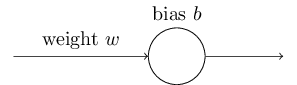
\includegraphics[width=0.9\textwidth]{images/tikz28.png}
\end{center}

\noindent 我们将训练这个神经元做一件简单得可笑的事：把输入 $1$ 变成输出 $0$. 当然，这是一个如此微不足道的任务，我们不用学习算法就能轻易地手算出合适的权重和偏置. 然而，用梯度下降来尝试学习权重和偏置却很有启发性. 所以让我们来看看这个神经元是如何学习的.

为了明确起见，我把初始权重设为 $0.6$，初始偏置设为 $0.9$. 这些是作为学习起点的通用选择，我并没有特意挑选它们. 神经元的初始输出是 $0.82$，所以在我们的神经元接近期望输出 $0.0$ 之前，需要进行相当多的学习. 点击下面右下角的 ``Run'' 来看看神经元如何学习到一个更接近 $0.0$ 的输出. 注意这不是预先录制的动画，你的浏览器实际上在计算梯度，然后用梯度更新权重和偏置，并显示结果. 学习率是 $\eta = 0.15$，事实证明这足够慢，让我们能跟上发生了什么，但又足够快，让我们在几秒钟内就能取得实质性的学习. 代价函数是第 1 章介绍的二次代价函数 $C$. 我很快就会提醒你代价函数的确切形式，所以不必去翻找定义. 注意你可以再次点击 ``Run'' 来多次运行动画.

如你所见，神经元迅速学到了一个权重和偏置，使代价下降，并使神经元的输出约为 $0.09$. 这并不完全是期望的输出 $0.0$，但已经相当不错了. 然而，假设我们改为把起始权重和起始偏置都设为 $2.0$. 在这种情况下，初始输出是 $0.98$，错得非常离谱. 让我们看看在这种情况下神经元如何学习输出 $0$. 再次点击 ``Run''：尽管这个例子使用了相同的学习率 ($\eta = 0.15$)，我们可以看到学习开始得慢得多. 事实上，在前 150 个左右的轮次中，权重和偏置几乎完全没有变化. 然后学习才开始起作用，并且和我们的第一个例子很像，神经元的输出迅速向 $0.0$ 靠近.

与人类学习相比，这种行为很奇怪. 正如我在本节开头所说，当我们对某件事错得很离谱时，我们往往学得最快. 但我们刚刚看到，我们的人工神经元在错得很离谱时学习有很大困难——比只是稍微错一点时困难得多. 更重要的是，事实证明这种行为不仅出现在这个玩具模型中，也出现在更一般的网络中. 为什么学习如此缓慢？我们能否找到一种避免这种减速的方法？

要理解这个问题的根源，请考虑我们的神经元是通过以由代价函数的偏导数 $\partial C/\partial w$ 和 $\partial C / \partial b$ 决定的速率改变权重和偏置来学习的. 所以，说 ``学习缓慢'' 实际上就等于说那些偏导数很小. 挑战在于理解它们为什么很小. 为了理解这一点，让我们计算这些偏导数. 回想一下，我们使用的是二次代价函数，根据方程 (6)

\begin{align*}
C(w,b) \equiv \frac{1}{2n} \sum_x \| y(x) - a\|^2 \nonumber
\end{align*}

\noindent，它由下式给出

\begin{equation}
C = \frac{(y-a)^2}{2},
\tag{54}
\end{equation}

\noindent 其中 $a$ 是使用训练输入 $x = 1$ 时神经元的输出，而 $y = 0$ 是对应的期望输出. 为了用权重和偏置更明确地写出这一点，回想一下 $a = \sigma(z)$，其中 $z = wx+b$. 使用链式法则对权重和偏置求导，我们得到

\begin{align}
\frac{\partial C}{\partial w} &= (a-y)\sigma'(z) x = a \sigma'(z) \tag{55} \\ \frac{\partial C}{\partial b} &= (a-y)\sigma'(z) = a \sigma'(z), \tag{56}
\end{align}

\noindent 其中我已代入 $x = 1$ 和 $y = 0$. 为了理解这些表达式的行为，让我们更仔细地看看右边的 $\sigma'(z)$ 项. 回想一下 $\sigma$ 函数的形状：我们可以从这个图中看到，当神经元的输出接近 $1$ 时，曲线变得非常平坦，因此 $\sigma'(z)$ 变得非常小. 方程 (55)

\begin{align*}
\frac{\partial C}{\partial w} &= (a-y)\sigma'(z) x = a \sigma'(z) \nonumber
\end{align*}

\noindent 和 (56)

\begin{align*}
\frac{\partial C}{\partial b} &= (a-y)\sigma'(z) = a \sigma'(z) \nonumber
\end{align*}

\noindent 然后告诉我们 $\partial C / \partial w$ 和 $\partial C / \partial b$ 变得非常小. 这就是学习缓慢的根源. 更重要的是，正如我们稍后将看到的，在更一般的神经网络中，学习缓慢的发生原因本质上相同，而不仅仅是我们一直在玩的这个玩具例子.
\subsectionTitle{交叉熵代价函数入门}{交叉熵代价函数入门}

我们如何解决学习缓慢的问题？事实证明，我们可以通过将二次代价替换为另一种称为交叉熵的代价函数来解决这个问题. 为了理解交叉熵，让我们稍微离开那个超级简单的玩具模型. 我们改为假设我们试图训练一个具有多个输入变量的神经元，$x_1, x_2, \ldots$，对应的权重 $w_1, w_2, \ldots$，以及一个偏置 $b$：

\begin{center}
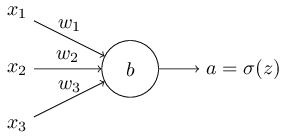
\includegraphics[width=0.9\textwidth]{images/tikz29.png}
\end{center}

\noindent 神经元的输出当然是 $a = \sigma(z)$，其中 $z = \sum_j w_j x_j+b$ 是输入的加权和. 我们为这个神经元定义交叉熵代价函数为

\begin{equation}
C = -\frac{1}{n} \sum_x \left[y \ln a + (1-y ) \ln (1-a) \right],
\tag{57}
\end{equation}

\noindent 其中 $n$ 是训练数据项的总数，求和是对所有训练输入 $x$ 进行的，而 $y$ 是对应的期望输出.

表达式 (57)

\begin{align*}
C = -\frac{1}{n} \sum_x \left[y \ln a + (1-y ) \ln (1-a) \right] \nonumber
\end{align*}

\noindent 能解决学习缓慢问题这一点并不明显. 事实上，坦率地说，把它称为代价函数是否合理甚至都不明显！在解决学习缓慢问题之前，让我们看看交叉熵在什么意义上可以被解释为代价函数.

有两个性质特别使得将交叉熵解释为代价函数是合理的. 首先，它是非负的，即 $C > 0$. 要看到这一点，请注意：(a) (57) 中求和里的所有各项

\begin{align*}
C = -\frac{1}{n} \sum_x \left[y \ln a + (1-y ) \ln (1-a) \right] \nonumber
\end{align*}

\noindent 都是负的，因为两个对数都是 $0$ 到 $1$ 范围内的数；并且 (b) 求和前面有一个负号.

其次，如果神经元对所有训练输入 $x$ 的实际输出都接近期望输出，那么交叉熵将接近零*\footnote{为了证明这一点，我需要假设期望输出 $y$ 都是 $0$ 或 $1$. 在解决分类问题时，例如，或者在计算布尔函数时，通常就是这种情况. 要理解当我们不做这个假设时会发生什么，请参见本节末尾的练习.}. 要看到这一点，例如假设对于某个输入 $x$，$y = 0$ 且 $a \approx 0$. 这是神经元在该输入上表现良好的情况. 我们看到代价表达式 (57)

\begin{align*}
C = -\frac{1}{n} \sum_x \left[y \ln a + (1-y ) \ln (1-a) \right] \nonumber
\end{align*}

\noindent 中的第一项消失了，因为 $y = 0$，而第二项就是 $-\ln (1-a) \approx 0$. 当 $y = 1$ 且 $a \approx 1$ 时也有类似的分析. 因此，只要实际输出接近期望输出，对代价的贡献就会很低.

总结起来，交叉熵是正的，并且当神经元对所有训练输入 $x$ 计算期望输出 $y$ 的能力越来越好时，它趋向于零. 这两个性质都是我们直觉上期望代价函数具有的. 事实上，二次代价也满足这两个性质. 所以这对交叉熵来说是个好消息. 但交叉熵代价函数的优点在于，与二次代价不同，它避免了学习减慢的问题. 要看到这一点，让我们计算交叉熵代价关于权重的偏导数. 我们将 $a = \sigma(z)$ 代入 (57)

\begin{align*}
C = -\frac{1}{n} \sum_x \left[y \ln a + (1-y ) \ln (1-a) \right] \nonumber
\end{align*}

\noindent，并应用两次链式法则，得到：

\begin{align}
\frac{\partial C}{\partial w_j} &= -\frac{1}{n} \sum_x \left( \frac{y }{\sigma(z)} -\frac{(1-y)}{1-\sigma(z)} \right) \frac{\partial \sigma}{\partial w_j} \tag{58} \\ &= -\frac{1}{n} \sum_x \left( \frac{y}{\sigma(z)} -\frac{(1-y)}{1-\sigma(z)} \right)\sigma'(z) x_j. \tag{59}
\end{align}

\noindent 将所有项放在公分母上并化简后，这变为：

\begin{equation}
\frac{\partial C}{\partial w_j} = \frac{1}{n} \sum_x \frac{\sigma'(z) x_j}{\sigma(z) (1-\sigma(z))} (\sigma(z)-y).
\tag{60}
\end{equation}

\noindent 利用 S 型函数的定义 $\sigma(z) = 1/(1+e^{-z})$，以及一点代数运算，我们可以证明 $\sigma'(z) = \sigma(z)(1-\sigma(z))$. 我会在下面的练习中请你验证这一点，但现在让我们暂且接受它. 我们看到 $\sigma'(z)$ 和 $\sigma(z)(1-\sigma(z))$ 项在上面的方程中相互抵消了，它简化为：

\begin{equation}
\frac{\partial C}{\partial w_j} = \frac{1}{n} \sum_x x_j(\sigma(z)-y).
\tag{61}
\end{equation}

\noindent 这是一个漂亮的表达式. 它告诉我们权重学习的速度由 $\sigma(z)-y$ 控制，即由输出中的误差控制. 误差越大，神经元学习得越快. 这正是我们直觉上期望的. 特别地，它避免了由二次代价的类似方程，即方程 (55)

\begin{align*}
\frac{\partial C}{\partial w} &= (a-y)\sigma'(z) x = a \sigma'(z) \nonumber
\end{align*}

\noindent 中的 $\sigma'(z)$ 项所导致的学习减慢. 当我们使用交叉熵时，$\sigma'(z)$ 项被抵消了，我们不再需要担心它很小. 这种抵消是交叉熵代价函数所保证的特殊奇迹. 实际上，这并不真的是一个奇迹. 正如我们稍后将看到的，交叉熵被特别选择正是为了具有这个性质.

以类似的方式，我们可以计算偏置的偏导数. 我不会再详细讲述所有细节，但你可以很容易地验证

\begin{equation}
\frac{\partial C}{\partial b} = \frac{1}{n} \sum_x (\sigma(z)-y).
\tag{62}
\end{equation}

\noindent 同样，这避免了由二次代价的类似方程，即方程 (56)

\begin{align*}
\frac{\partial C}{\partial b} &= (a-y)\sigma'(z) = a \sigma'(z) \nonumber
\end{align*}

\noindent 中的 $\sigma'(z)$ 项所导致的学习减慢.

\begin{exerciseBox}{练习}

\begin{itemize}

\item 验证 $\sigma'(z) = \sigma(z)(1-\sigma(z))$.

\end{itemize}

让我们回到之前玩过的玩具例子，探索当我们使用交叉熵而不是二次代价时会发生什么. 为了重新定位自己，我们将从二次代价表现良好的情况开始，起始权重为 $0.6$，起始偏置为 $0.9$. 按下 ``Run'' 看看当我们用交叉熵替换二次代价时会发生什么：不出所料，神经元在这个例子中学习得非常好，就像之前一样. 现在让我们看看我们的神经元之前卡住的情况（链接，用于比较），权重和偏置都从 $2.0$ 开始：成功了！这一次神经元学习得很快，正如我们所希望的那样. 如果你仔细观察，你可以看到代价曲线的斜率最初比二次代价对应曲线上初始平坦区域要陡峭得多. 正是这种陡峭性，交叉熵为我们带来的，防止我们在期望神经元学习最快的时候卡住，即当神经元一开始就错得离谱的时候.

我没有说明刚才展示的例子中使用了什么学习率. 之前，使用二次代价时，我们使用了 $\eta = 0.15$. 我们在新例子中应该使用相同的学习率吗？事实上，随着代价函数的改变，不可能精确地说使用 ``相同'' 学习率意味着什么；这是苹果和橘子的比较. 对于两种代价函数，我都只是通过实验来找到一个能够看清发生了什么事情的学习率. 如果你仍然好奇，尽管我否认了，这里是内幕：在刚才给出的例子中我使用了 $\eta = 0.005$.

你可能会反对说，学习率的变化使得上面的图变得毫无意义. 当我们的学习率选择一开始就是任意的时候，谁在乎神经元学习得有多快呢？！这种反对没有抓住要点. 这些图的要点不在于学习的绝对速度. 而在于学习速度如何变化. 特别地，当我们使用二次代价时，当神经元明显错误时学习比之后当神经元更接近正确输出时\emph{更慢}；而使用交叉熵时，当神经元明显错误时学习更快. 这些陈述不依赖于学习率是如何设置的.

我们一直在研究单个神经元的交叉熵. 然而，很容易将交叉熵推广到多神经元多层网络. 特别地，假设 $y = y_1, y_2, \ldots$ 是输出神经元，即最终层神经元的期望值，而 $a^L_1, a^L_2, \ldots$ 是实际输出值. 那么我们定义交叉熵为

\begin{equation}
C = -\frac{1}{n} \sum_x \sum_j \left[y_j \ln a^L_j + (1-y_j) \ln (1-a^L_j) \right].
\tag{63}
\end{equation}

\noindent 这与我们之前的表达式，即方程 (57)

\begin{align*}
C = -\frac{1}{n} \sum_x \left[y \ln a + (1-y ) \ln (1-a) \right] \nonumber
\end{align*}

\noindent 相同，只是现在我们用 $\sum_j$ 对所有输出神经元求和. 我不会明确地推导，但使用表达式 (63)

\begin{align*}
C = -\frac{1}{n} \sum_x \sum_j \left[y_j \ln a^L_j + (1-y_j) \ln (1-a^L_j) \right] \nonumber
\end{align*}

\noindent 在多神经元网络中避免学习减慢应该是合理的. 如果你感兴趣，你可以在下面的习题中进行推导.

顺便说一句，我使用 ``交叉熵'' 这个术语的方式让一些早期读者感到困惑，因为它表面上似乎与其他来源冲突. 特别地，通常将两个概率分布 $p_j$ 和 $q_j$ 的交叉熵定义为 $\sum_j p_j \ln q_j$. 这个定义可能与 (57)

\begin{align*}
C = -\frac{1}{n} \sum_x \left[y \ln a + (1-y ) \ln (1-a) \right] \nonumber
\end{align*}

\noindent 相关，如果我们把单个 S 型神经元视为输出一个由神经元的激活值 $a$ 及其补 $1-a$ 组成的概率分布.

然而，当我们在最终层有许多 S 型神经元时，激活值的向量 $a^L_j$ 通常不构成概率分布. 因此，像 $\sum_j p_j \ln q_j$ 这样的定义甚至没有意义，因为我们不是在处理概率分布. 相反，你可以把 (63)

\begin{align*}
C = -\frac{1}{n} \sum_x \sum_j \left[y_j \ln a^L_j + (1-y_j) \ln (1-a^L_j) \right] \nonumber
\end{align*}

\noindent 看作是一组逐神经元交叉熵的总和，每个神经元的激活值被解释为二元概率分布的一部分*\footnote{当然，在我们的网络中没有概率元素，所以它们不是真正的概率.}. 在这个意义上，(63)

\begin{align*}
C = -\frac{1}{n} \sum_x \sum_j \left[y_j \ln a^L_j + (1-y_j) \ln (1-a^L_j) \right] \nonumber
\end{align*}

\noindent 是概率分布交叉熵的推广.

我们什么时候应该使用交叉熵而不是二次代价？事实上，只要输出神经元是 S 型神经元，交叉熵几乎总是更好的选择. 要理解为什么，考虑当我们建立网络时，我们通常使用某种随机化来初始化权重和偏置. 可能发生的情况是，那些初始选择导致网络对某些训练输入决定性地错误——也就是说，一个输出神经元将在应该为 $0$ 时饱和在 $1$ 附近，或者反之. 如果我们使用二次代价，那将减慢学习. 它不会完全停止学习，因为权重将继续从其他训练输入中学习，但这显然是不可取的.

\end{exerciseBox}
\begin{exerciseBox}{练习}

\begin{itemize}

\item 交叉熵的一个容易出错之处在于，一开始很难记住 $y$ 和 $a$ 各自扮演的角色. 人们很容易搞混正确的形式究竟是 $-[y \ln a + (1-y) \ln (1-a)]$ 还是 $-[a \ln y + (1-a) \ln (1-y)]$. 当 $y = 0$ 或 $1$ 时，第二个表达式会发生什么？第一个表达式是否也有这个问题？为什么有或为什么没有？

\item
在本节开头的单神经元讨论中，我论证了如果对所有训练输入都有 $\sigma(z) \approx y$，那么交叉熵就很小. 该论证依赖于 $y$ 等于 $0$ 或 $1$. 这在分类问题中通常是成立的，但对于其他问题（例如回归问题），$y$ 有时可能取介于 $0$ 和 $1$ 之间的值. 证明当对所有训练输入都有 $\sigma(z) = y$ 时，交叉熵仍然取最小值. 在这种情况下，交叉熵的值为：

\begin{equation}
C = -\frac{1}{n} \sum_x [y \ln y+(1-y) \ln(1-y)].
\tag{64}
\end{equation}

量 $-[y \ln y+(1-y)\ln(1-y)]$ 有时被称为二元熵.

\end{itemize}

\end{exerciseBox}

\begin{exerciseBox}{习题}

\begin{itemize}

\item
\textbf{多层多神经元网络} 用上一章引入的记号，证明对于二次代价，关于输出层权重的偏导数为

\begin{equation}
\frac{\partial C}{\partial w^L_{jk}} = \frac{1}{n} \sum_x a^{L-1}_k (a^L_j-y_j) \sigma'(z^L_j).
\tag{65}
\end{equation}

项 $\sigma'(z^L_j)$ 会在输出神经元在错误的值上饱和时导致学习变慢. 证明对于交叉熵代价，单个训练样本 $x$ 的输出误差 $\delta^L$ 为

\begin{equation}
\delta^L = a^L-y.
\tag{66}
\end{equation}

利用这个表达式证明关于输出层权重的偏导数为

\begin{equation}
\frac{\partial C}{\partial w^L_{jk}} = \frac{1}{n} \sum_x a^{L-1}_k (a^L_j-y_j).
\tag{67}
\end{equation}

$\sigma'(z^L_j)$ 项消失了，因此交叉熵避免了学习变慢的问题，不仅像我们之前看到的那样在用于单个神经元时如此，而且在多层多神经元网络中也是如此. 对这一分析稍作变化也适用于偏置. 如果这对你来说不明显，那么你也应该把那个分析推导一遍.

\item
\textbf{当输出层是线性神经元时使用二次代价} 假设我们有一个多层多神经元网络. 假设最后一层中的所有神经元都是 \emph{线性神经元}，这意味着没有应用 S 型激活函数，输出就是 $a^L_j = z^L_j$. 证明如果我们使用二次代价函数，那么单个训练样本 $x$ 的输出误差 $\delta^L$ 为

\begin{equation}
\delta^L = a^L-y.
\tag{68}
\end{equation}

与上一个习题类似，利用这个表达式证明关于输出层权重和偏置的偏导数为

\begin{align}
\frac{\partial C}{\partial w^L_{jk}} &= \frac{1}{n} \sum_x a^{L-1}_k (a^L_j-y_j) \tag{69} \\ \frac{\partial C}{\partial b^L_{j}} &= \frac{1}{n} \sum_x (a^L_j-y_j). \tag{70}
\end{align}

这表明如果输出神经元是线性神经元，那么二次代价不会引起任何学习变慢的问题. 在这种情况下，二次代价实际上是一个合适使用的代价函数.

\end{itemize}

\end{exerciseBox}
\subsectionTitle{用交叉熵分类 MNIST 数字}{用交叉熵分类 MNIST 数字}

交叉熵很容易作为使用梯度下降和反向传播进行学习的程序的一部分来实现. 我们将在本章后面这样做，开发我们之前用于分类 MNIST 手写数字的程序 \texttt{network.py} 的改进版本. 新程序称为 \texttt{network2.py}，它不仅包含交叉熵，还包含本章中开发的若干其他技术*\footnote{代码可在 GitHub 上获取.}. 现在，让我们看看我们的新程序分类 MNIST 数字的效果如何. 与第 1 章的情况一样，我们将使用一个有 $30$ 个隐藏神经元的网络，并使用 $10$ 的小批量大小. 我们将学习率设为 $\eta = 0.5$*\footnote{在第 1 章中我们使用了二次代价和学习率 $\eta = 3.0$. 如上所述，当代价函数改变时，无法确切说明使用``相同''学习率意味着什么. 对于这两种代价函数，我都进行了实验，以在给定其他超参数选择的情况下找到能提供接近最优性能的学习率. \\ \\ 顺便说一句，对于将交叉熵的学习率与二次代价的学习率联系起来，有一个非常粗略的一般性经验法则. 正如我们之前看到的，二次代价的梯度项中多了一个 $\sigma' = \sigma(1-\sigma)$ 项. 假设我们对 $\sigma$ 的取值求平均，$\int_0^1 d\sigma \sigma(1-\sigma) = 1/6$. 我们看到（非常粗略地），在相同学习率下，二次代价的学习速度平均慢 $6$ 倍. 这表明一个合理的起点是将二次代价的学习率除以 $6$. 当然，这个论证远非严格，不应过于当真. 尽管如此，它有时可以是一个有用的起点.} 并训练 $30$ 个轮次. \texttt{network2.py} 的接口与 \texttt{network.py} 略有不同，但应该仍然清楚发生了什么. 顺便说一句，你可以通过在 Python shell 中使用诸如 \texttt{help(network2.Network.SGD)} 之类的命令来获取关于 \texttt{network2.py} 接口的文档.

\begin{lstlisting}
>>> import mnist_loader
>>> training_data, validation_data, test_data = \
... mnist_loader.load_data_wrapper()
>>> import network2
>>> net = network2.Network([784, 30, 10], cost=network2.CrossEntropyCost)
>>> net.large_weight_initializer()
>>> net.SGD(training_data, 30, 10, 0.5, evaluation_data=test_data,
... monitor_evaluation_accuracy=True)

\end{lstlisting}

顺便注意，\texttt{net.large\_\allowbreak{}weight\_\allowbreak{}initializer()} 命令用于以与第 1 章所述相同的方式初始化权重和偏置. 我们需要运行这个命令，因为在本章后面我们将改变网络中默认的权重初始化. 运行上述命令序列的结果是一个准确率为 $95.49$ 百分比的网络. 这与我们在第 1 章中使用二次代价得到的结果 $95.42$ 百分比非常接近.

让我们也看看使用 $100$ 个隐藏神经元、交叉熵，而其他参数保持不变的情况. 在这种情况下，我们获得了 $96.82$ 百分比的准确率. 这比第 1 章的结果有了实质性的改进，当时我们使用二次代价获得了 $96.59$ 百分比的分类准确率. 这看起来可能变化很小，但考虑到错误率已从 $3.41$ 百分比降至 $3.18$ 百分比. 也就是说，我们消除了大约十四分之一的原始错误. 这是相当可观的改进.

令人鼓舞的是，交叉熵代价给出的结果与二次代价相似或更好. 然而，这些结果并不能确凿地证明交叉熵是更好的选择. 原因是我只花了很少的精力来选择诸如学习率、小批量大小等超参数. 要使这种改进真正令人信服，我们需要对这些超参数进行彻底的优化. 尽管如此，这些结果是令人鼓舞的，并强化了我们早先的理论论证，即交叉熵比二次代价是更好的选择.

顺便说一句，这是我们在本章乃至本书其余大部分内容中将会看到的一种普遍模式的一部分. 我们将开发一项新技术，尝试它，然后得到``改进的''结果. 当然，看到这样的改进是很好的. 但对此类改进的解释总是有问题的. 只有当我们付出巨大努力优化所有其他超参数后看到改进，它们才真正令人信服. 那是大量的工作，需要大量的计算能力，而我们通常不会进行如此详尽的调查. 相反，我们将基于像上面所做的那样的非正式测试继续进行. 尽管如此，你应该记住，此类测试达不到确凿的证明，并保持警惕，留意论证正在失效的迹象.

到目前为止，我们已经详细讨论了交叉熵. 既然它只给我们的 MNIST 结果带来很小的改进，为什么要付出这么多努力呢？在本章后面，我们将看到其他技术——特别是正则化——能带来更大的改进. 那么为什么如此关注交叉熵呢？部分原因是交叉熵是一种广泛使用的代价函数，因此值得好好理解. 但更重要的原因是，神经元饱和是神经网络中的一个重要问题，我们将在本书中反复回到这个问题. 因此，我详细讨论了交叉熵，因为它是一个很好的实验室，可以用来开始理解神经元饱和以及如何解决它.
\subsectionTitle{交叉熵是什么意思？从何而来？}{交叉熵是什么意思？从何而来？}

我们对交叉熵的讨论集中在代数分析和实际实现上. 这很有用，但它留下了一些更广泛的概念性问题没有回答，比如：交叉熵是什么意思？有没有某种直观的方式来思考交叉熵？以及我们最初是如何想到交叉熵的？

让我们从最后一个问题开始：最初是什么促使我们想到交叉熵的？假设我们已经发现了前面描述的学习缓慢现象，并且理解了其根源是方程 (55)

\begin{align*}
\frac{\partial C}{\partial w} &= (a-y)\sigma'(z) x = a \sigma'(z) \nonumber
\end{align*}

\noindent 和 (56)

\begin{align*}
\frac{\partial C}{\partial b} &= (a-y)\sigma'(z) = a \sigma'(z) \nonumber
\end{align*}

\noindent 中的 $\sigma'(z)$ 项. 盯着这些方程看一会儿之后，我们可能会想，是否有可能选择一个代价函数，使得 $\sigma'(z)$ 项消失. 在这种情况下，单个训练样本 $x$ 的代价 $C = C_x$ 将满足

\begin{align}
\frac{\partial C}{\partial w_j} &= x_j(a-y) \tag{71} \\ \frac{\partial C}{\partial b } &= (a-y). \tag{72}
\end{align}

\noindent 如果我们能选择代价函数使这些方程成立，那么它们将以一种简单的方式捕捉到这样一个直觉：初始误差越大，神经元学习得越快. 它们还将消除学习缓慢的问题. 事实上，从这些方程出发，我们现在将展示，仅仅通过跟随我们的数学直觉，就有可能推导出交叉熵的形式. 为了看到这一点，注意由链式法则我们有

\begin{equation}
\frac{\partial C}{\partial b} = \frac{\partial C}{\partial a} \sigma'(z).
\tag{73}
\end{equation}

\noindent 利用 $\sigma'(z) = \sigma(z)(1-\sigma(z)) = a(1-a)$，最后一个方程变为

\begin{equation}
\frac{\partial C}{\partial b} = \frac{\partial C}{\partial a} a(1-a).
\tag{74}
\end{equation}

\noindent 与方程 (72)

\begin{align*}
\frac{\partial C}{\partial b } &= (a-y) \nonumber
\end{align*}

\noindent 比较，我们得到

\begin{equation}
\frac{\partial C}{\partial a} = \frac{a-y}{a(1-a)}.
\tag{75}
\end{equation}

\noindent 对这个表达式关于 $a$ 积分得到

\begin{equation}
C = -[y \ln a + (1-y) \ln (1-a)]+ {\rm constant},
\tag{76}
\end{equation}

\noindent 其中包含一个积分常数. 这是单个训练样本 $x$ 对代价的贡献. 要得到完整的代价函数，我们必须对训练样本取平均，得到

\begin{equation}
C = -\frac{1}{n} \sum_x [y \ln a +(1-y) \ln(1-a)] + {\rm constant},
\tag{77}
\end{equation}

\noindent 这里的常数是每个训练样本各自常数的平均值. 于是我们看到，方程 (71)

\begin{align*}
\frac{\partial C}{\partial w_j} &= x_j(a-y) \nonumber
\end{align*}

\noindent 和 (72)

\begin{align*}
\frac{\partial C}{\partial b } &= (a-y) \nonumber
\end{align*}

\noindent 唯一地确定了交叉熵的形式，至多相差一个整体常数项. 交叉熵并不是什么奇迹般从虚空中拽出来的东西. 相反，它是我们可以通过一种简单而自然的方式发现的东西.

那么交叉熵的直观含义呢？我们应该如何理解它？深入解释这一点会把我带到比我想去的更远的地方. 然而，值得一提的是，有一种来自信息论领域的标准方式来解释交叉熵. 粗略地说，这个想法是交叉熵是惊讶程度的一种度量. 特别地，我们的神经元试图计算函数 $x \rightarrow y = y(x)$. 但它实际计算的是函数 $x \rightarrow a = a(x)$. 假设我们把 $a$ 看作神经元对 $y$ 为 $1$ 的估计概率，而 $1-a$ 是对 $y$ 的正确值为 $0$ 的估计概率. 那么交叉熵衡量的是，当我们得知 $y$ 的真实值时，平均而言我们有多``惊讶''. 如果输出是我们所预期的，我们得到的惊讶程度就低；如果输出是出乎意料的，惊讶程度就高. 当然，我还没有确切说明``惊讶''是什么意思，所以这也许看起来像是空话. 但事实上，有一种精确的信息论方式来说明惊讶的含义. 不幸的是，我不知道网上有关于这个主题的好的、简短的、自包含的讨论. 但如果你想深入挖掘，维基百科上有一个简短的总结，可以让你走上正确的轨道. 而细节可以通过阅读 Cover 和 Thomas 关于信息论的书中第 5 章关于 Kraft 不等式的材料来补充.

\begin{exerciseBox}{习题}

\begin{itemize}

\item
我们已经详细讨论了在使用二次代价训练的网络中，输出神经元饱和时可能发生的学习缓慢现象. 另一个可能抑制学习的因素是方程 (61)

\begin{align*}
\frac{\partial C}{\partial w_j} = \frac{1}{n} \sum_x x_j(\sigma(z)-y) \nonumber
\end{align*}

中 $x_j$ 项的存在. 由于这一项，当输入 $x_j$ 接近零时，对应的权重 $w_j$ 将学习得很慢. 解释为什么不可能通过巧妙地选择代价函数来消除 $x_j$ 项.

\end{itemize}

\end{exerciseBox}
\subsectionTitle{Softmax}{Softmax}

在本章中，我们将主要使用交叉熵代价来解决学习缓慢的问题. 然而，我想简要地描述解决该问题的另一种方法，它基于所谓的 \emph{softmax} 神经元层. 在本章的剩余部分中，我们实际上不会使用 softmax 层，所以如果你非常着急，可以跳到下一节. 然而，softmax 仍然值得理解，部分原因是它本身很有趣，部分原因是我们在第 6 章讨论深度神经网络时会使用 softmax 层.

Softmax 的思想是为我们的神经网络定义一种新型的输出层. 它的开始方式与 S 型层相同，通过形成加权输入*\footnote{在描述 softmax 时，我们将频繁使用上一章引入的记号. 如果你需要回顾该章以刷新关于记号含义的记忆，不妨重读那一章.} $z^L_j = \sum_{k} w^L_{jk} a^{L-1}_k + b^L_j$. 然而，我们不应用 S 型函数来获得输出. 相反，在 softmax 层中，我们对 $z^L_j$ 应用所谓的 \emph{softmax 函数}. 根据这个函数，第 $j$ 个输出神经元的激活值 $a^L_j$ 是

\begin{equation}
a^L_j = \frac{e^{z^L_j}}{\sum_k e^{z^L_k}},
\tag{78}
\end{equation}

\noindent 其中分母是对所有输出神经元求和.

如果你不熟悉 softmax 函数，方程 (78)

\begin{align*}
a^L_j = \frac{e^{z^L_j}}{\sum_k e^{z^L_k}} \nonumber
\end{align*}

\noindent 可能看起来相当晦涩. 我们为什么想要使用这个函数当然并不明显. 而且这能帮助我们解决学习缓慢问题也不明显. 为了更好地理解方程 (78)

\begin{align*}
a^L_j = \frac{e^{z^L_j}}{\sum_k e^{z^L_k}} \nonumber
\end{align*}

\noindent，假设我们有一个具有四个输出神经元的网络，以及四个对应的加权输入，我们将其记为 $z^L_1, z^L_2, z^L_3$ 和 $z^L_4$. 下面显示的是可调节的滑块，展示了加权输入的可能值，以及相应输出激活值的图形. 开始探索的一个好地方是使用底部的滑块来增加 $z^L_4$：

\begin{table}[htbp]
\centering
\small
\begin{tabular}{cc}
\toprule

$z^L_1 = $ & $a^L_1 = $ \\

\midrule

$z^L_2$ = & $a^L_2 = $ \\

$z^L_3$ = & $a^L_3 = $ \\

$z^L_4$ = & $a^L_4 = $ \\

\bottomrule
\end{tabular}
\end{table}

当你增加 $z^L_4$ 时，你会看到相应的输出激活值 $a^L_4$ 增加，而其他输出激活值减少. 类似地，如果你减少 $z^L_4$，那么 $a^L_4$ 将减少，而所有其他输出激活值将增加. 事实上，如果你仔细观察，你会发现在这两种情况下，其他激活值的总变化恰好补偿了 $a^L_4$ 的变化. 原因是输出激活值保证总是加起来等于 $1$，我们可以使用方程 (78)

\begin{align*}
a^L_j = \frac{e^{z^L_j}}{\sum_k e^{z^L_k}} \nonumber
\end{align*}

\noindent 和一点代数来证明：

\begin{equation}
\sum_j a^L_j = \frac{\sum_j e^{z^L_j}}{\sum_k e^{z^L_k}} = 1.
\tag{79}
\end{equation}

\noindent 因此，如果 $a^L_4$ 增加，那么其他输出激活值必须减少相同的总量，以确保所有激活值的总和保持为 $1$. 当然，类似的说法对所有其他激活值也成立.

方程 (78)

\begin{align*}
a^L_j = \frac{e^{z^L_j}}{\sum_k e^{z^L_k}} \nonumber
\end{align*}

\noindent 还意味着输出激活值都是正的，因为指数函数是正的. 将此与上一段的观察结合起来，我们看到 softmax 层的输出是一组正数，它们的总和为 $1$. 换句话说，softmax 层的输出可以被视为一个概率分布.

Softmax 层输出一个概率分布这一事实相当令人愉快. 在许多问题中，能够将输出激活值 $a^L_j$ 解释为网络对正确输出是 $j$ 的概率估计是很方便的. 例如，在 MNIST 分类问题中，我们可以将 $a^L_j$ 解释为网络对正确数字分类是 $j$ 的估计概率.

相比之下，如果输出层是 S 型层，那么我们当然不能假设激活值形成一个概率分布. 我不会明确证明这一点，但 S 型层的激活值通常不会形成概率分布，这应该是合理的. 因此，使用 S 型输出层时，我们对输出激活值没有这样简单的解释.

\begin{exerciseBox}{练习}

\begin{itemize}

\item 构造一个例子，明确说明在具有 S 型输出层的网络中，输出激活值 $a^L_j$ 并不总是加起来等于 $1$.

\end{itemize}

我们开始对 softmax 函数以及 softmax 层的行为方式有所感觉. 回顾一下我们目前的位置：方程 (78)

\begin{align*}
a^L_j = \frac{e^{z^L_j}}{\sum_k e^{z^L_k}} \nonumber
\end{align*}

\noindent 中的指数确保所有输出激活值都是正的. 而方程 (78)

\begin{align*}
a^L_j = \frac{e^{z^L_j}}{\sum_k e^{z^L_k}} \nonumber
\end{align*}

\noindent 分母中的求和确保 softmax 输出加起来等于 $1$. 所以那个特定的形式不再显得那么神秘：相反，它是一种确保输出激活值形成概率分布的自然方式. 你可以把 softmax 看作一种重新缩放 $z^L_j$ 的方式，然后将它们挤压在一起形成一个概率分布.

\end{exerciseBox}

\begin{exerciseBox}{练习}

\begin{itemize}

\item \textbf{Softmax 的单调性} 证明如果 $j = k$，则 $\partial a^L_j / \partial z^L_k$ 为正，如果 $j \neq k$，则为负. 因此，增加 $z^L_j$ 保证会增加相应的输出激活值 $a^L_j$，并会减少所有其他输出激活值. 我们已经通过滑块经验性地看到了这一点，但这是一个严格的证明.

\item \textbf{Softmax 的非局部性} S 型层的一个好处是输出 $a^L_j$ 是相应加权输入的函数，$a^L_j = \sigma(z^L_j)$. 解释为什么 softmax 层不是这种情况：任何特定的输出激活值 $a^L_j$ 都依赖于\emph{所有}加权输入.

\end{itemize}

\end{exerciseBox}

\begin{exerciseBox}{习题}

\begin{itemize}

\item \textbf{反转 softmax 层} 假设我们有一个带有 softmax 输出层的神经网络，并且激活值 $a^L_j$ 是已知的. 证明相应的加权输入具有形式 $z^L_j = \ln a^L_j + C$，其中 $C$ 是某个与 $j$ 无关的常数.

\end{itemize}

\textbf{学习缓慢问题：} 我们现在已经对 softmax 神经元层有了相当多的了解. 但我们还没有看到 softmax 层如何让我们解决学习缓慢问题. 为了理解这一点，让我们定义\emph{对数似然}代价函数. 我们将使用 $x$ 表示网络的训练输入，$y$ 表示相应的期望输出. 那么这个训练输入相关的对数似然代价是

\begin{equation}
C \equiv -\ln a^L_y.
\tag{80}
\end{equation}

\noindent 因此，例如，如果我们使用 MNIST 图像进行训练，并输入一张 $7$ 的图像，那么对数似然代价是 $-\ln a^L_7$. 为了看出这符合直觉，考虑网络表现良好的情况，即它确信输入是 $7$. 在这种情况下，它将估计相应概率 $a^L_7$ 的值接近 $1$，因此代价 $-\ln a^L_7$ 将很小. 相比之下，当网络表现不那么好时，概率 $a^L_7$ 将较小，代价 $-\ln a^L_7$ 将较大. 所以对数似然代价的行为正如我们期望代价函数的行为一样.

那么学习缓慢问题呢？为了分析这一点，回想一下学习缓慢的关键是量 $\partial C / \partial w^L_{jk}$ 和 $\partial C / \partial b^L_j$ 的行为. 我不会明确地进行推导——我会在下面的习题中要求你去做——但通过一点代数你可以证明*\footnote{注意我在这里滥用记号，以稍微不同的方式使用 $y$. 在上一段中，我们使用 $y$ 表示网络的期望输出——例如，如果输入一张 $7$ 的图像，则输出 ``$7$''. 但在接下来的方程中，我使用 $y$ 表示对应于 $7$ 的输出激活值向量，即一个除了第 $7$ 个位置为 $1$ 外其余全为 $0$ 的向量.}

\begin{align}
\frac{\partial C}{\partial b^L_j} &= a^L_j-y_j \tag{81} \\ \frac{\partial C}{\partial w^L_{jk}} &= a^{L-1}_k (a^L_j-y_j) \tag{82}
\end{align}

\noindent 这些方程与我们之前分析交叉熵时得到的类似表达式相同. 例如，比较方程 (82)

\begin{align*}
\frac{\partial C}{\partial w^L_{jk}} &= a^{L-1}_k (a^L_j-y_j) \nonumber
\end{align*}

\noindent 与方程 (67)

\begin{align*}
\frac{\partial C}{\partial w^L_{jk}} &= \frac{1}{n} \sum_x a^{L-1}_k (a^L_j-y_j). \nonumber
\end{align*}

\noindent. 这是同一个方程，尽管在后者中我对训练实例进行了平均. 而且，正如之前的分析一样，这些表达式确保我们不会遇到学习缓慢. 事实上，将带有对数似然代价的 softmax 输出层视为与带有交叉熵代价的 S 型输出层非常相似是很有用的.

鉴于这种相似性，你应该使用 S 型输出层和交叉熵，还是 softmax 输出层和对数似然？事实上，在许多情况下两种方法都效果很好. 在本章的剩余部分，我们将使用 S 型输出层和交叉熵代价. 稍后，在第 6 章中，我们将有时使用 softmax 输出层和对数似然代价. 切换的原因是为了让我们后面的一些网络更类似于某些有影响力的学术论文中的网络. 作为一个更普遍的原则，当你想要将输出激活值解释为概率时，softmax 加对数似然是值得使用的. 这并不总是一个关注点，但在涉及不相交类别的分类问题（如 MNIST）中可能很有用.

\end{exerciseBox}

\begin{exerciseBox}{习题}

\begin{itemize}

\item
推导方程 (81)

\begin{align*}
\frac{\partial C}{\partial b^L_j} &= a^L_j-y_j \nonumber
\end{align*}

和 (82)

\begin{align*}
\frac{\partial C}{\partial w^L_{jk}} &= a^{L-1}_k (a^L_j-y_j) \nonumber
\end{align*}

.

\item
\textbf{``softmax'' 这个名字从何而来？} 假设我们改变 softmax 函数，使得输出激活值由下式给出

\begin{equation}
a^L_j = \frac{e^{c z^L_j}}{\sum_k e^{c z^L_k}},
\tag{83}
\end{equation}

其中 $c$ 是一个正常数. 注意 $c = 1$ 对应于标准的 softmax 函数. 但如果我们使用不同的 $c$ 值，我们会得到一个不同的函数，尽管如此，它在定性上与 softmax 相当相似. 特别地，证明输出激活值形成一个概率分布，就像通常的 softmax 一样. 假设我们让 $c$ 变得很大，即 $c \rightarrow \infty$. 输出激活值 $a^L_j$ 的极限值是什么？解决这个问题后，你应该清楚为什么我们将 $c = 1$ 函数视为最大值函数的 ``软化'' 版本. 这就是 ``softmax'' 一词的起源.

\item
\textbf{使用 softmax 和对数似然代价的反向传播} 在上一章中，我们推导了包含 S 型层的网络的反向传播算法. 为了将算法应用于具有 softmax 层的网络，我们需要找出最终层中误差 $\delta^L_j \equiv \partial C / \partial z^L_j$ 的表达式. 证明一个合适的表达式是：

\begin{equation}
\delta^L_j = a^L_j -y_j.
\tag{84}
\end{equation}

使用这个表达式，我们可以将反向传播算法应用于使用 softmax 输出层和对数似然代价的网络.

\end{itemize}

\end{exerciseBox}
\sectionTitle{过拟合与正则化}{过拟合与正则化}

诺贝尔奖得主、物理学家 Enrico Fermi 曾被问及对某个数学模型的看法，该模型是一些同事为解决一个重要的未解物理问题而提出的. 这个模型与实验符合得非常好，但 Fermi 持怀疑态度. 他问模型中可以设定多少个自由参数. 答案是``四个''.Fermi 回答说*\footnote{这句话出自 Freeman Dyson 的一篇妙趣横生的文章，Dyson 正是提出那个有缺陷模型的人之一. 一头四参数的大象可以在这里找到.}：``我记得我的朋友 Johnny von Neumann 曾说过，给我四个参数，我能拟合出一头大象，给我五个参数，我能让它甩鼻子.''.

当然，关键在于，拥有大量自由参数的模型可以描述范围惊人的广泛现象. 即使这样的模型与现有数据吻合得很好，也不能说明它就是一个好模型. 这可能只是意味着模型中有足够的自由度，使它几乎能描述任何给定规模的数据集，而并未捕捉到关于底层现象的真正洞见. 当这种情况发生时，模型对现有数据表现良好，但无法泛化到新情境. 对模型的真正检验，是它在之前未曾接触过的情境中做出预测的能力.

Fermi 和 von Neumann 对拥有四个参数的模型持怀疑态度. 我们用于分类 MNIST 数字的 30 个隐藏神经元网络有将近 24,000 个参数！这真是很多参数. 我们的 100 个隐藏神经元网络有将近 80,000 个参数，而最先进的深度神经网络有时包含数百万甚至数十亿个参数. 我们应该相信这些结果吗？

让我们通过构造一个网络在新情境中泛化表现不佳的场景，来把这个问题说得更清楚. 我们将使用 30 个隐藏神经元的网络，它有 23,860 个参数. 但我们不会用全部 50,000 张 MNIST 训练图像来训练网络. 相反，我们只使用前 1,000 张训练图像. 使用这个受限的集合将使泛化问题更加明显. 我们将采用与之前类似的方式进行训练，使用交叉熵代价函数，学习率为 $\eta = 0.5$，小批量大小为 $10$. 不过，我们将训练 400 个轮次，比之前稍多一些，因为我们没有使用那么多训练样本. 让我们用 \texttt{network2} 来观察代价函数的变化方式：

\begin{lstlisting}

>>> import mnist_loader
>>> training_data, validation_data, test_data = \
... mnist_loader.load_data_wrapper()
>>> import network2
>>> net = network2.Network([784, 30, 10], cost=network2.CrossEntropyCost)
>>> net.large_weight_initializer()
>>> net.SGD(training_data[:1000], 400, 10, 0.5, evaluation_data=test_data,
... monitor_evaluation_accuracy=True, monitor_training_cost=True)

\end{lstlisting}

利用这些结果，我们可以绘制出代价随网络学习而变化的方式*\footnote{这张图以及接下来的四张图都是由程序 overfitting.py 生成的.}：

\begin{center}
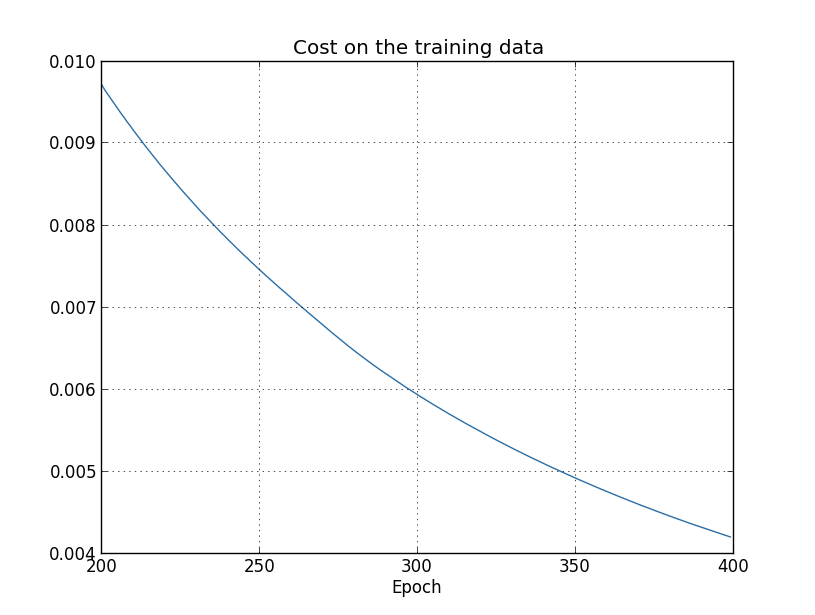
\includegraphics[width=0.867\textwidth]{images/overfitting1.png}
\end{center}

\noindent 这看起来令人鼓舞，显示出代价平滑下降，正如我们所预期的那样. 请注意，我只展示了第 200 到第 399 个训练轮次. 这让我们能够近距离地观察学习后期的阶段，而正如我们将看到的，有趣的事情恰恰发生在这里.

现在让我们看看测试数据上的分类准确率如何随时间变化：

\begin{center}
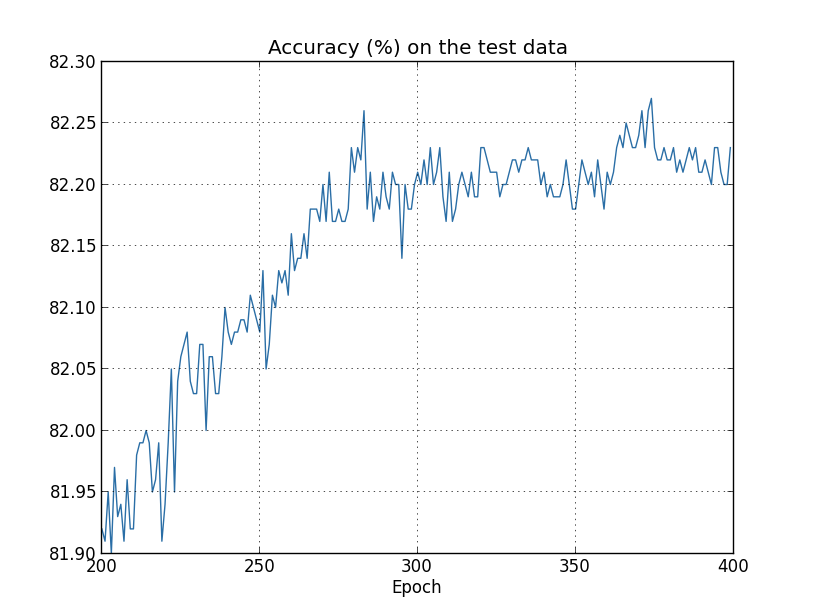
\includegraphics[width=0.867\textwidth]{images/overfitting2.png}
\end{center}

\noindent 同样，我做了相当程度的放大. 在前 200 个轮次（未显示）中，准确率上升到略低于 82\% 的水平. 然后学习逐渐放缓. 最后，在第 280 个轮次左右，分类准确率基本停止改善. 之后的轮次只是在第 280 个轮次的准确率值附近出现小的随机波动. 将此与之前的图对比，那里训练数据对应的代价仍在平滑下降. 如果我们只看那个代价，似乎我们的模型仍在变得``更好''. 但测试准确率的结果表明这种改善是一种错觉. 就像 Fermi 不喜欢的那个模型一样，我们的网络在第 280 个轮次之后学到的东西不再能泛化到测试数据. 因此这不是有用的学习. 我们说网络在第 280 个轮次之后发生了\emph{过拟合}或\emph{过度训练}.

你可能会想，这里的问题是不是我在看训练数据上的\emph{代价}，而不是测试数据上的\emph{分类准确率}. 换句话说，也许问题在于我们在做苹果和橘子的比较. 如果我们把训练数据上的代价与测试数据上的代价进行比较，也就是比较相似的度量，会怎样呢？或者我们可以比较训练数据和测试数据上的分类准确率？事实上，无论我们怎样比较，本质上都会出现同样的现象. 不过细节确实会有所不同. 例如，让我们看看测试数据上的代价：

\begin{center}
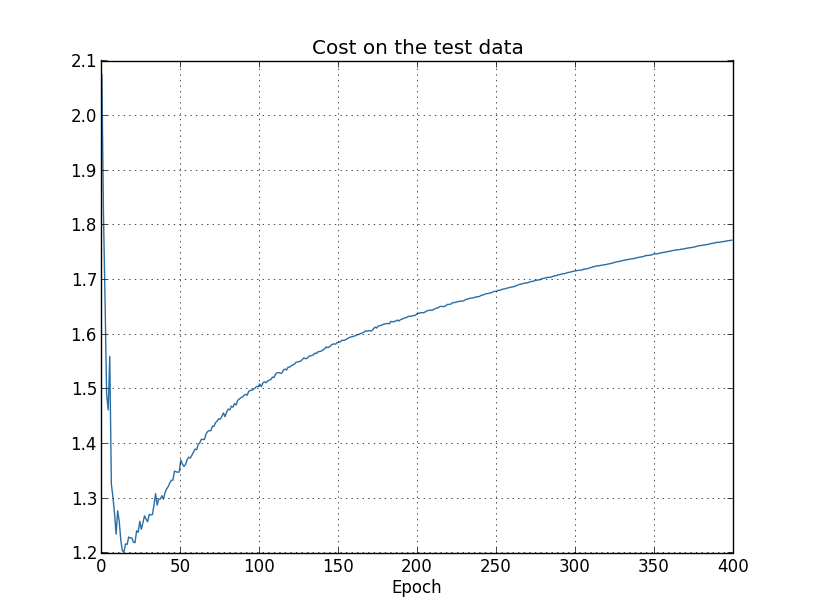
\includegraphics[width=0.867\textwidth]{images/overfitting3.png}
\end{center}

\noindent 我们可以看到，测试数据上的代价在第 15 个轮次左右之前一直在改善，但之后实际上开始变差，尽管训练数据上的代价仍在继续改善. 这是我们的模型正在过拟合\label{term:54}的另一个迹象. 不过，这提出了一个难题：我们应该把第 15 个轮次还是第 280 个轮次视为过拟合开始主导学习的节点？从实践的角度来看，我们真正关心的是提高测试数据上的分类准确率，而测试数据上的代价不过是分类准确率的一个代理指标. 因此，把第 280 个轮次视为我们的神经网络中过拟合开始主导学习的节点是最合理的.

过拟合的另一个迹象可以在训练数据上的分类准确率中看到：

\begin{center}
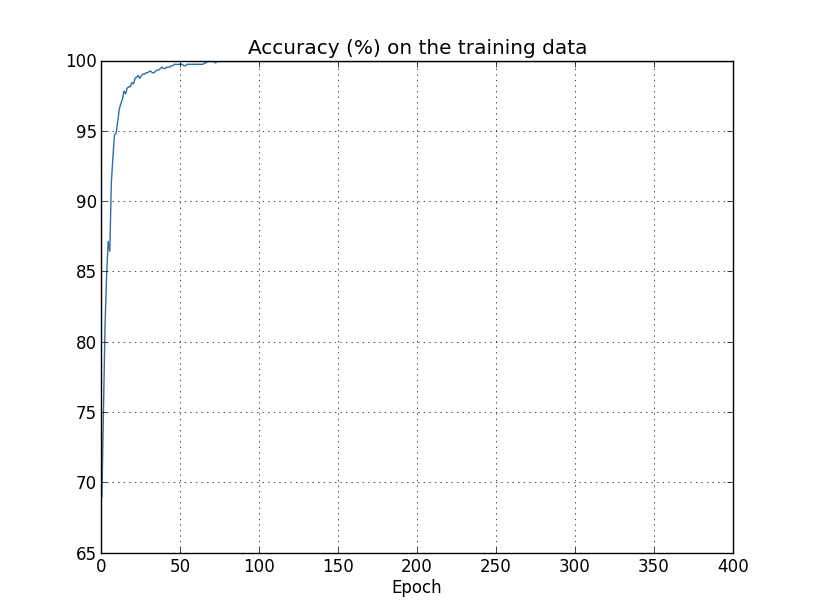
\includegraphics[width=0.867\textwidth]{images/overfitting4.png}
\end{center}

\noindent 准确率一路上升到 $100$\%. 也就是说，我们的网络正确地分类了全部 $1,000$ 张训练图像！与此同时，我们的测试准确率最高只有 $82.27$\% . 所以我们的网络确实是在学习训练集的特殊性，而不仅仅是在一般意义上识别数字. 几乎可以说，我们的网络只是在记忆训练集，而没有充分理解数字以便泛化到测试集\label{term:55}.

过拟合是神经网络中的一个主要问题. 在现代网络中尤其如此，因为这些网络通常拥有非常大量的权重和偏置. 为了有效地训练，我们需要一种检测过拟合何时发生的方法，这样我们就不会过度训练. 我们还希望有减少过拟合影响的技术.

检测过拟合的显而易见的方法是使用上面的做法，在网络训练过程中跟踪测试数据上的准确率. 如果我们看到测试数据上的准确率不再改善，就应该停止训练. 当然，严格来说，这并不一定是过拟合的迹象. 也可能是测试数据和训练数据上的准确率同时停止改善. 尽管如此，采用这一策略可以防止过拟合.

事实上，我们将使用这一策略的一个变体. 回想一下，当我们加载 MNIST 数据时，我们加载了三个数据集：

\begin{lstlisting}

>>> import mnist_loader
>>> training_data, validation_data, test_data = \
... mnist_loader.load_data_wrapper()

\end{lstlisting}

到目前为止，我们一直在使用 training\_\allowbreak{}data 和 test\_\allowbreak{}data，而忽略了 validation\_\allowbreak{}data.validation\_\allowbreak{}data 包含 $10,000$ 张数字图像，这些图像不同于 MNIST 训练集中的 $50,000$ 张图像，也不同于 MNIST 测试集中的 $10,000$ 张图像. 我们将使用 validation\_\allowbreak{}data 而不是 test\_\allowbreak{}data 来防止过拟合. 为此，我们将使用与上面针对 test\_\allowbreak{}data 所描述的几乎相同的策略. 也就是说，我们将在每个轮次结束时计算 validation\_\allowbreak{}data 上的分类准确率. 一旦 validation\_\allowbreak{}data 上的分类准确率饱和，我们就停止训练. 这一策略被称为提前停止\label{term:56}. 当然，在实践中我们不会立即知道准确率何时饱和. 相反，我们会继续训练，直到我们确信准确率已经饱和* *判断何时停止需要一些判断力. 在我之前的图中，我把第 280 个轮次确定为准确率饱和的位置. 这可能过于悲观了. 神经网络在训练中有时会停滞一段时间，然后继续改善. 如果更多的学习能在第 400 个轮次之后仍然发生，我也不会感到惊讶，尽管任何进一步改善的幅度可能很小. 因此，可以采用或多或少激进的提前停止策略..

为什么要使用 \texttt{validation\_\allowbreak{}data} 而不是 \texttt{test\_\allowbreak{}data} 来防止过拟合？事实上，这是一个更一般策略的一部分，即使用 \texttt{validation\_\allowbreak{}data} 来评估超参数的不同试验选择，例如训练的轮次数、学习率、最佳网络结构等等. 我们使用这样的评估来找到并设定超参数的良好值. 确实，尽管我直到现在才提到，但这在一定程度上就是我在本书前面做出超参数选择的方式.（稍后会详细讨论.）

当然，这丝毫没有回答为什么我们使用 \texttt{validation\_\allowbreak{}data} 而不是 \texttt{test\_\allowbreak{}data} 来防止过拟合的问题. 相反，它把这个问题替换成了一个更一般的问题：为什么我们使用 \texttt{validation\_\allowbreak{}data} 而不是 \texttt{test\_\allowbreak{}data} 来设定良好的超参数？要理解原因，请考虑在设定超参数时，我们很可能会尝试许多不同的超参数选择. 如果我们基于对 \texttt{test\_\allowbreak{}data} 的评估来设定超参数，就有可能最终把超参数过拟合到 \texttt{test\_\allowbreak{}data} 上. 也就是说，我们可能最终找到的超参数拟合了 \texttt{test\_\allowbreak{}data} 的特定特殊性，但网络的性能无法泛化到其他数据集. 我们通过使用 \texttt{validation\_\allowbreak{}data} 来确定超参数来防范这一点. 然后，一旦我们得到了想要的超参数，我们就使用 \texttt{test\_\allowbreak{}data} 做最终的准确率评估. 这让我们确信，我们在 \texttt{test\_\allowbreak{}data} 上的结果是我们的神经网络泛化能力的真实度量. 换一种说法，你可以把验证数据看作一种训练数据，它帮助我们学习良好的超参数. 这种寻找良好超参数的方法有时被称为\emph{留出}法，因为 \texttt{validation\_\allowbreak{}data} 被分离出来或``留出''于 \texttt{training\_\allowbreak{}data}.

现在，在实践中，即使在 \texttt{test\_\allowbreak{}data} 上评估了性能之后，我们也可能改变主意，想要尝试另一种方法——也许是不同的网络结构——这将涉及找到一组新的超参数. 如果我们这样做，难道不存在最终也会对 \texttt{test\_\allowbreak{}data} 过拟合的危险吗？我们是否需要潜在无限回归的数据集，才能确信我们的结果会泛化？完全解决这一顾虑是一个深刻而困难的问题. 但就我们的实际目的而言，我们不会过多担心这个问题. 相反，我们将继续前进，使用基本的留出法，基于 \texttt{training\_\allowbreak{}data}、\texttt{validation\_\allowbreak{}data} 和 \texttt{test\_\allowbreak{}data}，如上所述.

到目前为止，我们一直在看只使用 1,000 张训练图像时的过拟合. 当我们使用完整的 50,000 张图像训练集时会发生什么？我们将保持所有其他参数不变（30 个隐藏神经元、学习率 0.5、小批量大小 10），但使用全部 50,000 张图像训练 30 个轮次. 下面这张图展示了训练数据和测试数据上分类准确率的结果. 请注意，我在这里使用了测试数据而不是验证数据，以便使结果与之前的图更直接地可比.

\begin{center}
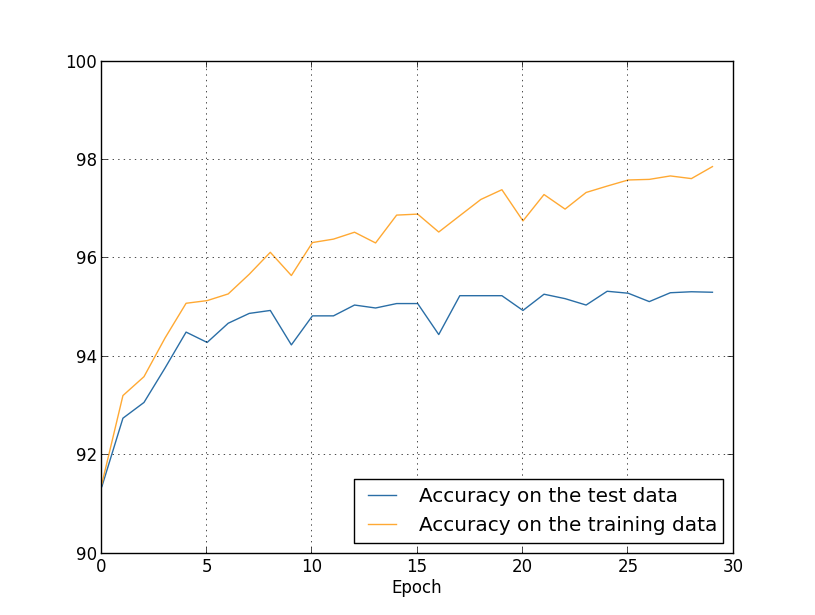
\includegraphics[width=0.867\textwidth]{images/overfitting_full.png}
\end{center}

如你所见，测试数据和训练数据上的准确率比我们使用 1,000 个训练样本时保持得更加接近. 特别是，训练数据上最好的分类准确率 $97.86$\% 仅比测试数据上的 $95.33$\% 高出 $2.53$\% . 这与我们之前 $17.73$\% 的差距相比！过拟合仍在发生，但已经大大减少了. 我们的网络从训练数据到测试数据的泛化能力好多了. 一般来说，减少过拟合的最佳方法之一就是增加训练数据的大小. 有了足够的训练数据，即使是非常大的网络也很难过拟合. 不幸的是，训练数据可能很昂贵或难以获取，所以这并不总是一个实际的选择.
\subsectionTitle{正则化}{正则化}

增加训练数据量是减少过拟合的一种方法. 我们还有其他方法可以减少过拟合的程度吗？一种可能的方法是缩小网络的规模. 然而，大型网络有可能比小型网络更强大，因此我们只会不情愿地采用这个选项.

幸运的是，还有其他技术可以减少过拟合，即使我们拥有固定的网络和固定的训练数据. 这些技术被称为\emph{正则化}技术. 在本节中，我将描述最常用的正则化技术之一，这种技术有时被称为\emph{权重衰减}或\emph{L2 正则化}. L2 正则化的思想是在代价函数中添加一个额外的项，这个项被称为\emph{正则化项}. 下面是正则化的交叉熵：

\begin{equation}
C = -\frac{1}{n} \sum_{xj} \left[ y_j \ln a^L_j+(1-y_j) \ln (1-a^L_j)\right] + \frac{\lambda}{2n} \sum_w w^2.
\tag{85}
\end{equation}

\noindent 第一项就是交叉熵的通常表达式. 但我们添加了第二项，即网络中所有\emph{权重}的平方和. 它被一个因子 $\lambda / 2n$ 缩放，其中 $\lambda > 0$ 被称为\emph{正则化参数}，而 $n$ 一如既往地是我们训练集的大小. 我稍后会讨论如何选择 $\lambda$. 同样值得注意的是，正则化项\emph{不}包含偏置. 我下面也会回到这一点.

当然，也可以对其他代价函数进行正则化，例如二次代价. 这可以用类似的方式完成：

\begin{equation}
C = \frac{1}{2n} \sum_x \|y-a^L\|^2 + \frac{\lambda}{2n} \sum_w w^2.
\tag{86}
\end{equation}

\noindent 在这两种情况下，我们可以将正则化的代价函数写为

\begin{equation}
C = C_0 + \frac{\lambda}{2n} \sum_w w^2,
\tag{87}
\end{equation}

\noindent 其中 $C_0$ 是原始的、未正则化的代价函数.

直观地说，正则化的效果是使网络在其他条件相同的情况下倾向于学习较小的权重. 只有当较大的权重能显著改善代价函数的第一部分时，它们才会被允许. 换句话说，正则化可以被视为在寻找小权重和最小化原始代价函数之间的一种折衷方式. 折衷中两个元素的相对重要性取决于 $\lambda$ 的值：当 $\lambda$ 很小时，我们倾向于最小化原始代价函数，但当 $\lambda$ 很大时，我们倾向于较小的权重.

现在，为什么做出这种折衷应该有助于减少过拟合，这一点其实一点也不明显！但事实证明它确实有帮助. 我们将在下一节中讨论它为什么有帮助的问题. 但首先，让我们通过一个例子来展示正则化确实能减少过拟合.

为了构造这样一个例子，我们首先需要弄清楚如何在正则化的神经网络中应用我们的随机梯度下降学习算法. 特别地，我们需要知道如何计算网络中所有权重和偏置的偏导数 $\partial C / \partial w$ 和 $\partial C / \partial b$. 对公式 (87) 求偏导数

\begin{align*}
C = C_0 + \frac{\lambda}{2n} \sum_w w^2 \nonumber
\end{align*}

\noindent 得到

\begin{align}
\frac{\partial C}{\partial w} &= \frac{\partial C_0}{\partial w} + \frac{\lambda}{n} w \tag{88} \\ \frac{\partial C}{\partial b} &= \frac{\partial C_0}{\partial b}. \tag{89}
\end{align}

\noindent $\partial C_0 / \partial w$ 和 $\partial C_0 / \partial b$ 项可以使用反向传播来计算，如上一章所述. 因此我们看到，计算正则化代价函数的梯度很容易：像往常一样使用反向传播，然后在所有\emph{权重}项的偏导数上加上 $\frac{\lambda}{n} w$. 关于偏置的偏导数保持不变，因此偏置的梯度下降学习规则与通常的规则相同：

\begin{equation}
b \rightarrow b -\eta \frac{\partial C_0}{\partial b}.
\tag{90}
\end{equation}

\noindent 权重的学习规则变为：

\begin{align}
w &\rightarrow w-\eta \frac{\partial C_0}{\partial w}-\frac{\eta \lambda}{n} w \tag{91} \\ &= \left(1-\frac{\eta \lambda}{n}\right) w -\eta \frac{\partial C_0}{\partial w}. \tag{92}
\end{align}

\noindent 这与通常的梯度下降学习规则完全相同，只是我们首先将权重 $w$ 乘以一个因子 $1-\frac{\eta \lambda}{n}$ 进行缩放. 这种缩放有时被称为\emph{权重衰减}，因为它使权重变小. 乍一看，这似乎意味着权重被不可阻挡地推向零. 但这是不对的，因为如果这样做能导致未正则化的代价函数减小，另一项可能会导致权重增加.

好了，这就是梯度下降的工作原理. 那随机梯度下降呢？嗯，就像在未正则化的随机梯度下降中一样，我们可以通过对 $m$ 个训练样本的小批量进行平均来估计 $\partial C_0 / \partial w$. 因此，随机梯度下降的正则化学习规则变为（参见公式 (20)

\begin{align*}
w_k &\rightarrow w_k' = w_k-\frac{\eta}{m} \sum_j \frac{\partial C_{X_j}}{\partial w_k} \nonumber
\end{align*}

\noindent ）

\begin{equation}
w \rightarrow \left(1-\frac{\eta \lambda}{n}\right) w -\frac{\eta}{m} \sum_x \frac{\partial C_x}{\partial w},
\tag{93}
\end{equation}

\noindent 其中求和是对小批量中的训练样本 $x$ 进行的，而 $C_x$ 是每个训练样本的（未正则化的）代价. 这与随机梯度下降的通常规则完全相同，除了 $1-\frac{\eta \lambda}{n}$ 权重衰减\label{term:57}因子. 最后，为了完整起见，让我陈述一下偏置的正则化学习规则. 当然，这与未正则化的情况完全相同（参见公式 (21)

\begin{align*}
b_l &\rightarrow b_l' = b_l-\frac{\eta}{m} \sum_j \frac{\partial C_{X_j}}{\partial b_l} \nonumber
\end{align*}

\noindent ），

\begin{equation}
b \rightarrow b - \frac{\eta}{m} \sum_x \frac{\partial C_x}{\partial b},
\tag{94}
\end{equation}

\noindent 其中求和是对小批量中的训练样本 $x$ 进行的.

让我们看看正则化如何改变我们神经网络的性能. 我们将使用一个有 $30$ 个隐藏神经元的网络，小批量大小为 $10$，学习率为 $0.5$，并使用交叉熵代价函数. 然而，这次我们将使用 $\lambda = 0.1$ 的正则化参数. 注意，在代码中，我们使用变量名 \texttt{lmbda}，因为 \texttt{lambda} 是 Python 中的保留字，含义与此无关. 我还再次使用了 \texttt{test\_\allowbreak{}data}，而不是 \texttt{validation\_\allowbreak{}data}. 严格来说，出于我们之前讨论过的所有原因，我们应该使用 \texttt{validation\_\allowbreak{}data}. 但我决定使用 \texttt{test\_\allowbreak{}data}，因为它使结果与我们之前未正则化的结果更直接可比. 你可以轻松地将代码改为使用 \texttt{validation\_\allowbreak{}data}，你会发现它给出了类似的结果.

\begin{lstlisting}

>>> import mnist_loader
>>> training_data, validation_data, test_data = \
... mnist_loader.load_data_wrapper()
>>> import network2
>>> net = network2.Network([784, 30, 10], cost=network2.CrossEntropyCost)
>>> net.large_weight_initializer()
>>> net.SGD(training_data[:1000], 400, 10, 0.5,
... evaluation_data=test_data, lmbda = 0.1,
... monitor_evaluation_cost=True, monitor_evaluation_accuracy=True,
... monitor_training_cost=True, monitor_training_accuracy=True)

\end{lstlisting}

训练数据上的代价在整个过程中都在下降，与之前未正则化的情况非常相似* *这个图和接下来两个图是用程序 overfitting.py 生成的.：

\begin{center}
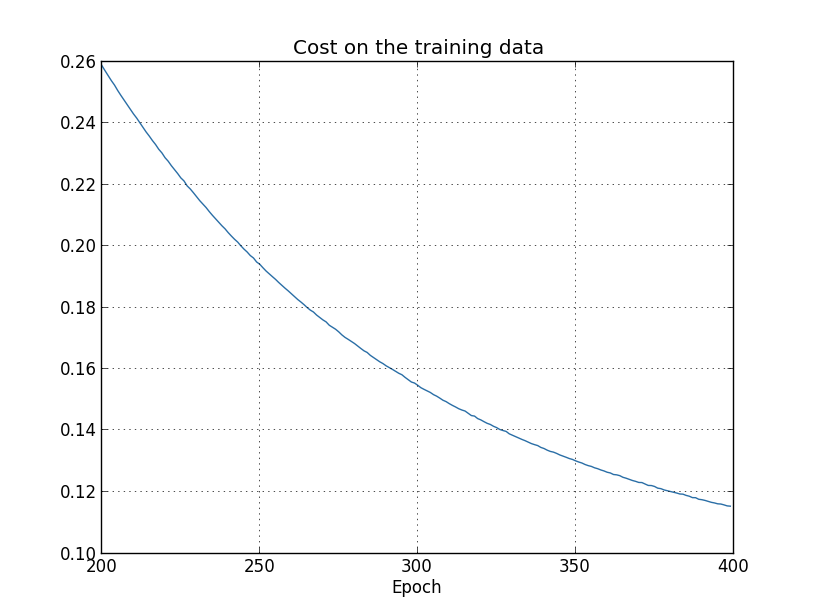
\includegraphics[width=0.867\textwidth]{images/regularized1.png}
\end{center}

\noindent 但这次 \texttt{test\_\allowbreak{}data} 上的准确率在整个 400 个轮次中持续增加：

\begin{center}
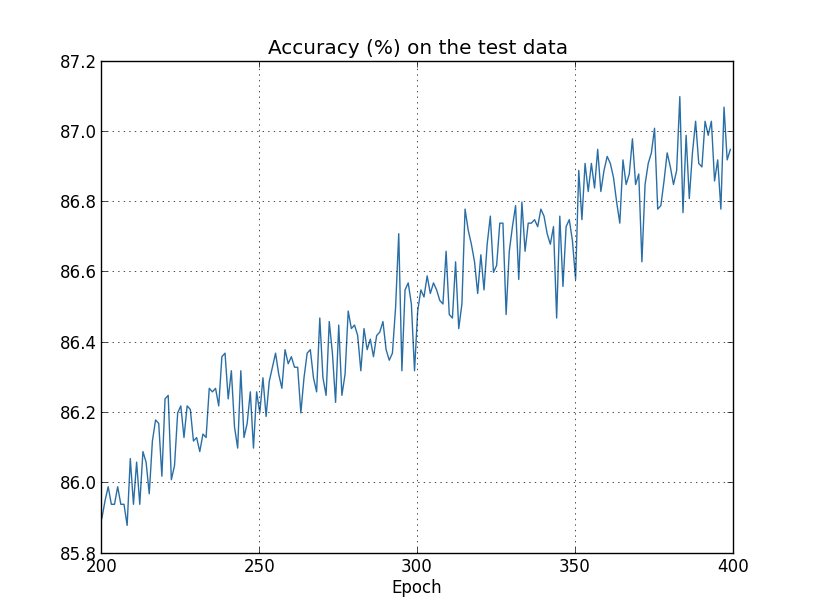
\includegraphics[width=0.867\textwidth]{images/regularized2.png}
\end{center}

\noindent 显然，正则化的使用抑制了过拟合. 更重要的是，准确率显著提高，峰值分类准确率为 $87.1$ 百分比，而未正则化情况下获得的峰值为 $82.27$ 百分比. 事实上，通过继续训练超过 400 个轮次，我们几乎肯定可以获得相当好的结果. 从经验上看，正则化似乎使我们的网络泛化得更好，并显著减少了过拟合的影响.

如果我们走出只有 1,000 张训练图像的人为环境，回到完整的 50,000 张图像训练集，会发生什么？当然，我们已经看到，在完整的 50,000 张图像下，过拟合问题要小得多. 正则化还有进一步的帮助吗？让我们保持超参数与之前相同——$30$ 个轮次，学习率 $0.5$，小批量大小为 $10$. 然而，我们需要修改正则化参数. 原因是训练集的大小 $n$ 从 $n = 1,000$ 变为 $n = 50,000$，这改变了权重衰减因子 $1 - \frac{\eta \lambda}{n}$. 如果我们继续使用 $\lambda = 0.1$，那将意味着权重衰减少得多，因此正则化效果也小得多. 我们通过改为 $\lambda = 5.0$ 来补偿.

好了，让我们训练我们的网络，首先停下来重新初始化权重：

\begin{lstlisting}

>>> net.large_weight_initializer()
>>> net.SGD(training_data, 30, 10, 0.5,
... evaluation_data=test_data, lmbda = 5.0,
... monitor_evaluation_accuracy=True, monitor_training_accuracy=True)

\end{lstlisting}

我们得到结果：

\begin{center}
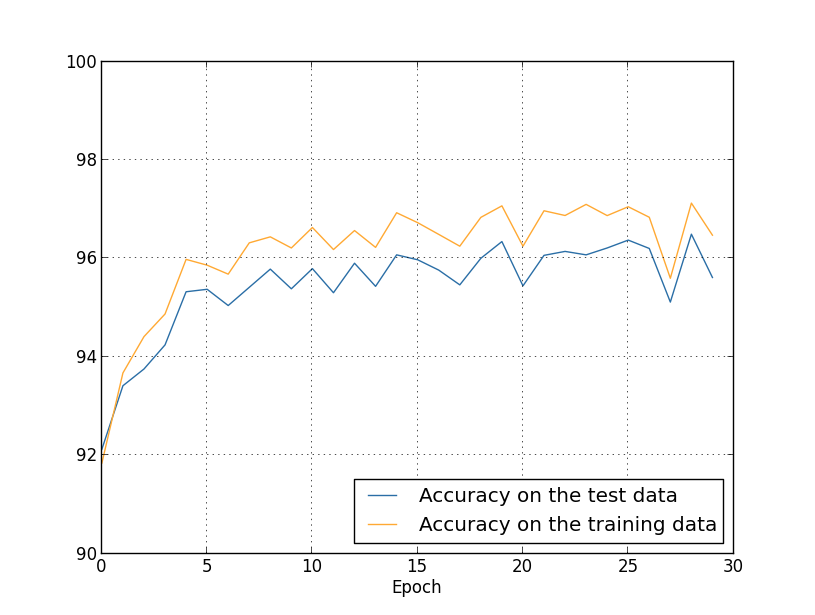
\includegraphics[width=0.867\textwidth]{images/regularized_full.png}
\end{center}

\noindent 这里有很多好消息. 首先，我们在测试数据上的分类准确率提高了，从未正则化时的 $95.49$ 百分比提高到 $96.49$ 百分比. 这是一个很大的改进. 其次，我们可以看到训练数据和测试数据上的结果之间的差距比以前小得多，不到一个百分点. 这仍然是一个显著的差距，但我们显然在减少过拟合方面取得了实质性进展.

最后，让我们看看当我们使用 100 个隐藏神经元和正则化参数 $\lambda = 5.0$ 时，测试分类准确率是多少. 我不会在这里详细分析过拟合，这纯粹是为了好玩，只是为了看看当我们使用我们的新技巧：交叉熵代价函数和 L2 正则化时，我们能获得多高的准确率.

\begin{lstlisting}

>>> net = network2.Network([784, 100, 10], cost=network2.CrossEntropyCost)
>>> net.large_weight_initializer()
>>> net.SGD(training_data, 30, 10, 0.5, lmbda=5.0,
... evaluation_data=validation_data,
... monitor_evaluation_accuracy=True)

\end{lstlisting}

最终结果是在验证数据上的分类准确率为 $97.92$ 百分比. 这比 30 个隐藏神经元的情况有了很大的飞跃. 事实上，只需再稍微调整一下，以 $\eta = 0.1$ 和 $\lambda = 5.0$ 运行 60 个轮次，我们就突破了 $98$ 百分比的障碍，在验证数据上达到了 $98.04$ 百分比的分类准确率. 对于最终只有 152 行代码的程序来说，这还不错！

我将正则化描述为一种减少过拟合和提高分类准确率的方法. 事实上，这并不是唯一的好处. 根据经验，当对我们的 MNIST 网络进行多次运行，但使用不同的（随机）权重初始化时，我发现未正则化的运行偶尔会``卡住''，显然陷入了代价函数的局部极小值. 结果是不同的运行有时会提供相当不同的结果. 相比之下，正则化的运行提供了更容易复现的结果.

为什么会这样？启发式地说，如果代价函数未正则化，那么在其他条件相同的情况下，权重向量的长度很可能会增长. 随着时间的推移，这可能导致权重向量变得非常大. 这可能导致权重向量卡在指向大致相同的方向上，因为当长度很长时，梯度下降引起的变化只会对方向产生微小的改变. 我相信这种现象使我们的学习算法难以正确地探索权重空间，从而更难找到代价函数的良好极小值.
\subsectionTitle{正则化为何能减轻过拟合？}{正则化为何能减轻过拟合？}

我们已经从经验上看到，正则化有助于减轻过拟合. 这令人鼓舞，但不幸的是，正则化为什么有帮助却并不显然！人们用来解释所发生之事的一个标准说法大致如下：更小的权重在某种意义上意味着更低的复杂度，因此为数据提供了一个更简单也更有力的解释，因而应当被偏好. 不过，这是一个相当简略的说法，其中包含若干也许显得可疑或令人费解的成分. 让我们把这个说法拆解开来并批判性地加以审视. 为此，让我们假设有一个简单的数据集，我们希望为其建立一个模型：这里隐含地，我们在研究某个现实世界的现象，其中 $x$ 和 $y$ 表示现实世界的数据. 我们的目标是建立一个模型，使我们能够把 $y$ 预测为 $x$ 的函数. 我们可以尝试用神经网络来建立这样一个模型，但我要做一件更简单的事：我将尝试把 $y$ 建模为 $x$ 的多项式. 我这样做而不是使用神经网络，是因为使用多项式会让事情变得特别透明. 一旦我们理解了多项式的情形，我们就会把它翻译到神经网络上. 现在，上图中有十个点，这意味着我们可以找到一个唯一的 $9$ 阶多项式 $y = a_0 x^9 + a_1 x^8 + \ldots + a_9$ 精确地拟合这些数据. 下面是该多项式的图像*\footnote{我不会显式地给出系数，尽管使用诸如 Numpy 的 \texttt{polyfit} 这样的例程很容易找到它们. 如果你好奇，可以在生成该图像的源代码中查看该多项式的确切形式. 它就是生成该图像的程序中从第 14 行开始定义的函数 \texttt{p(x)}.}：这提供了一个精确的拟合. 但我们也可以用一个线性模型 $y = 2x$ 得到很好的拟合：这两个模型中哪一个更好？哪一个更可能是真的？对于同一个潜在的现实世界现象的其他样本，哪一个模型更可能泛化得好？

这些都是困难的问题. 事实上，如果没有关于潜在现实世界现象的更多信息，我们无法确定地回答上述任何一个问题. 但让我们考虑两种可能性：(1) $9$ 阶多项式实际上就是真正描述该现实世界现象的模型，因此该模型将完美地泛化；(2) 正确的模型是 $y = 2x$，但存在一点额外的噪声，比如说由于测量误差，这就是为什么该模型不是精确拟合的原因.

\emph{先验地}，我们不可能说出这两种可能性中哪一种是对的. （或者，是否某个第三种可能性成立.）从逻辑上讲，两者都可能为真. 而且这并不是一个微不足道的差别. 诚然，在所提供的数据上，两个模型之间只有很小的差别. 但假设我们想要预测某个很大的 $x$ 值所对应的 $y$ 值，这个 $x$ 值远大于上图中所显示的任何值. 如果我们试图这样做，两个模型的预测之间将会出现巨大的差别，因为 $9$ 阶多项式模型会逐渐被 $x^9$ 项所主导，而线性模型则保持，嗯，线性.

一种观点是说，在科学中我们应当采用更简单的解释，除非被迫不这样做. 当我们发现一个似乎能解释许多数据点的简单模型时，我们会忍不住高呼``找到了！''. 毕竟，一个简单的解释仅仅出于巧合而出现，这似乎不太可能. 相反，我们怀疑该模型必定表达了关于该现象的某种潜在真理. 在手头这个情形中，模型 $y = 2x+{\rm noise}$ 似乎比 $y = a_0 x^9 + a_1 x^8 + \ldots$ 简单得多. 如果这种简单性是偶然出现的，那会令人惊讶，因此我们怀疑 $y = 2x+{\rm noise}$ 表达了某种潜在真理. 在这种观点下，9 阶模型实际上只是在学习局部噪声的影响. 因此，虽然 9 阶模型对这些特定的数据点完美有效，但该模型将无法泛化到其他数据点，而带噪声的线性模型将具有更强的预测能力.

让我们看看这种观点对神经网络意味着什么. 假设我们的网络大多具有较小的权重，这在正则化的网络中往往会如此. 权重之小意味着，如果我们在这里或那里改变几个随机输入，网络的行为不会变化太大. 这使得正则化的网络难以学习数据中局部噪声的影响. 可以把它看作一种使单个证据对网络输出不太重要的方式. 相反，正则化的网络学会对训练集中经常出现的证据类型作出响应. 相比之下，具有大权重的网络可能会因输入的微小变化而使其行为发生相当大的变化. 因此，未正则化的网络可以利用大权重来学习一个复杂的模型，该模型携带了大量关于训练数据中噪声的信息. 简而言之，正则化的网络被约束为基于训练数据中经常出现的模式来建立相对简单的模型，并且抗拒学习训练数据中噪声的奇特之处. 我们希望这将迫使我们的网络真正地学习手头现象，并从它们所学到的东西中更好地泛化.

话虽如此，这种偏好更简单解释的想法应当让你感到不安. 人们有时把这种想法称为``奥卡姆剃刀''，并会热切地应用它，仿佛它具有某种一般科学原理的地位. 但是，当然，它并不是一条一般科学原理. 并没有\emph{先验的}逻辑理由去偏好简单的解释而非更复杂的解释. 事实上，有时更复杂的解释结果才是正确的.

让我描述两个更复杂的解释结果被证明是正确的例子. 20 世纪 40 年代，物理学家 Marcel Schein 宣布发现了一种新的自然粒子. 他所在的公司通用电气欣喜若狂，并广泛宣传这一发现. 但物理学家 Hans Bethe 持怀疑态度. Bethe 拜访了 Schein，并查看了显示 Schein 新粒子径迹的底片. Schein 给 Bethe 看了一张又一张底片，但在每一张底片上 Bethe 都指出了某个问题，暗示这些数据应当被丢弃. 最后，Schein 给 Bethe 看了一张看起来不错的底片. Bethe 说这可能只是一个统计上的偶然. Schein：``是的，但即使按照你自己的公式，这是统计巧合的机会也只有五分之一.'' Bethe：``但我们已经看了五张底片了.'' 最后，Schein 说：``但在我的底片上，每一张好的底片，每一张好的照片，你都用不同的理论来解释，而我有一个假设能解释所有底片，即它们是[新粒子].'' Bethe 回答说：``你的解释和我的解释之间唯一的区别是，你的解释是错的，而我的所有解释都是对的. 你那个单一的解释是错的，而我那些多个解释都是对的.'' 随后的工作证实，大自然同意 Bethe 的看法，Schein 的粒子不复存在*\footnote{这个故事由物理学家 Richard Feynman 在接受历史学家 Charles Weiner 采访时讲述.}.

作为第二个例子，1859 年，天文学家 Urbain Le Verrier 观察到水星轨道的形状与牛顿引力理论所说的并不完全一致. 这是对牛顿理论一个极其微小的偏离，当时提出的若干解释归结起来都是说牛顿理论或多或少是对的，但需要一点微小的修改. 1916 年，Einstein 表明，这个偏离可以用他的广义相对论很好地解释，这是一个与牛顿引力截然不同的理论，建立在复杂得多的数学之上. 尽管有这种额外的复杂性，今天人们已经接受 Einstein 的解释是正确的，而牛顿引力，即使在其修改形式下，也是错的. 这在一定程度上是因为我们现在知道 Einstein 的理论解释了许多牛顿理论难以处理的其它现象. 此外，甚至更令人印象深刻的是，Einstein 的理论准确地预言了若干牛顿引力根本没有预言的现象. 但这些令人印象深刻的品质在早期并不完全明显. 如果仅仅根据简单性来判断，那么牛顿理论的某种修改形式可以说会更有吸引力.

从这些故事中可以得出三点教益. 第一，判断两种解释中哪一种真正``更简单''可能是一件相当微妙的事情. 第二，即使我们能够做出这样的判断，简单性也是一条必须极其谨慎使用的指南！第三，对一个模型的真正检验不是简单性，而是它在新的行为区域中预测新现象的表现有多好.

话虽如此，并且牢记需要谨慎，正则化的神经网络通常比未正则化的网络泛化得更好，这是一个经验事实. 因此，在本书余下的部分中，我们将频繁使用正则化. 我之所以加入上面的故事，仅仅是为了帮助传达为什么还没有人发展出一个完全令人信服的理论解释，来说明正则化为何有助于网络泛化. 事实上，研究者们继续撰写论文，在论文中他们尝试不同的正则化方法，比较它们以看哪一种效果更好，并试图理解为什么不同的方法效果更好或更差. 因此你可以把正则化看作某种拼凑之物. 虽然它常常有帮助，但我们并没有一个完全令人满意的系统性理解来说明究竟发生了什么，只有不完整的启发式方法和经验法则.

这里还有一组更深层的问题，这些问题触及科学的本质. 这就是我们如何泛化的问题. 正则化也许给了我们一根计算上的魔杖，帮助我们的网络更好地泛化，但它并没有给我们一个关于泛化如何运作的原则性理解，也没有告诉我们最好的方法是什么*\footnote{这些问题可以追溯到归纳问题，苏格兰哲学家 David Hume 在``An Enquiry Concerning Human Understanding''（1748）中对此有过著名讨论. 归纳问题在 David Wolpert 和 William Macready（1997）的无免费午餐定理（链接）中被赋予了现代机器学习的形态.}.

这尤其令人恼火，因为在日常生活中，我们人类的泛化能力好得惊人. 只要给一个孩子看几张大象的图片，他很快就会学会辨认其它大象. 当然，他们偶尔可能会犯错，也许会把犀牛误认为大象，但总的来说这个过程运作得极其准确. 所以我们有一个系统——人脑——拥有数量巨大的自由参数. 而在只被展示一张或少数几张训练图像之后，该系统就学会了泛化到其它图像. 在某种意义上，我们的大脑正则化得非常好！我们是如何做到这一点的？在这一点上我们并不知道. 我预计在未来的岁月里，我们将发展出更强大的技术来对人工神经网络进行正则化，这些技术最终将使神经网络即使从小数据集也能很好地泛化.

事实上，我们的网络已经比人们\emph{先验地}所期望的泛化得更好. 一个有 100 个隐藏神经元的网络有近 80,000 个参数. 我们的训练数据中只有 50,000 张图像. 这就像试图用一个 80,000 阶多项式去拟合 50,000 个数据点. 按理说，我们的网络应当严重过拟合. 然而，正如我们之前所看到的，这样一个网络实际上泛化得相当不错. 为什么会这样？这一点还没有被很好地理解. 有人猜测*\footnote{在 Gradient-Based Learning Applied to Document Recognition 中，作者为 Yann LeCun、Léon Bottou、Yoshua Bengio 和 Patrick Haffner（1998）.}``多层网络中梯度下降学习的动力学具有一种`自正则化'效应''. 这是格外幸运的，但我们不理解为什么会这样，这也有些令人不安. 与此同时，我们将采取务实的做法，只要能够就使用正则化. 我们的神经网络将因此变得更好.

让我通过回到一个我早先未加解释的细节来结束本节：L2 正则化\emph{并不}约束偏置这一事实. 当然，修改正则化过程以对偏置进行正则化是很容易的. 从经验上看，这样做通常不会使结果发生太大变化，所以在某种程度上，是否对偏置进行正则化只是一个约定. 然而，值得注意的是，拥有一个大的偏置并不会像拥有大的权重那样使一个神经元对其输入敏感. 因此我们不必担心大的偏置会使我们的网络学习训练数据中的噪声. 与此同时，允许大的偏置使我们的网络在行为上具有更大的灵活性——特别是，大的偏置使神经元更容易饱和，而这有时是可取的. 由于这些原因，我们在正则化时通常不包含偏置项.
\subsectionTitle{正则化的其他技术}{正则化的其他技术}

除了 L2 正则化之外，还有许多正则化技术. 事实上，已经发展出了如此多的技术，我无法将它们全部总结出来. 在本节中，我简要描述另外三种减少过拟合的方法：L1 正则化、dropout，以及人为地增大训练集规模. 我们不会像之前那样深入地研究这些技术. 相反，目的是熟悉主要思想，并体会一下可用的正则化技术的多样性. \textbf{L1 正则化：} 在这种方法中，我们通过加上权重绝对值之和来修改未正则化的代价函数：

\begin{equation}
C = C_0 + \frac{\lambda}{n} \sum_w |w|.
\tag{95}
\end{equation}

\noindent 直观上，这与 L2 正则化类似，惩罚大的权重，并倾向于让网络偏好小的权重. 当然，L1 正则化项与 L2 正则化项并不相同，因此我们不应期望得到完全相同的行为. 让我们试着理解用 L1 正则化训练的网络的行为与用 L2 正则化训练的网络有何不同.

为此，我们来看代价函数的偏导数. 对 (95) 求导

\begin{align*}
C = C_0 + \frac{\lambda}{n} \sum_w |w| \nonumber
\end{align*}

\noindent 我们得到：

\begin{equation}
\frac{\partial C}{\partial w} = \frac{\partial C_0}{\partial w} + \frac{\lambda}{n} \, {\rm sgn}(w),
\tag{96}
\end{equation}

\noindent 其中 ${\rm sgn}(w)$ 是 $w$ 的符号，也就是说，如果 $w$ 为正则为 $+1$，如果 $w$ 为负则为 $-1$. 利用这个表达式，我们可以很容易地修改反向传播，以使用 L1 正则化进行随机梯度下降. 对于 L1 正则化的网络，得到的更新规则是

\begin{equation}
w \rightarrow w' = w-\frac{\eta \lambda}{n} \mbox{sgn}(w) - \eta \frac{\partial C_0}{\partial w},
\tag{97}
\end{equation}

\noindent 其中，和通常一样，如果需要的话，我们可以用小批量平均来估计 $\partial C_0 / \partial w$. 将其与 L2 正则化的更新规则（参见方程 (93)

\begin{align*}
w \rightarrow \left(1-\frac{\eta \lambda}{n}\right) w -\frac{\eta}{m} \sum_x \frac{\partial C_x}{\partial w}, \nonumber
\end{align*}

\noindent ）相比较，

\begin{equation}
w \rightarrow w' = w\left(1 - \frac{\eta \lambda}{n} \right) - \eta \frac{\partial C_0}{\partial w}.
\tag{98}
\end{equation}

\noindent 在这两个表达式中，正则化的效果都是收缩权重. 这与我们的直觉一致，即两种正则化都惩罚大的权重. 但权重收缩的方式不同. 在 L1 正则化中，权重以恒定的量向 $0$ 收缩. 在 L2 正则化中，权重收缩的量与 $w$ 成正比. 因此，当某个权重的绝对值 $|w|$ 很大时，L1 正则化对该权重的收缩远小于 L2 正则化. 相反，当 $|w|$ 很小时，L1 正则化对该权重的收缩远大于 L2 正则化. 最终结果是，L1 正则化倾向于将网络的权重集中在相对少数几个高重要性的连接上，而其他权重则被驱向零.

我在上面的讨论中回避了一个问题，即当 $w = 0$ 时偏导数 $\partial C / \partial w$ 没有定义. 原因是函数 $|w|$ 在 $w = 0$ 处有一个尖锐的``角''，因此在该点不可微. 不过没关系. 我们要做的只是在 $w = 0$ 时应用通常的（未正则化的）随机梯度下降规则. 这应该没问题——直观上，正则化的效果是收缩权重，而显然它无法收缩一个已经是 $0$ 的权重. 更确切地说，我们将使用方程 (96)

\begin{align*}
\frac{\partial C}{\partial w} = \frac{\partial C_0}{\partial w} + \frac{\lambda}{n} \, {\rm sgn}(w) \nonumber
\end{align*}

\noindent 和 (97)

\begin{align*}
w \rightarrow w' = w-\frac{\eta \lambda}{n} \mbox{sgn}(w) - \eta \frac{\partial C_0}{\partial w} \nonumber
\end{align*}

\noindent 并约定 $\mbox{sgn}(0) = 0$. 这就给出了一个简洁的规则，用于在 L1 正则化下进行随机梯度下降. \textbf{Dropout：} Dropout 是一种截然不同的正则化技术. 与 L1 和 L2 正则化不同，dropout 不依赖于修改代价函数. 相反，在 dropout 中我们修改网络本身. 让我先描述 dropout 工作的基本机制，然后再讨论它为什么有效，以及结果如何.

假设我们试图训练一个网络：

\begin{center}
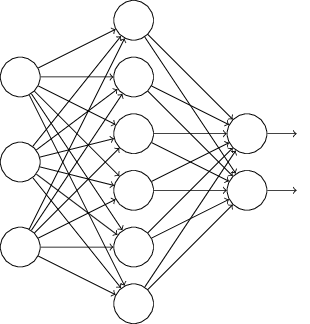
\includegraphics[width=0.9\textwidth]{images/tikz30.png}
\end{center}

\noindent 特别地，假设我们有一个训练输入 $x$ 和对应的期望输出 $y$. 通常，我们会通过将 $x$ 前馈传播通过网络来训练，然后反向传播以确定对梯度的贡献. 使用 dropout 时，这个过程被修改了. 我们首先随机地（并且暂时地）删除网络中一半的隐藏神经元，同时保持输入和输出神经元不变. 这样做之后，我们将得到一个大致如下的网络. 注意，被 dropout 的神经元，即那些被暂时删除的神经元，仍然以虚影显示：

\begin{center}
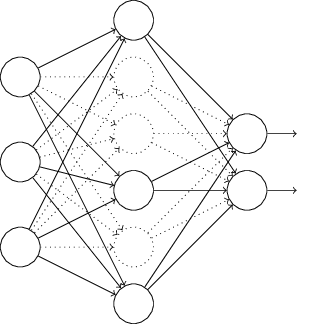
\includegraphics[width=0.9\textwidth]{images/tikz31.png}
\end{center}

\noindent 我们将输入 $x$ 通过修改后的网络前馈传播，然后将结果也通过修改后的网络反向传播. 在一个小批量的样本上这样做之后，我们更新相应的权重和偏置. 然后我们重复这个过程，首先恢复被 dropout 的神经元，然后选择一个新的随机隐藏神经元子集来删除，为另一个小批量估计梯度，并更新网络中的权重和偏置.

通过一遍又一遍地重复这个过程，我们的网络将学到一组权重和偏置. 当然，这些权重和偏置是在一半隐藏神经元被丢弃的条件下学到的. 当我们实际运行完整的网络时，这意味着将有两倍的隐藏神经元处于活跃状态. 为了补偿这一点，我们将从隐藏神经元输出的权重减半.

这个 dropout 过程可能看起来奇怪且\emph{临时拼凑}. 我们为什么会期望它有助于正则化呢？为了解释这是怎么回事，我希望你暂时停止思考 dropout，而是想象以标准方式（无 dropout）训练神经网络. 特别地，想象我们训练几个不同的神经网络，都使用相同的训练数据. 当然，这些网络可能一开始并不完全相同，因此训练后它们有时可能给出不同的结果. 当这种情况发生时，我们可以使用某种平均或投票方案来决定接受哪个输出. 例如，如果我们训练了五个网络，其中三个将某个数字分类为``3''，那么它很可能真的是``3''. 另外两个网络很可能只是犯了错误. 这种平均方案通常被发现是一种强大（尽管昂贵）的减少过拟合的方法. 原因是不同的网络可能以不同的方式过拟合，而平均可能有助于消除那种过拟合.

这与 dropout 有什么关系呢？启发式地说，当我们 dropout 不同的神经元集合时，这有点像我们在训练不同的神经网络. 因此，dropout 过程就像是对大量不同网络的效果进行平均. 不同的网络会以不同的方式过拟合，因此，希望 dropout 的净效果是减少过拟合.

在一篇最早使用该技术的论文*\footnote{ImageNet Classification with Deep Convolutional Neural Networks, by Alex Krizhevsky, Ilya Sutskever, and Geoffrey Hinton (2012).}中给出了一个相关的启发式解释：``This technique reduces complex co-adaptations of neurons, since a neuron cannot rely on the presence of particular other neurons. It is, therefore, forced to learn more robust features that are useful in conjunction with many different random subsets of the other neurons.'' 换句话说，如果我们把网络看作一个正在做出预测的模型，那么我们可以把 dropout 看作一种确保模型对丢失任何单个证据片段都具有鲁棒性的方法. 在这一点上，它有点类似于 L1 和 L2 正则化，后者倾向于减小权重，从而使网络对丢失网络中的任何单个连接更加鲁棒.

当然，dropout 的真正衡量标准是它在提高神经网络性能方面非常成功. 引入该技术的原始论文*\footnote{Improving neural networks by preventing co-adaptation of feature detectors by Geoffrey Hinton, Nitish Srivastava, Alex Krizhevsky, Ilya Sutskever, and Ruslan Salakhutdinov (2012). Note that the paper discusses a number of subtleties that I have glossed over in this brief introduction.}将其应用于许多不同的任务. 对我们来说，特别感兴趣的是他们将 dropout 应用于 MNIST 数字分类，使用了一个类似于我们一直在考虑的那种普通前馈神经网络. 论文指出，在此之前，使用这种架构所取得的最佳结果是在测试集上达到 $98.4$ ％的分类准确率. 他们使用 dropout 和一种修改形式的 L2 正则化的组合，将其提高到 $98.7$ ％的准确率. 在许多其他任务上也获得了类似令人印象深刻的结果，包括图像和语音识别以及自然语言处理中的问题. Dropout 在训练大型深度网络时特别有用，因为在这些网络中过拟合问题往往很严重. \textbf{人为地扩展训练数据：} 我们之前看到，当我们只使用 1,000 张训练图像时，我们的 MNIST 分类准确率下降到 80 ％多. 这并不奇怪，因为更少的训练数据意味着我们的网络将接触到更少的人类书写数字方式的变化. 让我们尝试用各种不同的训练数据集大小来训练我们的 30 个隐藏神经元网络，看看性能如何变化. 我们使用小批量大小 10、学习率 $\eta = 0.5$、正则化参数 $\lambda = 5.0$ 以及交叉熵代价函数进行训练. 当使用完整训练数据集时，我们将训练 30 个轮次，当使用较小的训练集时，我们将按比例增加轮次数量. 为了确保权重衰减因子在不同训练集之间保持一致，当使用完整训练数据集时，我们将使用正则化参数 $\lambda = 5.0$，当使用较小的训练集时，我们将按比例减小 $\lambda$*\footnote{This and the next two graph are produced with the program more\_\allowbreak{}data.py.}.

\begin{center}
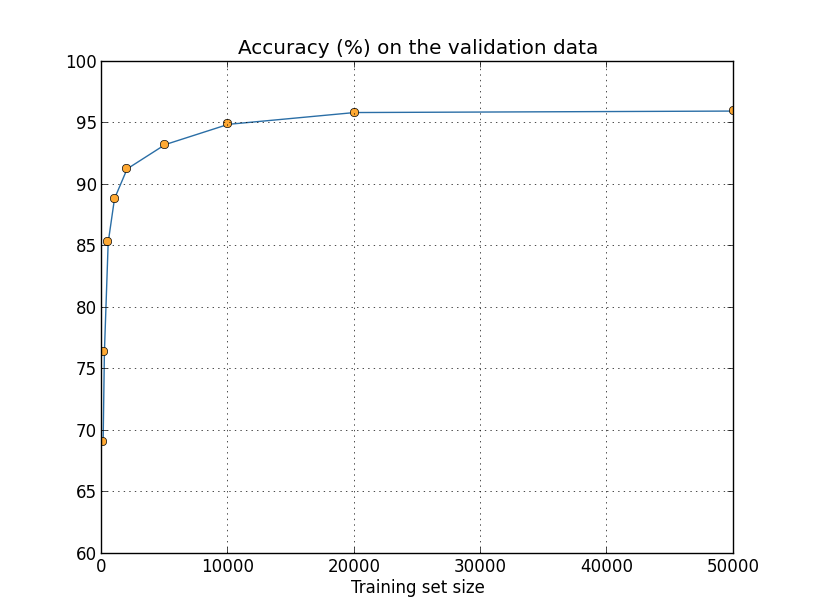
\includegraphics[width=0.867\textwidth]{images/more_data.png}
\end{center}

如你所见，随着我们使用更多的训练数据，分类准确率显著提高. 如果有更多数据可用，这种改进大概还会继续. 当然，看上面的图，确实看起来我们正在接近饱和. 然而，假设我们用对数坐标绘制训练集大小来重做这个图：

\begin{center}
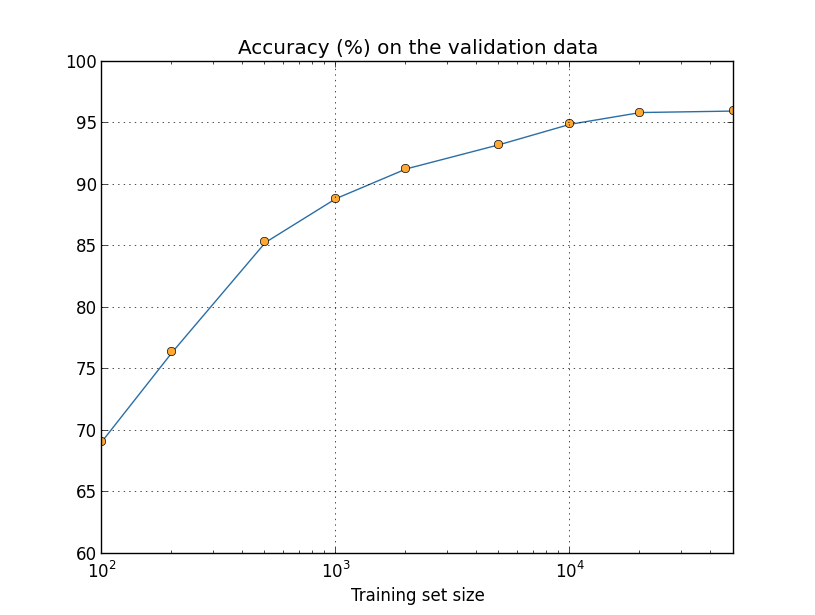
\includegraphics[width=0.867\textwidth]{images/more_data_log.png}
\end{center}

\noindent 很明显，图在末端仍在上升. 这表明，如果我们使用多得多的训练数据——比如说，数百万甚至数十亿个手写样本，而不仅仅是 50,000 个——那么我们很可能会获得相当好的性能，即使是从这个非常小的网络.

获取更多训练数据是个好主意. 不幸的是，这可能很昂贵，因此在实践中并不总是可行. 然而，还有另一个几乎同样有效的想法，那就是人为地扩展训练数据. 例如，假设我们取一张 MNIST 训练图像中的数字五，

\begin{center}
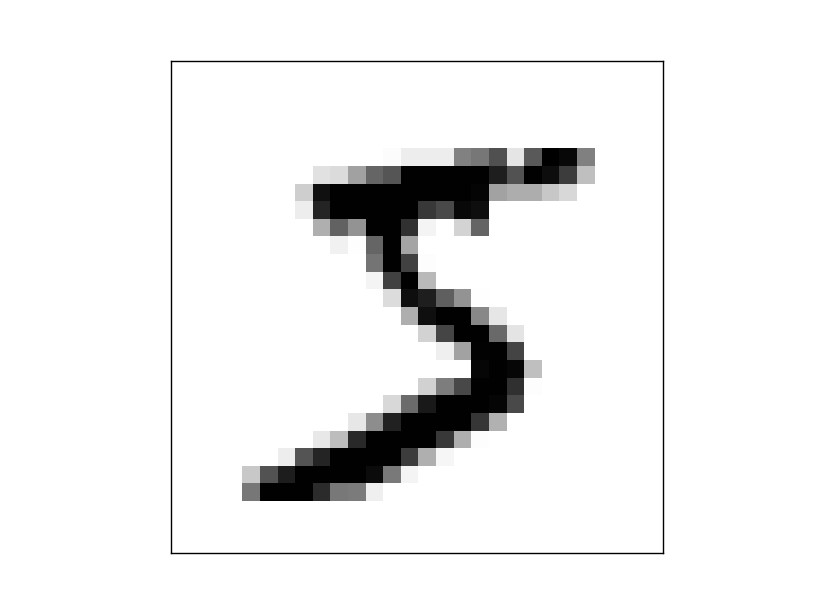
\includegraphics[width=0.200\textwidth]{images/more_data_5.png}
\end{center}

\noindent 并将其旋转一个小角度，比如说 15 度：

\begin{center}
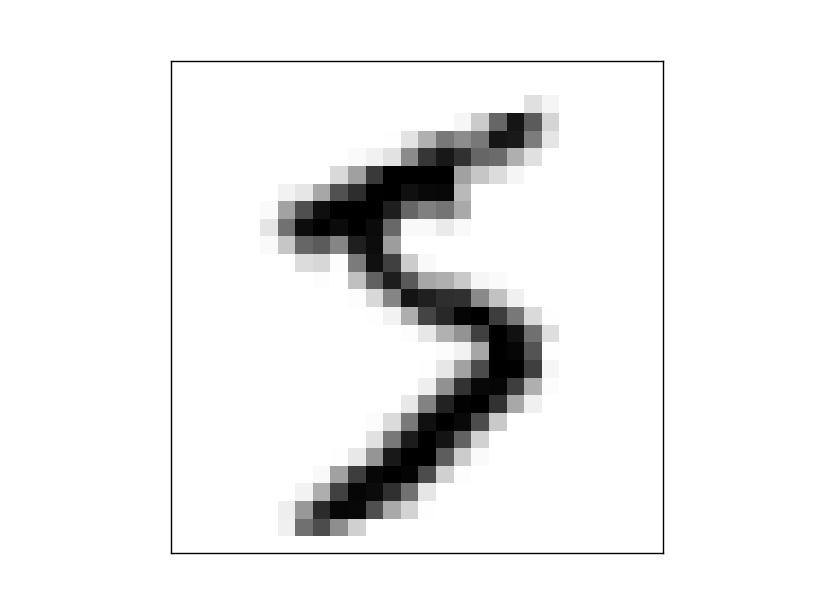
\includegraphics[width=0.200\textwidth]{images/more_data_rotated_5.png}
\end{center}

\noindent 它仍然可以识别为同一个数字. 然而在像素层面上，它与 MNIST 训练数据中当前的任何图像都相当不同. 可以想象，将这张图像添加到训练数据中可能有助于我们的网络学习更多关于如何分类数字的知识. 更重要的是，显然我们不仅限于添加这一张图像. 我们可以通过对\emph{所有} MNIST 训练图像进行\emph{许多}小的旋转来扩展我们的训练数据，然后使用扩展后的训练数据来提高我们网络的性能.
这个想法非常强大，并且已被广泛使用. 让我们看一篇论文* \footnote{Best Practices for Convolutional Neural Networks Applied to Visual Document Analysis, by Patrice Simard, Dave Steinkraus, and John Platt (2003).} 中的一些结果，该论文将这个想法的几种变体应用于 MNIST. 他们考虑的其中一种神经网络架构与我们一直在使用的类似，是一个具有 800 个隐藏神经元并使用交叉熵代价函数的前馈网络. 使用标准的 MNIST 训练数据运行该网络，他们在测试集上达到了 98.4\% 的分类准确率. 但随后他们扩展了训练数据，不仅使用了如我上文所述的旋转，还使用了平移和倾斜图像. 通过在扩展数据集上训练，他们将网络的准确率提高到了 98.9\%. 他们还实验了他们所谓的``弹性畸变''，这是一种特殊的图像畸变，旨在模拟手部肌肉中发现的随机振荡. 通过使用弹性畸变来扩展数据，他们获得了更高的准确率，99.3\%. 实际上，他们通过让网络接触到真实手写中存在的各种变化，拓宽了网络的经验.

这个想法的变体可用于提高许多学习任务的性能，而不仅仅是手写识别. 一般原则是通过应用反映真实世界变化的操作来扩展训练数据. 想出做到这一点的方法并不困难. 例如，假设你正在构建一个进行语音识别的神经网络. 我们人类即使在存在背景噪声等畸变的情况下也能识别语音. 因此，你可以通过添加背景噪声来扩展你的数据. 我们也能识别加速或减速的语音. 所以这是扩展训练数据的另一种方式. 这些技术并不总是被使用——例如，与其通过添加噪声来扩展训练数据，不如先应用降噪滤波器来清理网络的输入，这很可能更有效率. 尽管如此，将扩展训练数据的想法记在心中，并寻找机会应用它，是值得的.

\begin{exerciseBox}{练习}

\begin{itemize}

\item 如上所述，扩展 MNIST 训练数据的一种方法是使用训练图像的小角度旋转. 如果我们允许训练图像任意大角度的旋转，可能会出现什么问题？

\end{itemize}

\textbf{关于大数据以及比较分类准确率意味着什么的题外话：} 让我们再次审视我们的神经网络准确率如何随训练集大小变化：

\begin{center}
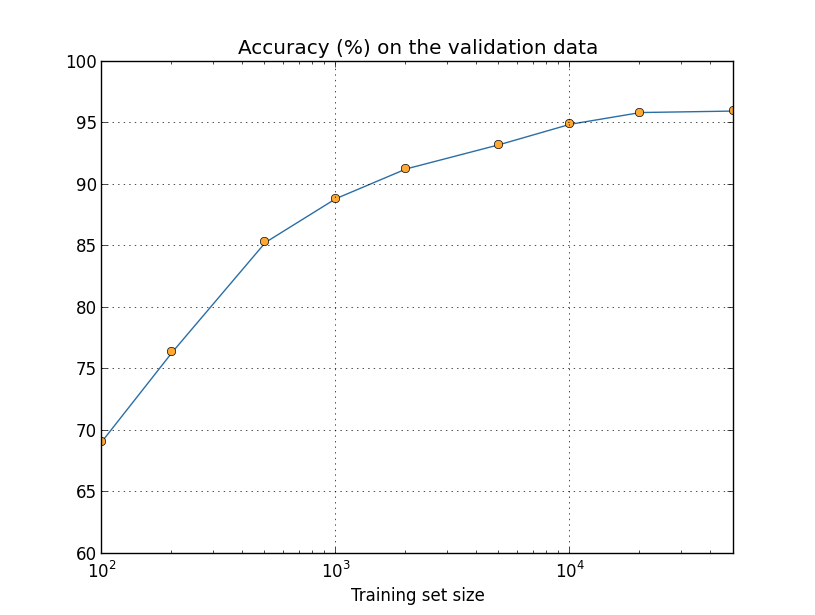
\includegraphics[width=0.867\textwidth]{images/more_data_log.png}
\end{center}

\noindent 假设我们不使用神经网络，而是使用其他一些机器学习技术来分类数字. 例如，让我们尝试使用我们在第 1 章简要介绍过的支持向量机（SVM）. 与第 1 章的情况一样，如果你不熟悉 SVM 也不用担心，我们不需要理解它们的细节. 相反，我们将使用 scikit-learn 库提供的 SVM. 下面是 SVM 性能随训练集大小变化的情况. 为了方便比较，我也绘制了神经网络的结果* \footnote{This graph was produced with the program more\_\allowbreak{}data.py (as were the last few graphs).}：

\begin{center}
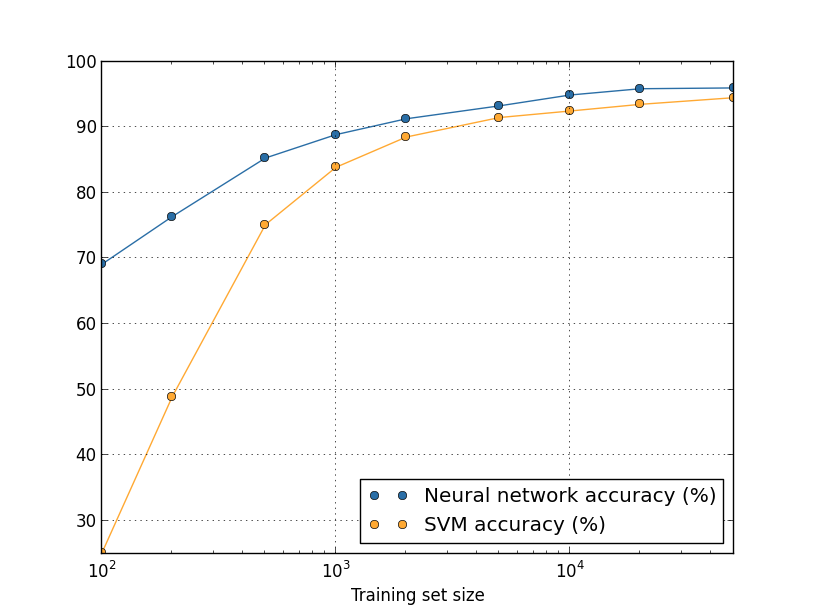
\includegraphics[width=0.867\textwidth]{images/more_data_comparison.png}
\end{center}

\noindent 关于这张图，可能首先让你注意到的是，对于每一种训练集大小，我们的神经网络都优于 SVM. 这很好，尽管你不应过度解读，因为我只是使用了 scikit-learn 的 SVM 的默认设置，而我们则做了相当多的工作来改进我们的神经网络. 关于这张图，一个更微妙但也更有趣的事实是，如果我们使用 50,000 张图像训练我们的 SVM，那么它的性能（94.48\% 准确率）实际上比我们的神经网络使用 5,000 张图像训练时的性能（93.24\% 准确率）更好. 换句话说，更多的训练数据有时可以弥补所使用的机器学习算法之间的差异.

甚至可能发生更有趣的事情. 假设我们试图使用两种机器学习算法，算法 A 和算法 B，来解决一个问题. 有时会发生算法 A 在一组训练数据上优于算法 B，而算法 B 在另一组不同的训练数据上优于算法 A 的情况. 我们在上面没有看到这种情况——那需要两条曲线交叉——但它确实会发生* \footnote{Striking examples may be found in Scaling to very very large corpora for natural language disambiguation, by Michele Banko and Eric Brill (2001).}. 对于问题``算法 A 比算法 B 更好吗？''，正确的回答实际上是：``你使用的是哪个训练数据集？''

所有这些都是需要牢记的警示，无论是在进行开发时，还是在阅读研究论文时. 许多论文专注于寻找新的技巧，以在标准基准数据集上榨取改进的性能.``我们的神奇技术使我们在标准基准 Y 上获得了 X\% 的提升''是研究声明的一种典型形式. 这类声明通常确实有趣，但必须理解为仅在所使用的特定训练数据集的背景下适用. 想象一个替代历史，在这个历史中，最初创建基准数据集的人获得了更多的研究经费. 他们可能会用这笔额外的钱来收集更多的训练数据. 那么，由神奇技术带来的``改进''完全有可能在更大的数据集上消失. 换句话说，所谓的改进可能只是历史的偶然. 要吸取的信息，尤其是在实际应用中，是我们既想要更好的算法\emph{也}想要更好的训练数据. 寻找更好的算法是好的，但要确保你没有只关注更好的算法，而忽略了获取更多或更好训练数据这些容易的胜利.

\end{exerciseBox}

\begin{exerciseBox}{习题}

\begin{itemize}

\item \textbf{（研究问题）} 我们的机器学习算法在非常大的数据集的极限情况下表现如何？对于任何给定的算法，很自然地会尝试在真正大数据的极限下定义渐近性能的概念. 解决这个问题的一个快速而粗略的方法是简单地尝试将曲线拟合到如上所示的图表，然后将拟合的曲线外推到无穷大. 这种方法的一个反对意见是，不同的曲线拟合方法会给出不同的渐近性能概念. 你能找到拟合到某个特定类别曲线的有原则的理由吗？如果能，请比较几种不同机器学习算法的渐近性能.

\end{itemize}

\textbf{总结：} 我们现在已经完成了对过拟合和正则化的深入探讨. 当然，我们还会再次回到这个问题. 正如我多次提到的，过拟合是神经网络中的一个主要问题，尤其是随着计算机变得更加强大，我们有能力训练更大的网络. 因此，迫切需要开发强大的正则化技术来减少过拟合，这是一个当前极其活跃的研究领域.

\end{exerciseBox}
\sectionTitle{权重初始化}{权重初始化}

当我们创建神经网络时，我们必须为初始权重和偏置做出选择. 到目前为止，我们一直按照我在第 1 章中简要讨论过的一个方案来选择它们. 提醒一下，那个方案是使用独立的高斯随机变量来选择权重和偏置，并归一化为均值为 $0$、标准差为 $1$. 虽然这种方法效果不错，但它相当 \emph{ad hoc}，值得重新审视，看看我们能否找到一种更好的方式来设置初始权重和偏置，或许还能帮助我们的神经网络学得更快.

事实证明，我们可以做得比用归一化高斯分布初始化好得多. 要理解原因，假设我们正在处理一个具有大量输入神经元的网络——比如 $1,000$ 个. 再假设我们使用了归一化高斯分布来初始化连接到第一个隐藏层的权重. 现在我将专门关注连接输入神经元到隐藏层中第一个神经元的权重，忽略网络的其余部分：

\begin{center}
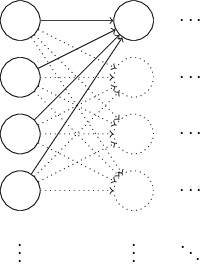
\includegraphics[width=0.9\textwidth]{images/tikz32.png}
\end{center}

\noindent 为简单起见，我们假设正在使用一个训练输入 $x$ 进行训练，其中一半的输入神经元是开启的，即设为 $1$，一半的输入神经元是关闭的，即设为 $0$. 接下来的论证更普遍地适用，但你会从这个特例中领会到要点. 让我们考虑隐藏神经元的输入的加权和 $z = \sum_j w_j x_j+b$. 这个和中有 $500$ 项消失了，因为对应的输入 $x_j$ 为零. 因此 $z$ 是总共 $501$ 个归一化高斯随机变量之和，包括 $500$ 个权重项和 $1$ 个额外的偏置项. 于是 $z$ 本身服从均值为零、标准差为 $\sqrt{501} \approx 22.4$ 的高斯分布. 也就是说，$z$ 具有非常宽的高斯分布，完全不是尖锐的峰值：特别地，我们可以从这个图中看到，$|z|$ 很可能会相当大，即要么 $z \gg 1$ 要么 $z \ll -1$. 如果是这种情况，那么隐藏神经元的输出 $\sigma(z)$ 将非常接近 $1$ 或 $0$. 这意味着我们的隐藏神经元将饱和. 当这种情况发生时，正如我们所知，对权重做微小改变只会对隐藏神经元的激活值产生极其微小的变化. 隐藏神经元激活值的这种微小变化反过来几乎完全不会影响网络中其余的神经元，我们也会看到代价函数相应地只有极其微小的变化. 结果，当我们使用梯度下降算法时，那些权重只会学习得非常慢*\footnote{我们在第 2 章中更详细地讨论了这一点，在那里我们使用反向传播方程来表明输入到饱和神经元的权重学习得很慢.}. 这类似于我们在本章前面讨论过的问题，即输出神经元在错误的值上饱和导致学习减慢. 我们通过巧妙选择代价函数解决了前面那个问题. 不幸的是，虽然那对饱和的输出神经元有帮助，但对饱和的隐藏神经元的问题完全无济于事.

我一直在谈论输入到第一个隐藏层的权重. 当然，类似的论证也适用于后面的隐藏层：如果后面隐藏层的权重使用归一化高斯分布初始化，那么激活值往往会非常接近 $0$ 或 $1$，学习将进行得非常缓慢.

有没有什么方法可以为权重和偏置选择更好的初始化，从而不会出现这种饱和，避免学习减慢？假设我们有一个具有 $n_{\rm in}$ 个输入权重的神经元. 那么我们将这些权重初始化为均值为 $0$、标准差为 $1/\sqrt{n_{\rm in}}$ 的高斯随机变量. 也就是说，我们将高斯分布压缩，使得我们的神经元不太可能饱和. 我们将继续把偏置选择为均值为 $0$、标准差为 $1$ 的高斯分布，原因我稍后会再谈. 有了这些选择，加权和 $z = \sum_j w_j x_j + b$ 将再次是一个均值为 $0$ 的高斯随机变量，但它会比之前尖锐得多. 假设像之前一样，$500$ 个输入为零，$500$ 个输入为 $1$. 那么很容易证明（见下面的练习）$z$ 服从均值为 $0$、标准差为 $\sqrt{3/2} = 1.22\ldots$ 的高斯分布. 这比之前尖锐得多，以至于下面的图甚至低估了这种情况，因为与之前的图相比，我不得不重新调整了纵轴的比例：这样的神经元饱和的可能性要小得多，相应地出现学习减慢问题的可能性也小得多.

\begin{exerciseBox}{练习}

\begin{itemize}

\item 验证上面段落中 $z = \sum_j w_j x_j + b$ 的标准差是 $\sqrt{3/2}$. 知道以下事实可能有帮助：(a) 独立随机变量之和的方差是各个随机变量方差之和；(b) 方差是标准差的平方.

\end{itemize}

我上面说过我们将像之前一样继续初始化偏置，即作为均值为 $0$、标准差为 $1$ 的高斯随机变量. 这是可以的，因为它不会使我们的神经元饱和的可能性增加太多. 事实上，我们如何初始化偏置并不太重要，只要避免饱和问题即可. 有些人甚至将所有偏置初始化为 $0$，依靠梯度下降来学习合适的偏置. 但由于这不太可能产生太大差异，我们将继续使用与之前相同的初始化过程.

让我们使用 MNIST 数字分类任务来比较新旧两种权重初始化方法的结果. 和之前一样，我们将使用 $30$ 个隐藏神经元、小批量大小为 $10$、正则化参数 $\lambda = 5.0$ 以及交叉熵代价函数. 我们将学习率从 $\eta = 0.5$ 略微降低到 $0.1$，因为这使结果在图中更容易看清. 我们可以使用旧的权重初始化方法进行训练：

\begin{lstlisting}
>>> import mnist_loader
>>> training_data, validation_data, test_data = \
... mnist_loader.load_data_wrapper()
>>> import network2
>>> net = network2.Network([784, 30, 10], cost=network2.CrossEntropyCost)
>>> net.large_weight_initializer()
>>> net.SGD(training_data, 30, 10, 0.1, lmbda = 5.0,
... evaluation_data=validation_data,
... monitor_evaluation_accuracy=True)

\end{lstlisting}

我们也可以使用新的权重初始化方法进行训练. 这实际上更容易，因为 network2 默认的权重初始化方式就是使用这种新方法. 这意味着我们可以省略上面的 net.large\_\allowbreak{}weight\_\allowbreak{}initializer() 调用：

\begin{lstlisting}
>>> net = network2.Network([784, 30, 10], cost=network2.CrossEntropyCost)
>>> net.SGD(training_data, 30, 10, 0.1, lmbda = 5.0,
... evaluation_data=validation_data,
... monitor_evaluation_accuracy=True)

\end{lstlisting}

绘制结果* *用于生成这张图和下一张图的程序是 weight\_\allowbreak{}initialization.py.

，我们得到：

\begin{center}
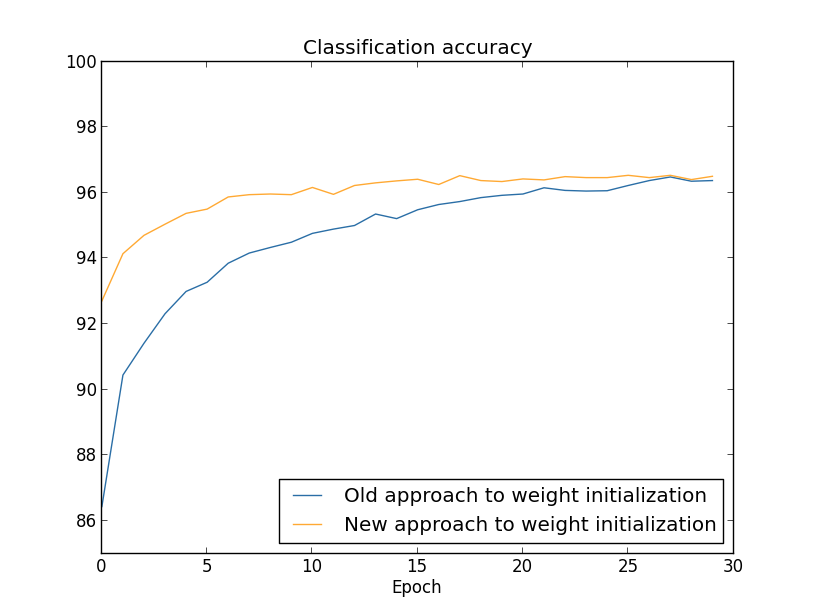
\includegraphics[width=0.867\textwidth]{images/weight_initialization_30.png}
\end{center}

\noindent 在两种情况下，我们最终得到的分类准确率都略高于 96\%. 最终的分类准确率在两种情况下几乎完全相同. 但新的初始化技术让我们更快、快得多地达到那里. 在第一个训练轮次结束时，旧的权重初始化方法的分类准确率不到 87\%，而新方法已经接近 93\%. 看起来正在发生的是，我们新的权重初始化方法让我们从一个好得多的状态开始，这使我们能够更快地获得好的结果. 如果我们用 $100$ 个隐藏神经元绘制结果，也会看到同样的现象：

\begin{center}
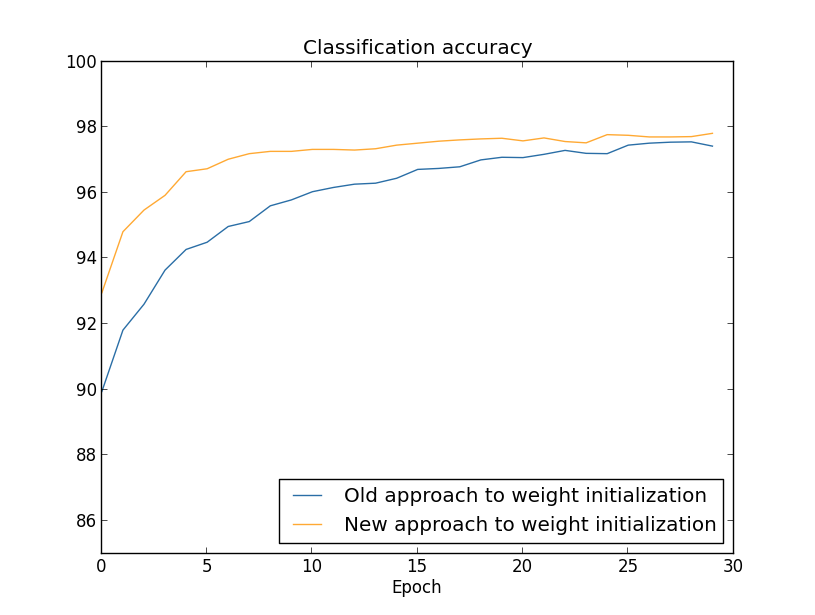
\includegraphics[width=0.867\textwidth]{images/weight_initialization_100.png}
\end{center}

\noindent 在这种情况下，两条曲线没有完全重合. 然而，我的实验表明，只需再训练几个轮次（未显示），准确率就会变得几乎完全相同. 因此，基于这些实验，看起来改进的权重初始化只是加速了学习，并没有改变我们网络的最终性能. 然而，在第 4 章中我们将看到一些神经网络的例子，其中长期行为在使用 $1/\sqrt{n_{\rm in}}$ 权重初始化时显著更好. 因此，不仅学习速度得到了改善，有时最终性能也得到了改善.

$1/\sqrt{n_{\rm in}}$ 权重初始化方法有助于改善我们神经网络的学习方式. 其他权重初始化技术也被提出过，许多都建立在这个基本思想之上. 我不会在这里回顾其他方法，因为 $1/\sqrt{n_{\rm in}}$ 对我们的目的来说已经足够好了. 如果你有兴趣进一步了解，我推荐看看 Yoshua Bengio 2012 年论文第 14 和 15 页的讨论*\footnote{Practical Recommendations for Gradient-Based Training of Deep Architectures, by Yoshua Bengio (2012).}，以及其中的参考文献.

\end{exerciseBox}

\begin{exerciseBox}{习题}

\begin{itemize}

\item \textbf{将正则化与改进的权重初始化方法联系起来} L2 正则化有时会自动给我们类似于新权重初始化方法的东西. 假设我们正在使用旧的权重初始化方法. 草拟一个启发式论证：(1) 假设 $\lambda$ 不太小，最初的几个训练轮次将几乎完全由权重衰减主导；(2) 只要 $\eta \lambda \ll n$，权重每轮次将按因子 $\exp(-\eta \lambda / m)$ 衰减；(3) 假设 $\lambda$ 不太大，当权重降到大约 $1/\sqrt{n}$ 的大小时，权重衰减将逐渐减弱，其中 $n$ 是网络中权重的总数. 论证这些条件在本节所绘制的例子中都得到了满足.

\end{itemize}

\end{exerciseBox}
\sectionTitle{重访手写数字识别：代码}{重访手写数字识别：代码}

让我们来实现本章中讨论过的想法. 我们将开发一个新程序 \texttt{network2.py}，它是我们在第 1 章中开发的程序 \texttt{network.py} 的改进版本. 如果你有一阵子没看过 \texttt{network.py} 了，那么花几分钟快速重读一下之前的讨论可能会对你有所帮助. 它只有 74 行代码，很容易理解.

和 \texttt{network.py} 中的情况一样，\texttt{network2.py} 的主角是 \texttt{Network} 类，我们用它来表示我们的神经网络. 我们用一个包含网络中各个层 \texttt{sizes} 的列表，以及一个要使用的 \texttt{cost} 选择来初始化 \texttt{Network} 的一个实例，默认使用交叉熵：

\begin{lstlisting}
class Network(object):

    def __init__(self, sizes, cost=CrossEntropyCost):
        self.num_layers = len(sizes)
        self.sizes = sizes
        self.default_weight_initializer()
        self.cost=cost

\end{lstlisting}

\texttt{\_\allowbreak{}\_\allowbreak{}init\_\allowbreak{}\_\allowbreak{}} 方法的前几行与 \texttt{network.py} 中相同，而且相当不言自明. 但接下来的两行是新的，我们需要详细理解它们在做什么.

让我们从考察 \texttt{default\_\allowbreak{}weight\_\allowbreak{}initializer} 方法开始. 它利用了我们新的、改进过的权重初始化方法. 正如我们所见，在该方法中，输入到一个神经元的权重被初始化为均值为 0、标准差为 $1$ 除以输入到该神经元的连接数的平方根的高斯随机变量. 同样在这个方法中，我们将初始化偏置，使用均值为 $0$、标准差为 $1$ 的高斯随机变量. 代码如下：

\begin{lstlisting}
    def default_weight_initializer(self):
        self.biases = [np.random.randn(y, 1) for y in self.sizes[1:]]
        self.weights = [np.random.randn(y, x)/np.sqrt(x)
                        for x, y in zip(self.sizes[:-1], self.sizes[1:])]

\end{lstlisting}

要理解这段代码，回忆一下 \texttt{np} 是用于进行线性代数的 Numpy 库可能会有所帮助. 我们会在程序开头 \texttt{import} Numpy. 另外，注意我们没有为第一层神经元初始化任何偏置. 我们避免这样做是因为第一层是输入层，因此任何偏置都不会被用到. 我们在 \texttt{network.py} 中做的完全一样.

作为 \texttt{default\_\allowbreak{}weight\_\allowbreak{}initializer} 的补充，我们还会包含一个 \texttt{large\_\allowbreak{}weight\_\allowbreak{}initializer} 方法. 这个方法使用第 1 章中的旧方法初始化权重和偏置，将权重和偏置都初始化为均值为 $0$、标准差为 $1$ 的高斯随机变量. 当然，这段代码与 \texttt{default\_\allowbreak{}weight\_\allowbreak{}initializer} 只有一点点不同：

\begin{lstlisting}
    def large_weight_initializer(self):
        self.biases = [np.random.randn(y, 1) for y in self.sizes[1:]]
        self.weights = [np.random.randn(y, x)
                        for x, y in zip(self.sizes[:-1], self.sizes[1:])]

\end{lstlisting}

我包含 \texttt{large\_\allowbreak{}weight\_\allowbreak{}initializer} 方法主要是为了方便，使本章的结果更容易与第 1 章的结果进行比较. 我想不出有多少实际情形会让我推荐使用它！

\texttt{Network} 的 \texttt{\_\allowbreak{}\_\allowbreak{}init\_\allowbreak{}\_\allowbreak{}} 方法中的第二个新事物是我们现在初始化了一个 \texttt{cost} 属性. 要理解它是如何工作的，让我们看看我们用来表示交叉熵代价的类*\footnote{如果你不熟悉 Python 的静态方法，你可以忽略 \texttt{@staticmethod} 装饰器，只把 \texttt{fn} 和 \texttt{delta} 当作普通方法即可. 如果你对细节感到好奇，\texttt{@staticmethod} 所做的只是告诉 Python 解释器，紧随其后的方法不以任何方式依赖于对象. 这就是为什么 \texttt{self} 没有作为参数传递给 \texttt{fn} 和 \texttt{delta} 方法.}：

\begin{lstlisting}
class CrossEntropyCost(object):

    @staticmethod
    def fn(a, y):
        return np.sum(np.nan_to_num(-y*np.log(a)-(1-y)*np.log(1-a)))

    @staticmethod
    def delta(z, a, y):
        return (a-y)

\end{lstlisting}

让我们来分解一下. 首先要观察到的是，尽管从数学上说交叉熵是一个函数，但我们把它实现为一个 Python 类，而不是一个 Python 函数. 我为什么做出这个选择？原因是代价在我们的网络中扮演两种不同的角色. 显而易见的角色是，它是输出激活值 \texttt{a} 与期望输出 \texttt{y} 匹配程度的度量. 这个角色由 \texttt{CrossEntropyCost.fn} 方法承担. （顺便注意，\texttt{CrossEntropyCost.fn} 内部的 \texttt{np.nan\_\allowbreak{}to\_\allowbreak{}num} 调用确保 Numpy 正确处理非常接近于零的数的对数.）但代价函数进入我们网络还有第二种方式. 回忆第 2 章，在运行反向传播算法时，我们需要计算网络的输出误差 $\delta^L$. 输出误差的形式取决于代价函数的选择：不同的代价函数，输出误差的形式不同. 对于交叉熵，输出误差正如我们在公式 (66) 中所见

\begin{align*}
\delta^L = a^L-y. \nonumber
\end{align*}

\noindent，

\begin{equation}
\delta^L = a^L-y.
\tag{99}
\end{equation}

\noindent 出于这个原因，我们定义了第二个方法 \texttt{CrossEntropyCost.delta}，其目的是告诉我们的网络如何计算输出误差. 然后我们把这两个方法打包进一个单独的类中，其中包含我们的网络需要知道的关于代价函数的一切.

以类似的方式，\texttt{network2.py} 还包含一个表示二次代价函数的类. 包含它是为了与第 1 章的结果进行比较，因为往后我们将主要使用交叉熵. 代码就在下面. \texttt{QuadraticCost.fn} 方法是对与实际输出 \texttt{a} 和期望输出 \texttt{y} 相关联的二次代价的直接计算. \texttt{QuadraticCost.delta} 返回的值基于表达式 (30)

\begin{align*}
\delta^L = (a^L-y) \odot \sigma'(z^L) \nonumber
\end{align*}

\noindent 即二次代价的输出误差，这是我们在第 2 章中推导出来的.

\begin{lstlisting}
class QuadraticCost(object):

    @staticmethod
    def fn(a, y):
        return 0.5*np.linalg.norm(a-y)**2

    @staticmethod
    def delta(z, a, y):
        return (a-y) * sigmoid_prime(z)

\end{lstlisting}

我们现在已经理解了 \texttt{network2.py} 与 \texttt{network.py} 之间的主要区别. 全都是相当简单的东西. 还有一些较小的改动，我将在下面讨论，包括 L2 正则化的实现. 在讨论这些之前，让我们看看 \texttt{network2.py} 的完整代码. 你不需要详细阅读所有代码，但值得理解其大致结构，尤其是阅读文档字符串，这样你就能理解程序的每一部分在做什么. 当然，也欢迎你按自己的意愿深入钻研！如果你迷失了方向，不妨继续阅读下面的正文，稍后再回到代码. 总之，代码如下：

\begin{lstlisting}
"""network2.py
~~~~~~~~~~~~~~

An improved version of network.py, implementing the stochastic
gradient descent learning algorithm for a feedforward neural network.
Improvements include the addition of the cross-entropy cost function,
regularization, and better initialization of network weights.  Note
that I have focused on making the code simple, easily readable, and
easily modifiable.  It is not optimized, and omits many desirable
features.

"""

#### Libraries
# Standard library
import json
import random
import sys

# Third-party libraries
import numpy as np

#### Define the quadratic and cross-entropy cost functions

class QuadraticCost(object):

    @staticmethod
    def fn(a, y):
        """Return the cost associated with an output ``a`` and desired output
        ``y``.

        """
        return 0.5*np.linalg.norm(a-y)**2

    @staticmethod
    def delta(z, a, y):
        """Return the error delta from the output layer."""
        return (a-y) * sigmoid_prime(z)

class CrossEntropyCost(object):

    @staticmethod
    def fn(a, y):
        """Return the cost associated with an output ``a`` and desired output
        ``y``.  Note that np.nan_to_num is used to ensure numerical
        stability.  In particular, if both ``a`` and ``y`` have a 1.0
        in the same slot, then the expression (1-y)*np.log(1-a)
        returns nan.  The np.nan_to_num ensures that that is converted
        to the correct value (0.0).

        """
        return np.sum(np.nan_to_num(-y*np.log(a)-(1-y)*np.log(1-a)))

    @staticmethod
    def delta(z, a, y):
        """Return the error delta from the output layer.  Note that the
        parameter ``z`` is not used by the method.  It is included in
        the method's parameters in order to make the interface
        consistent with the delta method for other cost classes.

        """
        return (a-y)

#### Main Network class
class Network(object):

    def __init__(self, sizes, cost=CrossEntropyCost):
        """The list ``sizes`` contains the number of neurons in the respective
        layers of the network.  For example, if the list was [2, 3, 1]
        then it would be a three-layer network, with the first layer
        containing 2 neurons, the second layer 3 neurons, and the
        third layer 1 neuron.  The biases and weights for the network
        are initialized randomly, using
        ``self.default_weight_initializer`` (see docstring for that
        method).

        """
        self.num_layers = len(sizes)
        self.sizes = sizes
        self.default_weight_initializer()
        self.cost=cost

    def default_weight_initializer(self):
        """Initialize each weight using a Gaussian distribution with mean 0
        and standard deviation 1 over the square root of the number of
        weights connecting to the same neuron.  Initialize the biases
        using a Gaussian distribution with mean 0 and standard
        deviation 1.

        Note that the first layer is assumed to be an input layer, and
        by convention we won't set any biases for those neurons, since
        biases are only ever used in computing the outputs from later
        layers.

        """
        self.biases = [np.random.randn(y, 1) for y in self.sizes[1:]]
        self.weights = [np.random.randn(y, x)/np.sqrt(x)
                        for x, y in zip(self.sizes[:-1], self.sizes[1:])]

    def large_weight_initializer(self):
        """Initialize the weights using a Gaussian distribution with mean 0
        and standard deviation 1.  Initialize the biases using a
        Gaussian distribution with mean 0 and standard deviation 1.

        Note that the first layer is assumed to be an input layer, and
        by convention we won't set any biases for those neurons, since
        biases are only ever used in computing the outputs from later
        layers.

        This weight and bias initializer uses the same approach as in
        Chapter 1, and is included for purposes of comparison.  It
        will usually be better to use the default weight initializer
        instead.

        """
        self.biases = [np.random.randn(y, 1) for y in self.sizes[1:]]
        self.weights = [np.random.randn(y, x)
                        for x, y in zip(self.sizes[:-1], self.sizes[1:])]

    def feedforward(self, a):
        """Return the output of the network if ``a`` is input."""
        for b, w in zip(self.biases, self.weights):
            a = sigmoid(np.dot(w, a)+b)
        return a

    def SGD(self, training_data, epochs, mini_batch_size, eta,
            lmbda = 0.0,
            evaluation_data=None,
            monitor_evaluation_cost=False,
            monitor_evaluation_accuracy=False,
            monitor_training_cost=False,
            monitor_training_accuracy=False):
        """Train the neural network using mini-batch stochastic gradient
        descent.  The ``training_data`` is a list of tuples ``(x, y)``
        representing the training inputs and the desired outputs.  The
        other non-optional parameters are self-explanatory, as is the
        regularization parameter ``lmbda``.  The method also accepts
        ``evaluation_data``, usually either the validation or test
        data.  We can monitor the cost and accuracy on either the
        evaluation data or the training data, by setting the
        appropriate flags.  The method returns a tuple containing four
        lists: the (per-epoch) costs on the evaluation data, the
        accuracies on the evaluation data, the costs on the training
        data, and the accuracies on the training data.  All values are
        evaluated at the end of each training epoch.  So, for example,
        if we train for 30 epochs, then the first element of the tuple
        will be a 30-element list containing the cost on the
        evaluation data at the end of each epoch. Note that the lists
        are empty if the corresponding flag is not set.

        """
        if evaluation_data: n_data = len(evaluation_data)
        n = len(training_data)
        evaluation_cost, evaluation_accuracy = [], []
        training_cost, training_accuracy = [], []
        for j in xrange(epochs):
            random.shuffle(training_data)
            mini_batches = [
                training_data[k:k+mini_batch_size]
                for k in xrange(0, n, mini_batch_size)]
            for mini_batch in mini_batches:
                self.update_mini_batch(
                    mini_batch, eta, lmbda, len(training_data))
            print "Epoch
            if monitor_training_cost:
                cost = self.total_cost(training_data, lmbda)
                training_cost.append(cost)
                print "Cost on training data: {}".format(cost)
            if monitor_training_accuracy:
                accuracy = self.accuracy(training_data, convert=True)
                training_accuracy.append(accuracy)
                print "Accuracy on training data: {} / {}".format(
                    accuracy, n)
            if monitor_evaluation_cost:
                cost = self.total_cost(evaluation_data, lmbda, convert=True)
                evaluation_cost.append(cost)
                print "Cost on evaluation data: {}".format(cost)
            if monitor_evaluation_accuracy:
                accuracy = self.accuracy(evaluation_data)
                evaluation_accuracy.append(accuracy)
                print "Accuracy on evaluation data: {} / {}".format(
                    self.accuracy(evaluation_data), n_data)
            print
        return evaluation_cost, evaluation_accuracy, \
            training_cost, training_accuracy

    def update_mini_batch(self, mini_batch, eta, lmbda, n):
        """Update the network's weights and biases by applying gradient
        descent using backpropagation to a single mini batch.  The
        ``mini_batch`` is a list of tuples ``(x, y)``, ``eta`` is the
        learning rate, ``lmbda`` is the regularization parameter, and
        ``n`` is the total size of the training data set.

        """
        nabla_b = [np.zeros(b.shape) for b in self.biases]
        nabla_w = [np.zeros(w.shape) for w in self.weights]
        for x, y in mini_batch:
            delta_nabla_b, delta_nabla_w = self.backprop(x, y)
            nabla_b = [nb+dnb for nb, dnb in zip(nabla_b, delta_nabla_b)]
            nabla_w = [nw+dnw for nw, dnw in zip(nabla_w, delta_nabla_w)]
        self.weights = [(1-eta*(lmbda/n))*w-(eta/len(mini_batch))*nw
                        for w, nw in zip(self.weights, nabla_w)]
        self.biases = [b-(eta/len(mini_batch))*nb
                       for b, nb in zip(self.biases, nabla_b)]

    def backprop(self, x, y):
        """Return a tuple ``(nabla_b, nabla_w)`` representing the
        gradient for the cost function C_x.  ``nabla_b`` and
        ``nabla_w`` are layer-by-layer lists of numpy arrays, similar
        to ``self.biases`` and ``self.weights``."""
        nabla_b = [np.zeros(b.shape) for b in self.biases]
        nabla_w = [np.zeros(w.shape) for w in self.weights]
        # feedforward
        activation = x
        activations = [x] # list to store all the activations, layer by layer
        zs = [] # list to store all the z vectors, layer by layer
        for b, w in zip(self.biases, self.weights):
            z = np.dot(w, activation)+b
            zs.append(z)
            activation = sigmoid(z)
            activations.append(activation)
        # backward pass
        delta = (self.cost).delta(zs[-1], activations[-1], y)
        nabla_b[-1] = delta
        nabla_w[-1] = np.dot(delta, activations[-2].transpose())
        # Note that the variable l in the loop below is used a little
        # differently to the notation in Chapter 2 of the book.  Here,
        # l = 1 means the last layer of neurons, l = 2 is the
        # second-last layer, and so on.  It's a renumbering of the
        # scheme in the book, used here to take advantage of the fact
        # that Python can use negative indices in lists.
        for l in xrange(2, self.num_layers):
            z = zs[-l]
            sp = sigmoid_prime(z)
            delta = np.dot(self.weights[-l+1].transpose(), delta) * sp
            nabla_b[-l] = delta
            nabla_w[-l] = np.dot(delta, activations[-l-1].transpose())
        return (nabla_b, nabla_w)

    def accuracy(self, data, convert=False):
        """Return the number of inputs in ``data`` for which the neural
        network outputs the correct result. The neural network's
        output is assumed to be the index of whichever neuron in the
        final layer has the highest activation.

        The flag ``convert`` should be set to False if the data set is
        validation or test data (the usual case), and to True if the
        data set is the training data. The need for this flag arises
        due to differences in the way the results ``y`` are
        represented in the different data sets.  In particular, it
        flags whether we need to convert between the different
        representations.  It may seem strange to use different
        representations for the different data sets.  Why not use the
        same representation for all three data sets?  It's done for
        efficiency reasons -- the program usually evaluates the cost
        on the training data and the accuracy on other data sets.
        These are different types of computations, and using different
        representations speeds things up.  More details on the
        representations can be found in
        mnist_loader.load_data_wrapper.

        """
        if convert:
            results = [(np.argmax(self.feedforward(x)), np.argmax(y))
                       for (x, y) in data]
        else:
            results = [(np.argmax(self.feedforward(x)), y)
                        for (x, y) in data]
        return sum(int(x == y) for (x, y) in results)

    def total_cost(self, data, lmbda, convert=False):
        """Return the total cost for the data set ``data``.  The flag
        ``convert`` should be set to False if the data set is the
        training data (the usual case), and to True if the data set is
        the validation or test data.  See comments on the similar (but
        reversed) convention for the ``accuracy`` method, above.
        """
        cost = 0.0
        for x, y in data:
            a = self.feedforward(x)
            if convert: y = vectorized_result(y)
            cost += self.cost.fn(a, y)/len(data)
        cost += 0.5*(lmbda/len(data))*sum(
            np.linalg.norm(w)**2 for w in self.weights)
        return cost

    def save(self, filename):
        """Save the neural network to the file ``filename``."""
        data = {"sizes": self.sizes,
                "weights": [w.tolist() for w in self.weights],
                "biases": [b.tolist() for b in self.biases],
                "cost": str(self.cost.__name__)}
        f = open(filename, "w")
        json.dump(data, f)
        f.close()

#### Loading a Network
def load(filename):
    """Load a neural network from the file ``filename``.  Returns an
    instance of Network.

    """
    f = open(filename, "r")
    data = json.load(f)
    f.close()
    cost = getattr(sys.modules[__name__], data["cost"])
    net = Network(data["sizes"], cost=cost)
    net.weights = [np.array(w) for w in data["weights"]]
    net.biases = [np.array(b) for b in data["biases"]]
    return net

#### Miscellaneous functions
def vectorized_result(j):
    """Return a 10-dimensional unit vector with a 1.0 in the j'th position
    and zeroes elsewhere.  This is used to convert a digit (0...9)
    into a corresponding desired output from the neural network.

    """
    e = np.zeros((10, 1))
    e[j] = 1.0
    return e

def sigmoid(z):
    """The sigmoid function."""
    return 1.0/(1.0+np.exp(-z))

def sigmoid_prime(z):
    """Derivative of the sigmoid function."""
    return sigmoid(z)*(1-sigmoid(z))

\end{lstlisting}
代码中比较有趣的一个变化是加入了 L2 正则化. 虽然这是一个概念上的重大改变，但实现起来却微不足道，以至于在代码中很容易被忽略. 大部分情况下，它只是把参数 \texttt{lmbda} 传给各种方法，尤其是 \texttt{Network.SGD} 方法. 真正的工作由程序中的一行完成，即 \texttt{Network.update\_\allowbreak{}mini\_\allowbreak{}batch} 方法的倒数第四行. 正是在那里，我们修改了梯度下降的更新规则以包含权重衰减. 但尽管这个修改很小，它对结果却有巨大的影响！

顺便说一句，在神经网络中实现新技术时，这是很常见的. 我们花了数千字讨论正则化. 它在概念上相当微妙且难以理解. 然而把它加入我们的程序却是微不足道的！复杂的技术可以通过对代码的小改动来实现，这种情况出奇地常见.

我们代码中另一个小而重要的改动是给随机梯度下降方法 \texttt{Network.SGD} 增加了几个可选标志. 这些标志使得我们可以监控 \texttt{training\_\allowbreak{}data} 上的代价和准确率，或者监控可以传给 \texttt{Network.SGD} 的一组 \texttt{evaluation\_\allowbreak{}data} 上的代价和准确率. 我们在本章前面已经多次使用过这些标志，但让我举一个例子说明它是如何工作的，只是为了提醒你一下：

\begin{lstlisting}
>>> import mnist_loader
>>> training_data, validation_data, test_data = \
... mnist_loader.load_data_wrapper()
>>> import network2
>>> net = network2.Network([784, 30, 10], cost=network2.CrossEntropyCost)
>>> net.SGD(training_data, 30, 10, 0.5,
... lmbda = 5.0,
... evaluation_data=validation_data,
... monitor_evaluation_accuracy=True,
... monitor_evaluation_cost=True,
... monitor_training_accuracy=True,
... monitor_training_cost=True)

\end{lstlisting}

这里，我们把 \texttt{evaluation\_\allowbreak{}data} 设为 \texttt{validation\_\allowbreak{}data}. 但我们也可以监控 \texttt{test\_\allowbreak{}data} 或任何其他数据集上的性能. 我们还有四个标志，告诉我们要监控 \texttt{evaluation\_\allowbreak{}data} 和 \texttt{training\_\allowbreak{}data} 上的代价和准确率. 这些标志默认是 \texttt{False}，但这里被打开了，以便监控我们的 \texttt{Network} 的性能. 此外， \texttt{network2.py} 的 \texttt{Network.SGD} 方法返回一个四元组，表示监控的结果. 我们可以这样使用它：

\begin{lstlisting}
>>> evaluation_cost, evaluation_accuracy,
... training_cost, training_accuracy = net.SGD(training_data, 30, 10, 0.5,
... lmbda = 5.0,
... evaluation_data=validation_data,
... monitor_evaluation_accuracy=True,
... monitor_evaluation_cost=True,
... monitor_training_accuracy=True,
... monitor_training_cost=True)

\end{lstlisting}

所以，例如， \texttt{evaluation\_\allowbreak{}cost} 将是一个包含 30 个元素的列表，其中保存了每个轮次结束时评估数据上的代价. 这类信息对于理解网络的行为极其有用. 例如，它可以用来绘制图表，显示网络如何随时间学习. 事实上，这正是我在本章前面构建所有图表的方式. 但请注意，如果任何监控标志没有被设置，那么元组中对应的元素将是空列表.

代码中的其他新增内容包括一个 \texttt{Network.save} 方法，用于把 \texttt{Network} 对象保存到磁盘，以及一个稍后把它们 \texttt{load} 回来的函数. 请注意，保存和加载是使用 JSON 完成的，而不是 Python 的 \texttt{pickle} 或 \texttt{cPickle} 模块，后者是我们在 Python 中把对象保存到磁盘和从磁盘加载对象的常用方式. 使用 JSON 比使用 \texttt{pickle} 或 \texttt{cPickle} 需要更多的代码. 要理解我为什么使用 JSON，想象一下未来某个时候我们决定修改 \texttt{Network} 类，以允许使用 S 型神经元以外的神经元. 要实现这个改变，我们很可能会修改 \texttt{Network.\_\allowbreak{}\_\allowbreak{}init\_\allowbreak{}\_\allowbreak{}} 方法中定义的属性. 如果我们只是简单地 pickle 了对象，那会导致我们的 \texttt{load} 函数失败. 使用 JSON 显式地进行序列化，可以很容易地确保旧的 \texttt{Network} 仍然能够 \texttt{load}.

\texttt{network2.py} 的代码中还有许多其他小改动，但它们都只是 \texttt{network.py} 的简单变体. 最终结果是，我们那个 74 行的程序扩展成了一个功能强大得多的 152 行程序.

\begin{exerciseBox}{习题}

\begin{itemize}

\item 修改上面的代码以实现 L1 正则化，并使用 L1 正则化通过一个含 $30$ 个隐藏神经元的网络来分类 MNIST 数字. 你能找到一个正则化参数，使你做得比运行未正则化的网络更好吗？

\item 看一看 \texttt{network.py} 中的 \texttt{Network.cost\_\allowbreak{}derivative} 方法. 那个方法是为二次代价编写的. 你会如何为交叉熵代价重写这个方法？你能想到交叉熵版本中可能出现的一个问题吗？在 \texttt{network2.py} 中，我们完全消除了 \texttt{Network.cost\_\allowbreak{}derivative} 方法，而是把它的功能并入 \texttt{CrossEntropyCost.delta} 方法. 这如何解决你刚刚发现的问题？

\end{itemize}

\end{exerciseBox}
\sectionTitle{如何选择神经网络的超参数？}{如何选择神经网络的超参数？}

到目前为止，我还没有解释过我是如何为学习率 $\eta$、正则化参数 $\lambda$ 等超参数选择取值的. 我只是给出了一些效果还不错的取值. 在实践中，当你使用神经网络来解决一个问题时，找到好的超参数可能很困难. 例如，想象一下我们刚刚接触到 MNIST 问题，并开始着手解决它，对应该使用什么超参数一无所知. 假设我们运气不错，在最初的实验中，我们按照本章前面所做的相同方式选择了许多超参数：30 个隐藏神经元、小批量大小为 10、使用交叉熵训练 30 个轮次. 但我们选择了学习率 $\eta = 10.0$ 和正则化参数 $\lambda = 1000.0$. 以下是我在某次这样的运行中看到的结果：

\begin{lstlisting}
>>> import mnist_loader
>>> training_data, validation_data, test_data = \
... mnist_loader.load_data_wrapper()
>>> import network2
>>> net = network2.Network([784, 30, 10])
>>> net.SGD(training_data, 30, 10, 10.0, lmbda = 1000.0,
... evaluation_data=validation_data, monitor_evaluation_accuracy=True)
Epoch 0 training complete
Accuracy on evaluation data: 1030 / 10000

Epoch 1 training complete
Accuracy on evaluation data: 990 / 10000

Epoch 2 training complete
Accuracy on evaluation data: 1009 / 10000

...

Epoch 27 training complete
Accuracy on evaluation data: 1009 / 10000

Epoch 28 training complete
Accuracy on evaluation data: 983 / 10000

Epoch 29 training complete
Accuracy on evaluation data: 967 / 10000

\end{lstlisting}

我们的分类准确率并不比随机猜测更好！我们的网络表现得就像一个随机噪声生成器！

``嗯，这很容易解决''，你可能会说，``只要降低学习率和正则化超参数就行了''. 不幸的是，你\emph{先验地}并不知道这些就是你需要调整的超参数. 也许真正的问题在于我们的 30 个隐藏神经元网络永远无法很好地工作，无论其他超参数如何选择？也许我们真的需要至少 100 个隐藏神经元？或者 300 个隐藏神经元？或者多个隐藏层？或者用不同的方式来编码输出？也许我们的网络正在学习，但我们需要训练更多的轮次？也许小批量太小了？也许换回二次代价函数会更好？也许我们需要尝试一种不同的权重初始化方法？如此等等，无穷无尽. 在超参数空间中很容易感到迷失. 如果你的网络非常大，或者使用了大量训练数据，这可能会特别令人沮丧，因为你可能训练了数小时、数天甚至数周，却毫无结果. 如果这种情况持续下去，它会打击你的信心. 也许神经网络是解决你问题的错误方法？也许你应该辞掉工作去养蜂？

在本节中，我将解释一些可用于设置神经网络超参数的启发式方法. 目标是帮助你建立一套工作流程，使你能够相当出色地设置超参数. 当然，我不会涵盖超参数优化的所有内容. 那是一个巨大的课题，而且无论如何，它都不是一个能被完全解决的问题，实践者们对于应该使用什么正确策略也没有普遍共识. 总还有更多的技巧可以尝试，从你的网络中榨取一点额外的性能. 但本节中的启发式方法应该能让你入门.\textbf{总体策略：}当使用神经网络来解决一个新问题时，第一个挑战是获得\emph{任何}非平凡的学习效果，即让网络取得比随机猜测更好的结果. 这可能出奇地困难，尤其是在面对一类新问题时. 让我们来看看如果你遇到这种麻烦时可以使用的策略.

例如，假设你是第一次攻克 MNIST. 你开始时热情高涨，但当你的第一个网络完全失败时（如上面的例子所示），你会有点气馁. 正确的做法是把问题简化. 去掉所有训练和验证图像，只保留数字为 0 或 1 的图像. 然后尝试训练一个网络来区分 0 和 1. 这不仅是一个本质上比区分全部十个数字更容易的问题，而且它还将训练数据量减少了 80\%，使训练速度提高了 5 倍. 这使你能够更快速地进行实验，从而更快地洞察如何构建一个好的网络.

你可以通过将网络精简为最有可能进行有意义学习的最简单网络，来进一步加速实验. 如果你相信一个 \texttt{[784, 10]} 网络很可能能够对 MNIST 数字进行比随机猜测更好的分类，那么就用这样的网络开始你的实验. 它将比训练一个 \texttt{[784, 30, 10]} 网络快得多，之后你可以逐步构建回后者.

你还可以通过提高监控频率来进一步加速实验. 在 \texttt{network2.py} 中，我们在每个训练轮次结束时监控性能. 每个轮次有 50,000 张图像，这意味着在获得关于网络学习效果的反馈之前需要等待一会儿——在我的笔记本电脑上训练一个 \texttt{[784, 30, 10]} 网络时，每个轮次大约需要十秒钟. 当然，十秒钟并不算长，但如果你想尝试几十种超参数选择，这就很烦人；如果你想尝试数百或数千种选择，那就开始让人难以忍受了. 我们可以通过更频繁地监控验证准确率来更快地获得反馈，比如每 1,000 张训练图像之后. 此外，我们可以不用完整的 10,000 张验证集来监控性能，而是仅用 100 张验证图像来获得一个快得多的估计. 重要的是网络看到足够多的图像来进行真正的学习，并获得一个相当好的粗略性能估计. 当然，我们的程序 \texttt{network2.py} 目前并不进行这种监控. 但为了在说明目的上达到类似效果的权宜之计，我们将把训练数据精简为仅前 1,000 张 MNIST 训练图像. 让我们试试看会发生什么.（为了保持下面的代码简单，我没有实现仅使用 0 和 1 图像的想法. 当然，只需稍多做一些工作就可以实现.）

\begin{lstlisting}
>>> net = network2.Network([784, 10])
>>> net.SGD(training_data[:1000], 30, 10, 10.0, lmbda = 1000.0, \
... evaluation_data=validation_data[:100], \
... monitor_evaluation_accuracy=True)
Epoch 0 training complete
Accuracy on evaluation data: 10 / 100

Epoch 1 training complete
Accuracy on evaluation data: 10 / 100

Epoch 2 training complete
Accuracy on evaluation data: 10 / 100
...

\end{lstlisting}

我们仍然得到纯粹的噪声！但有一个巨大的好处：我们现在可以在不到一秒的时间内获得反馈，而不是每十秒左右才获得一次. 这意味着你可以更快地尝试其他超参数选择，甚至可以几乎同时进行试验许多不同超参数选择的实验.

在上面的例子中，我保持 $\lambda$ 为 $\lambda = 1000.0$，正如我们之前所用的. 但由于我们改变了训练样本的数量，我们实际上应该改变 $\lambda$ 以保持权重衰减不变. 这意味着将 $\lambda$ 改为 $20.0$. 如果我们这样做，那么会发生以下情况：

\begin{lstlisting}
>>> net = network2.Network([784, 10])
>>> net.SGD(training_data[:1000], 30, 10, 10.0, lmbda = 20.0, \
... evaluation_data=validation_data[:100], \
... monitor_evaluation_accuracy=True)
Epoch 0 training complete
Accuracy on evaluation data: 12 / 100

Epoch 1 training complete
Accuracy on evaluation data: 14 / 100

Epoch 2 training complete
Accuracy on evaluation data: 25 / 100

Epoch 3 training complete
Accuracy on evaluation data: 18 / 100
...

\end{lstlisting}

啊哈！我们有了一个信号. 不是一个非常好的信号，但仍然是一个信号. 这是我们可以在此基础上继续发展的东西，通过修改超参数来尝试获得进一步的改进. 也许我们猜测我们的学习率需要更高.（你或许意识到，这是一个愚蠢的猜测，原因我们稍后会讨论，但请耐心听我说.）所以为了测试我们的猜测，我们尝试将 $\eta$ 调到 $100.0$：

\begin{lstlisting}
>>> net = network2.Network([784, 10])
>>> net.SGD(training_data[:1000], 30, 10, 100.0, lmbda = 20.0, \
... evaluation_data=validation_data[:100], \
... monitor_evaluation_accuracy=True)
Epoch 0 training complete
Accuracy on evaluation data: 10 / 100

Epoch 1 training complete
Accuracy on evaluation data: 10 / 100

Epoch 2 training complete
Accuracy on evaluation data: 10 / 100

Epoch 3 training complete
Accuracy on evaluation data: 10 / 100

...

\end{lstlisting}

这不行！这表明我们的猜测是错误的，问题并不是学习率太低. 所以相反，我们尝试将 $\eta$ 调到 $\eta = 1.0$：

\begin{lstlisting}
>>> net = network2.Network([784, 10])
>>> net.SGD(training_data[:1000], 30, 10, 1.0, lmbda = 20.0, \
... evaluation_data=validation_data[:100], \
... monitor_evaluation_accuracy=True)
Epoch 0 training complete
Accuracy on evaluation data: 62 / 100

Epoch 1 training complete
Accuracy on evaluation data: 42 / 100

Epoch 2 training complete
Accuracy on evaluation data: 43 / 100

Epoch 3 training complete
Accuracy on evaluation data: 61 / 100

...

\end{lstlisting}

这好多了！于是我们可以继续，逐个调整每个超参数，逐步提高性能. 一旦我们探索找到了 $\eta$ 的改进值，然后我们继续寻找 $\lambda$ 的好值. 然后尝试一个更复杂的架构，比如一个有 10 个隐藏神经元的网络. 然后再次调整 $\eta$ 和 $\lambda$ 的值. 然后增加到 20 个隐藏神经元. 然后再调整其他超参数. 如此继续，在每个阶段使用我们留出的验证数据来评估性能，并利用这些评估来找到越来越好的超参数. 随着我们这样做，通常需要更长时间才能看到超参数修改的影响，因此我们可以逐渐降低监控频率.

作为总体策略，这一切看起来非常有前途. 然而，我想回到最初的那个阶段，即找到能让网络进行任何学习的超参数. 事实上，即使上面的讨论也传达了一种过于乐观的看法. 使用一个什么都不学习的网络可能会令人极其沮丧. 你可以调整超参数好几天，仍然得不到有意义的响应. 因此我想再次强调，在早期阶段，你应该确保能够从实验中获得快速反馈. 直觉上，简化问题和架构似乎只会让你变慢. 事实上，它加快了速度，因为你能更快地找到一个有有意义信号的网络. 一旦你获得了这样的信号，你通常可以通过调整超参数来快速获得改进. 就像生活中的许多事情一样，起步可能是最困难的事情.

好了，这就是总体策略. 现在让我们来看一些设置超参数的具体建议. 我将重点关注学习率 $\eta$、L2 正则化参数 $\lambda$ 和小批量大小. 然而，许多评论也适用于其他超参数，包括与网络架构相关的超参数、其他形式的正则化，以及我们将在本书后面遇到的一些超参数，例如动量系数.\textbf{学习率：}假设我们运行三个 MNIST 网络，分别使用三个不同的学习率 $\eta = 0.025$、$\eta = 0.25$ 和 $\eta = 2.5$. 我们将其他超参数设置为与前面章节实验相同，运行 30 个轮次，小批量大小为 10，并设置 $\lambda = 5.0$. 我们还将恢复使用完整的 $50,000$ 张训练图像. 下面是一张图，显示了我们在训练时训练代价的变化*\footnote{该图由 multiple\_\allowbreak{}eta.py 生成.}：

\begin{center}
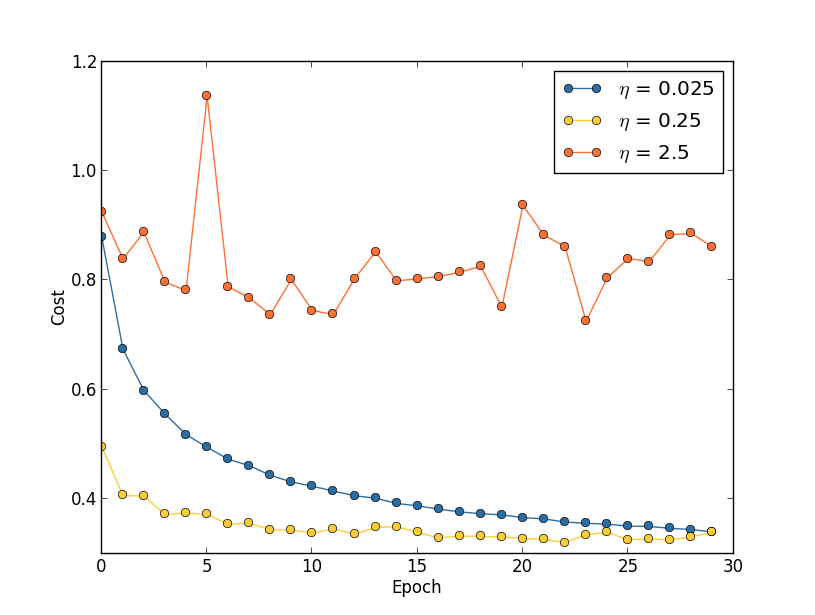
\includegraphics[width=0.867\textwidth]{images/multiple_eta.png}
\end{center}

\noindent 当 $\eta = 0.025$ 时，代价平滑下降直到最后一个轮次. 当 $\eta = 0.25$ 时，代价最初下降，但在大约 $20$ 个轮次后接近饱和，此后大部分变化只是微小且看似随机的振荡. 最后，当 $\eta = 2.5$ 时，代价从一开始就产生大幅振荡. 要理解振荡的原因，回想一下随机梯度下降应该引导我们逐渐下降到代价函数的一个谷底，

\begin{center}
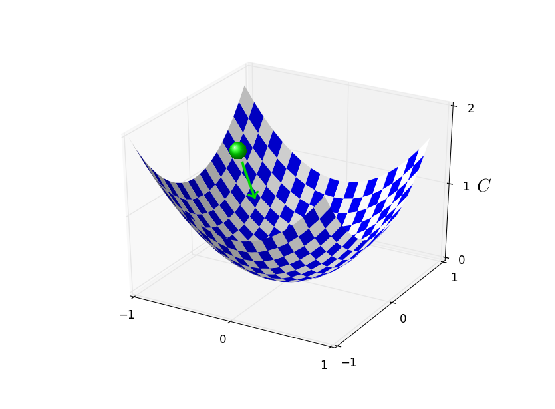
\includegraphics[width=0.9\textwidth]{images/tikz33.png}
\end{center}
\noindent 然而，如果 $\eta$ 太大，那么步长会大到实际上可能越过最小值，反而导致算法从谷底爬出来. 这很可能*\footnote{这个图景很有帮助，但它旨在作为可能发生情况的直觉性说明，而不是完整详尽的解释. 简而言之，更完整的解释如下：梯度下降使用代价函数的一阶近似来指导如何降低代价. 对于较大的 $\eta$，代价函数中的高阶项变得更加重要，并可能主导行为，导致梯度下降失效. 当我们接近代价函数的极小值和准极小值时，这种情况尤其可能发生，因为在这些点附近梯度变得很小，使得高阶项更容易主导行为.}就是当 $\eta = 2.5$ 时代价发生振荡的原因. 当我们选择 $\eta = 0.25$ 时，初始步骤确实将我们带向代价函数的极小值，只有当我们接近该极小值时，才开始受到过冲问题的影响. 而当我们选择 $\eta = 0.025$ 时，在前 $30$ 轮次中我们完全不会受到这个问题的影响. 当然，选择如此小的 $\eta$ 会带来另一个问题，即它会减慢随机梯度下降. 一个更好的方法是从 $\eta = 0.25$ 开始，训练 $20$ 轮次，然后切换到 $\eta = 0.025$. 我们稍后会讨论这种可变学习率日程\label{term:58}. 不过现在，让我们先专注于如何为学习率 $\eta$ 找到一个好的单一取值.

有了这个图景，我们可以按如下方式设定 $\eta$. 首先，我们估计 $\eta$ 的阈值，即训练数据上的代价立即开始下降而非振荡或上升的那个值. 这个估计不需要太精确. 你可以从 $\eta = 0.01$ 开始来估计数量级. 如果代价在前几轮次中下降，那么你应该依次尝试 $\eta = 0.1, 1.0, \ldots$，直到你找到一个 $\eta$ 值，使得代价在前几轮次中振荡或上升. 反之，如果在 $\eta = 0.01$ 时代价在前几轮次中振荡或上升，那么尝试 $\eta = 0.001, 0.0001, \ldots$，直到你找到一个 $\eta$ 值，使得代价在前几轮次中下降. 按照这个过程，我们将得到 $\eta$ 阈值的一个数量级估计. 你可以选择性地细化你的估计，找出代价在前几轮次中下降的最大 $\eta$ 值，比如 $\eta = 0.5$ 或 $\eta = 0.2$（这不需要非常精确）. 这样我们就得到了 $\eta$ 阈值的一个估计.

显然，你实际使用的 $\eta$ 值不应大于阈值. 事实上，如果 $\eta$ 的值要在许多轮次中保持可用，那么你可能希望使用一个更小的 $\eta$ 值，比如比阈值低两倍. 这样的选择通常能让你训练许多轮次，而不会导致学习速度过于缓慢.

在 MNIST 数据的情况下，遵循这一策略可以得到 $\eta$ 阈值的数量级估计为 $0.1$. 经过进一步细化，我们得到阈值 $\eta = 0.5$. 按照上述处方，这建议使用 $\eta = 0.25$ 作为我们的学习率取值. 事实上，我发现使用 $\eta = 0.5$ 在 $30$ 轮次中效果足够好，以至于大多数情况下我都不担心使用更低的 $\eta$ 值.

这一切看起来相当直接. 然而，使用训练代价来选择 $\eta$ 似乎与我在本节前面所说的相矛盾，即我们会通过使用留出的验证数据评估性能来选择超参数. 事实上，我们将使用验证准确率来选择正则化超参数、小批量大小以及网络参数（如层数和隐藏神经元数量等）. 为什么对学习率要区别对待呢？坦率地说，这个选择是我个人的审美偏好，也许有些特立独行. 理由是其他超参数旨在提高测试集上的最终分类准确率，因此基于验证准确率来选择它们是合理的. 然而，学习率只是附带地影响最终分类准确率. 它的主要目的实际上是控制梯度下降中的步长，而监控训练代价是检测步长是否过大的最佳方式. 话虽如此，这确实是一种个人审美偏好. 在学习早期，训练代价通常只在验证准确率提高时才会下降，因此实践中使用哪种标准不太可能产生太大差异.\textbf{使用提前停止来确定训练轮次数量：}正如我们在本章前面所讨论的，提前停止意味着在每个轮次结束时，我们应该计算验证数据上的分类准确率. 当它不再提高时，就终止. 这使得设置轮次数量变得非常简单. 特别是，这意味着我们不需要担心显式地弄清楚轮次数量如何依赖于其他超参数. 相反，这是自动处理的. 此外，提前停止还能自动防止我们过拟合. 这当然是一件好事，不过在实验的早期阶段，关闭提前停止可能是有帮助的，这样你可以看到任何过拟合的迹象，并利用它来指导你的正则化方法.

要实现提前停止，我们需要更精确地说明分类准确率停止提高意味着什么. 正如我们所看到的，准确率可能会大幅波动，即使整体趋势是提高的. 如果我们在准确率第一次下降时就停止，那么我们几乎肯定会在还有更多改进空间时就停止. 一个更好的规则是，如果最佳分类准确率在相当长一段时间内没有提高，就终止. 例如，假设我们正在做 MNIST. 那么我们可以选择在分类准确率在过去十轮次中没有提高时终止. 这确保了我们不会因为训练中的坏运气而停止得太早，同时也确保我们不会永远等待一个永远不会到来的改进.

这个“十轮次无改进”规则对于 MNIST 的初步探索是好的. 然而，网络有时会在某个特定分类准确率附近停滞相当长一段时间，然后又开始提高. 如果你试图获得真正好的性能，“十轮次无改进”规则可能在停止方面过于激进. 在这种情况下，我建议在初步实验中使用“十轮次无改进”规则，随着你更好地理解网络的训练方式，逐渐采用更宽松的规则：“二十轮次无改进”、“五十轮次无改进”等等. 当然，这引入了一个新的需要优化的超参数！然而在实践中，通常很容易设置这个超参数来获得相当好的结果. 同样，对于 MNIST 以外的问题，“十轮次无改进”规则可能过于激进或远远不够激进，这取决于问题的细节. 然而，通过一点实验，通常很容易找到一个相当好的提前停止策略.

到目前为止，我们在 MNIST 实验中还没有使用提前停止. 原因是我们一直在进行大量不同学习方法的比较. 对于这样的比较，在每个情况下使用相同的轮次数量是有帮助的. 然而，修改 \texttt{network2.py} 来实现提前停止是非常值得的：

\begin{exerciseBox}{习题}

\begin{itemize}

\item 修改 \texttt{network2.py}，使其使用“$n$ 轮次无改进”策略实现提前停止，其中 $n$ 是一个可以设置的参数.

\item 你能想到一个\emph{不同于}“$n$ 轮次无改进”的提前停止规则吗？理想情况下，该规则应该在获得高验证准确率和不过度训练之间取得折中. 将你的规则添加到 \texttt{network2.py} 中，并运行三个实验，将验证准确率和训练轮次数量与“$10$ 轮次无改进”进行比较.

\end{itemize}

\textbf{学习率日程：}我们一直保持学习率 $\eta$ 不变. 然而，变化学习率通常是有利的. 在学习过程的早期，权重很可能是严重错误的. 因此，最好使用较大的学习率，使权重快速变化. 之后，当我们对权重进行更精细的调整时，可以降低学习率.

我们应该如何设置学习率日程？有许多可能的方法. 一种自然的方法是使用与提前停止相同的基本思想. 其思想是保持学习率不变，直到验证准确率开始变差. 然后将学习率降低某个量，比如两倍或十倍. 我们重复这个过程多次，直到学习率比初始值低 $1,024$（或 $1,000$）倍. 然后我们终止.

可变学习日程可以提高性能，但它也打开了学习日程可能选择的世界. 这些选择可能令人头疼——你可以永远花时间试图优化你的学习日程. 对于初步实验，我的建议是使用单一的恒定学习率值. 这会给你一个很好的初步近似. 之后，如果你想从网络中获得最佳性能，值得按照我所描述的思路尝试学习日程*\footnote{一篇可读的近期论文展示了可变学习率在攻克 MNIST 时的优势，即 Deep, Big, Simple Neural Nets Excel on Handwritten Digit Recognition，作者为 Dan Claudiu Cireșan、Ueli Meier、Luca Maria Gambardella 和 Jürgen Schmidhuber（2010）.}.

\end{exerciseBox}

\begin{exerciseBox}{练习}

\begin{itemize}

\item 修改 \texttt{network2.py}，使其实现一个学习日程：每当验证准确率满足“$10$ 轮次无改进”规则时将学习率减半；并在学习率降至其原始值的 $1/128$ 时终止.

\end{itemize}

\textbf{正则化参数 $\lambda$：}我建议最初从无正则化（$\lambda = 0.0$）开始，并如上所述确定 $\eta$ 的值. 使用该 $\eta$ 选择，我们可以然后使用验证数据来选择 $\lambda$ 的一个好的值. 从试验 $\lambda = 1.0$*\footnote{我没有好的有原则的理由来使用这个作为起始值. 如果有人知道关于 $\lambda$ 从哪里开始的有原则的讨论，我将很感激听到它（mn@michaelnielsen.org）.}开始，然后根据需要以 $10$ 的倍数增加或减少，以提高验证数据上的性能. 一旦你找到了一个好的数量级，你就可以微调你的 $\lambda$ 值. 完成后，你应该返回并再次重新优化 $\eta$.

\end{exerciseBox}

\begin{exerciseBox}{练习}

\begin{itemize}

\item 使用梯度下降来尝试学习 $\lambda$ 和 $\eta$ 等超参数的好值是很有诱惑力的. 你能想到使用梯度下降来确定 $\lambda$ 的一个障碍吗？你能想到使用梯度下降来确定 $\eta$ 的一个障碍吗？

\end{itemize}

\textbf{我在本书前面是如何选择超参数的：}如果你使用本节的建议，你会发现你得到的 $\eta$ 和 $\lambda$ 值并不总是与我在本书前面使用的值完全匹配. 原因是本书有叙事上的限制，有时使得优化超参数变得不切实际. 想想我们做过的所有不同学习方法的比较，例如，比较二次代价函数和交叉熵代价函数，比较新旧权重初始化方法，在有和没有正则化的情况下运行，等等. 为了使这样的比较有意义，我通常试图在比较的方法之间保持超参数不变（或以适当的方式缩放它们）. 当然，没有理由相同的超参数对所有不同的学习方法都是最优的，所以我使用的超参数是一种折中.

作为这种折中的替代方案，我本可以尝试为每一种学习方法最大限度地优化超参数. 原则上，那将是一种更好、更公平的方法，因为那样我们就能看到每种学习方法的最佳表现. 然而，我们沿着这些思路做了几十次比较，实践中我发现计算成本太高. 这就是为什么我采用了使用相当好（但不一定最优）的超参数选择的折中方案.\textbf{小批量大小：}我们应该如何设置小批量大小？为了回答这个问题，让我们首先假设我们正在做在线学习，即我们使用的小批量大小为 $1$.

关于在线学习的明显担忧是，使用仅包含单个训练样本的小批量会导致我们的梯度估计出现显著误差. 然而事实上，这些误差结果证明并不是什么大问题. 原因是个体梯度估计不需要非常精确. 我们所需要的只是一个足够精确的估计，使我们的代价函数倾向于持续下降. 这就好像你试图到达北磁极，但有一个不稳定的指南针，每次你看它时都偏离 10-20 度. 只要你经常停下来检查指南针，并且指南针平均而言方向正确，你最终就能顺利到达北磁极.

基于这个论证，听起来我们应该使用在线学习. 事实上，情况结果证明比这更复杂. 在上一章的一个习题中，我指出可以使用矩阵技术同时计算小批量中\emph{所有}样本的梯度更新，而不是对它们进行循环. 取决于你的硬件和线性代数库的细节，这可以使计算（例如）大小为 $100$ 的小批量的梯度估计比通过分别循环 $100$ 个训练样本来计算小批量梯度估计快相当多. 它可能只需要（比如说）$50$ 倍的时间，而不是 $100$ 倍的时间.

现在，起初这似乎对我们帮助不大. 对于大小为 $100$ 的小批量，权重的学习规则看起来像：

\begin{equation}
w \rightarrow w' = w-\eta \frac{1}{100} \sum_x \nabla C_x,
\tag{100}
\end{equation}

\noindent 其中求和是对小批量中的训练样本进行的. 这对比于

\begin{equation}
w \rightarrow w' = w-\eta \nabla C_x
\tag{101}
\end{equation}

\noindent 在线学习的情况. 即使做小批量更新只需要 $50$ 倍的时间，看起来仍然可能更好地做在线学习，因为我们会更新得频繁得多. 然而，假设在小批量情况下我们将学习率增加 $100$ 倍，那么更新规则变为

\begin{equation}
w \rightarrow w' = w-\eta \sum_x \nabla C_x.
\tag{102}
\end{equation}

\noindent 这很像以学习率 $\eta$ 做 $100$ 次独立的在线学习. 但它只需要做单次在线学习 $50$ 倍的时间. 当然，它与 $100$ 次在线学习并不完全相同，因为在小批量中所有 $\nabla C_x$ 都是在同一组权重下评估的，而不是在线学习情况下发生的累积学习. 尽管如此，使用更大的小批量似乎明显有可能加快速度.

考虑到这些因素，选择最佳小批量大小是一种折中. 太小，你就无法充分利用为快速硬件优化的优秀矩阵库的优势. 太大，你就只是没有足够频繁地更新权重. 你需要的是选择一个折中值，使学习速度最大化. 幸运的是，速度最大化时的小批量大小选择相对独立于其他超参数（除了整体架构），所以你不需要先优化那些超参数就能找到好的小批量大小. 因此，方法是使用一些可接受的（但不一定最优的）其他超参数值，然后试验若干不同的小批量大小，如上所述缩放 $\eta$. 绘制验证准确率与\emph{时间}（即实际经过的时间，而不是轮次！）的关系，并选择能给你带来最快性能提升的小批量大小. 选定了小批量大小后，你就可以继续优化其他超参数了.

当然，正如你无疑已经意识到的，我在我们的工作中没有做这种优化. 事实上，我们的实现根本没有使用更快的小批量更新方法. 在几乎所有例子中，我只是简单地使用了小批量大小 $10$，没有评论或解释. 因此，我们本可以通过减小小批量大小来加速学习. 我没有这样做，部分是因为我想说明使用大于 $1$ 的小批量，部分是因为我的初步实验表明加速会相当有限. 然而，在实际实现中，我们肯定会实现更快的小批量更新方法，然后努力优化小批量大小，以最大化我们的整体速度.\textbf{自动化技术：}我一直在描述这些启发式方法，就好像你在手动优化超参数. 手动优化是建立对神经网络行为直觉的好方法. 然而，不出所料，在自动化这个过程方面已经做了大量工作. 一种常见的技术是\emph{网格搜索}，它在超参数空间中系统地搜索一个网格. 关于网格搜索的成就和局限性的综述（附有易于实现的替代方案的建议）可以在 James Bergstra 和 Yoshua Bengio 的 2012 年论文*\footnote{Random search for hyper-parameter optimization，作者为 James Bergstra 和 Yoshua Bengio（2012）.}中找到. 许多更复杂的方法也被提出了. 我不会在这里综述所有这些工作，但想提到一篇特别有前景的 2012 年论文，它使用贝叶斯方法来自动优化超参数*\footnote{Practical Bayesian optimization of machine learning algorithms，作者为 Jasper Snoek、Hugo Larochelle 和 Ryan Adams.}. 该论文的代码是公开可用的，并已被其他研究人员取得了一些成功.\textbf{总结：}遵循我所描述的经验法则不会从你的神经网络中获得绝对最好的可能结果. 但它很可能会给你一个好的开始和进一步改进的基础. 特别是，我基本上是独立地讨论超参数的. 实践中，超参数之间存在关系. 你可能会试验 $\eta$，觉得你已经把它调得恰到好处，然后开始优化 $\lambda$，却发现它打乱了你对 $\eta$ 的优化. 实践中，来回反复调整，逐渐逼近好的值是有帮助的. 最重要的是，记住我所描述的启发式方法是经验法则，不是一成不变的规则. 你应该留意事情不奏效的迹象，并愿意进行实验. 特别是，这意味着仔细监控你的网络行为，尤其是验证准确率.

选择超参数的困难因以下事实而加剧：关于如何选择超参数的知识广泛分散在许多研究论文和软件程序中，而且往往只存在于个别实践者的头脑中. 有许许多多的论文提出了（有时相互矛盾的）关于如何进行的建议. 然而，有几篇特别有用的论文综合并提炼了这些知识中的大部分.Yoshua Bengio 有一篇 2012 年的论文*\footnote{Practical recommendations for gradient-based training of deep architectures，作者为 Yoshua Bengio（2012）.}，给出了一些使用反向传播和梯度下降来训练神经网络（包括深度神经网络）的实用建议.Bengio 比我更详细地讨论了许多问题，包括如何进行更系统的超参数搜索. 另一篇好论文是 Yann LeCun、Léon Bottou、Genevieve Orr 和 Klaus-Robert Müller 的 1998 年论文*\footnote{Efficient BackProp，作者为 Yann LeCun、Léon Bottou、Genevieve Orr 和 Klaus-Robert Müller（1998）.}. 这两篇论文都出现在一本极其有用的 2012 年书籍中，该书收集了神经网络中常用的许多技巧*\footnote{Neural Networks: Tricks of the Trade，由 Grégoire Montavon、Geneviève Orr 和 Klaus-Robert Müller 编辑.}. 这本书很贵，但许多文章已被各自作者放到网上，想必得到了出版商的许可，可以使用搜索引擎找到.

当你阅读这些文章时，尤其是当你进行自己的实验时，有一件事变得很清楚：超参数优化从来不是一个完全解决的问题. 总还有另一个技巧可以尝试来提高性能. 作家中有一句常说的话：书永远不会完成，只会被放弃. 神经网络优化也是如此：超参数空间如此之大，以至于人永远不会真正完成优化，只会将网络遗留给后世. 所以你的目标应该是开发一种工作流程，使你能够快速地在优化上做得相当好，同时保留灵活性，以便在重要时尝试更详细的优化.

设置超参数的挑战使一些人抱怨神经网络与其他机器学习技术相比需要大量工作. 我听过以下抱怨的许多变体：``是的，一个调好的神经网络可能在该问题上获得最佳性能. 但另一方面，我可以尝试随机森林 [或 SVM 或$\ldots$ 插入你自己喜欢的技术]，它就能直接工作. 我没有时间弄清楚恰好正确的神经网络.''当然，从实际角度来看，拥有易于应用的技术是好的. 当你刚刚开始一个问题，而且机器学习是否能帮助解决这个问题可能还不明显时，这一点尤其正确. 另一方面，如果获得最优性能很重要，那么你可能需要尝试需要更多专业知识的方案. 虽然机器学习总是很简单就好了，但没有\emph{先验}理由表明它应该是轻而易举的.

\end{exerciseBox}
\sectionTitle{其他技术}{其他技术}

本章中发展的每一项技术本身都值得了解，但这并不是我解释它们的唯一原因. 更重要的目的是让你熟悉神经网络中可能出现的一些问题，以及一种有助于克服这些问题的分析风格. 从某种意义上说，我们一直在学习如何思考神经网络. 在本章的剩余部分，我将简要概述另外几项技术. 这些概述不如之前的讨论那样深入，但应当能让你感受到可用于神经网络的技术之多样.
\subsectionTitle{随机梯度下降的变体}{随机梯度下降的变体}

通过反向传播实现的随机梯度下降在解决 MNIST 数字分类问题上一直表现良好. 然而，还有许多其他优化代价函数的方法，有时这些其他方法能提供优于小批量随机梯度下降的性能. 在本节中，我概述两种这样的方法： Hessian 方法和动量方法. \textbf{Hessian 方法：} 为了开始我们的讨论，暂且把神经网络放在一边会有所帮助. 相反，我们只考虑最小化代价函数 $C$ 的抽象问题， $C$ 是许多变量的函数， $w = w_1, w_2, \ldots$，所以 $C = C(w)$. 根据泰勒定理，代价函数可以在点 $w$ 附近近似为

\begin{align}
C(w+\Delta w) &= C(w) + \sum_j \frac{\partial C}{\partial w_j} \Delta w_j \nonumber \\ & & + \frac{1}{2} \sum_{jk} \Delta w_j \frac{\partial^2 C}{\partial w_j \partial w_k} \Delta w_k + \ldots \tag{103}
\end{align}

\noindent 我们可以更紧凑地将其重写为

\begin{equation}
C(w+\Delta w) = C(w) + \nabla C \cdot \Delta w + \frac{1}{2} \Delta w^T H \Delta w + \ldots,
\tag{104}
\end{equation}

\noindent 其中 $\nabla C$ 是通常的梯度向量， $H$ 是一个称为 \emph{Hessian 矩阵}的矩阵，其 $jk$ 项为 $\partial^2 C / \partial w_j \partial w_k$. 假设我们通过丢弃上面由 $\ldots$ 表示的高阶项来近似 $C$,

\begin{equation}
C(w+\Delta w) \approx C(w) + \nabla C \cdot \Delta w + \frac{1}{2} \Delta w^T H \Delta w.
\tag{105}
\end{equation}

\noindent 使用微积分我们可以证明，通过选择以下式子，右侧的表达式可以被最小化*\footnote{严格来说，要使其成为最小值而不仅仅是极值，我们需要假设 Hessian 矩阵是正定的. 直观地说，这意味着函数 $C$ 局部看起来像一个山谷，而不是山峰或鞍点.}

\begin{equation}
\Delta w = -H^{-1} \nabla C.
\tag{106}
\end{equation}

\noindent 只要 (105)

\begin{align*}
C(w+\Delta w) \approx C(w) + \nabla C \cdot \Delta w + \frac{1}{2} \Delta w^T H \Delta w \nonumber
\end{align*}

\noindent 是代价函数的一个良好近似表达式，那么我们可以预期从点 $w$ 移动到 $w+\Delta w = w-H^{-1} \nabla C$ 应该会显著减小代价函数. 这提示了一个可能的最小化代价的算法：

\begin{itemize}

\item 选择一个起始点 $w$.

\item 将 $w$ 更新为新点 $w' = w-H^{-1} \nabla C$，其中 Hessian $H$ 和 $\nabla C$ 在 $w$ 处计算.

\item 将 $w'$ 更新为新点 $w{'}{'} = w'-H'^{-1} \nabla' C$，其中 Hessian $H'$ 和 $\nabla' C$ 在 $w'$ 处计算.

\item $\ldots$

\end{itemize}

在实践中， (105)

\begin{align*}
C(w+\Delta w) \approx C(w) + \nabla C \cdot \Delta w + \frac{1}{2} \Delta w^T H \Delta w \nonumber
\end{align*}

\noindent 只是一个近似，采取较小的步长会更好. 我们通过反复将 $w$ 改变 $\Delta w = -\eta H^{-1} \nabla C$ 来实现这一点，其中 $\eta$ 被称为学习率.

这种最小化代价函数的方法被称为 \emph{Hessian 方法}或 \emph{Hessian 优化}. 有理论和实证结果表明， Hessian 方法比标准梯度下降以更少的步数收敛到最小值. 特别是，通过纳入关于代价函数二阶变化的信息， Hessian 方法有可能避免梯度下降中可能出现的许多病态情况. 此外，还有可以用于计算 Hessian 的反向传播算法版本.

如果 Hessian 优化如此出色，为什么我们不在神经网络中使用它呢？不幸的是，尽管它有许多理想的特性，但它有一个非常不受欢迎的特性：它在实践中非常难以应用. 部分问题在于 Hessian 矩阵的规模巨大. 假设你有一个具有 $10^7$ 个权重和偏置的神经网络. 那么相应的 Hessian 矩阵将包含 $10^7 \times 10^7 = 10^{14}$ 个元素. 那可是很多元素！这使得在实践中计算 $H^{-1} \nabla C$ 极其困难. 然而，这并不意味着理解它没有用. 事实上，有许多梯度下降的变体受到 Hessian 优化的启发，但避免了矩阵过大的问题. 让我们来看一种这样的技术：基于动量的梯度下降. \textbf{基于动量的梯度下降：} 直观地说， Hessian 优化的优势在于它不仅纳入了关于梯度的信息，还纳入了关于梯度如何变化的信息. 基于动量的梯度下降基于类似的直觉，但避免了大型的二阶导数矩阵. 要理解动量技术，回想一下我们最初关于梯度下降的图景，其中我们考虑了一个滚入山谷的球. 当时，我们观察到梯度下降尽管名字如此，但只是粗略地类似于球落入谷底. 动量技术以两种方式修改梯度下降，使其更接近物理图景. 首先，它为我们试图优化的参数引入了``速度''的概念. 梯度作用于改变速度，而不是(直接)改变``位置''，这与物理力改变速度，仅间接影响位置非常相似. 其次，动量方法引入了一种摩擦力项，它倾向于逐渐减小速度.

让我们给出更精确的数学描述. 我们引入速度变量 $v = v_1, v_2, \ldots$，每个对应于相应的 $w_j$ 变量*\footnote{在神经网络中， $w_j$ 变量当然会包括所有权重和偏置.}. 然后我们将梯度下降更新规则 $w \rightarrow w'= w-\eta \nabla C$ 替换为

\begin{align}
v &\rightarrow v' = \mu v - \eta \nabla C \tag{107} \\ w &\rightarrow w' = w+v'. \tag{108}
\end{align}

\noindent 在这些方程中， $\mu$ 是一个超参数，控制系统中的阻尼或摩擦量. 要理解这些方程的含义，首先考虑 $\mu = 1$ 的情况会有所帮助，这对应于没有摩擦. 在这种情况下，检查方程表明``力'' $\nabla C$ 现在正在修改速度 $v$，而速度控制着 $w$ 的变化率. 直观地说，我们通过反复向速度添加梯度项来积累速度. 这意味着如果梯度在几轮学习中(大致)沿同一方向，我们就可以在该方向上积累相当多的动量. 例如，想想如果我们正沿着斜坡直线下降会发生什么：

\begin{center}
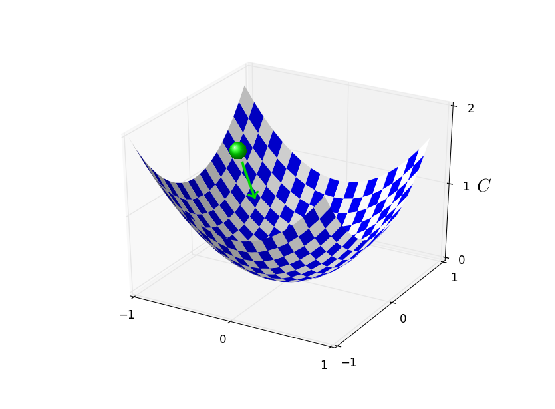
\includegraphics[width=0.9\textwidth]{images/tikz34.png}
\end{center}

\noindent 每走一步，沿斜坡向下的速度就会增大，因此我们越来越快地移动到谷底. 这可以使动量技术比标准梯度下降快得多. 当然，一个问题是，一旦我们到达谷底，我们就会冲过头. 或者，如果梯度变化很快，那么我们可能会发现自己朝着错误的方向移动. 这就是 (107) 中 $\mu$ 超参数的原因

\begin{align*}
v &\rightarrow v' = \mu v - \eta \nabla C \nonumber
\end{align*}

\noindent. 我之前说过 $\mu$ 控制系统中的摩擦量；更精确地说，你应该将 $1-\mu$ 视为系统中的摩擦量. 当 $\mu = 1$ 时，正如我们所看到的，没有摩擦，速度完全由梯度 $\nabla C$ 驱动. 相反，当 $\mu = 0$ 时，有很大的摩擦，速度无法积累，方程 (107)

\begin{align*}
v &\rightarrow v' = \mu v - \eta \nabla C \nonumber
\end{align*}

\noindent 和 (108)

\begin{align*}
w &\rightarrow w' = w+v' \nonumber
\end{align*}

\noindent 简化为通常的梯度下降方程 $w \rightarrow w'=w-\eta \nabla C$. 在实践中，使用介于 $0$ 和 $1$ 之间的 $\mu$ 值可以给我们带来能够积累速度的大部分好处，而不会导致冲过头. 我们可以使用留出的验证数据来选择这样的 $\mu$ 值，就像我们选择 $\eta$ 和 $\lambda$ 一样.

到目前为止，我一直避免给超参数 $\mu$ 命名. 原因是 $\mu$ 的标准名称选择得很糟糕：它被称为 \emph{动量系数}. 这可能会引起混淆，因为 $\mu$ 与物理学中的动量概念完全不同. 相反，它与摩擦的关系更为密切. 然而，动量系数这个术语被广泛使用，所以我们将继续使用它.

动量技术的一个好处是，修改梯度下降的实现以纳入动量几乎不需要任何工作. 我们仍然可以使用反向传播来计算梯度，就像以前一样，并使用诸如随机选择小批量样本之类的想法. 通过这种方式，我们可以获得 Hessian 方法的一些优势，利用关于梯度如何变化的信息. 但这样做没有缺点，并且只需要对我们的代码进行微小的修改. 在实践中，动量技术被普遍使用，并且经常加速学习.

\begin{exerciseBox}{练习}

\begin{itemize}

\item 如果我们在动量技术中使用 $\mu > 1$ 会出什么问题？

\item 如果我们在动量技术中使用 $\mu < 0$ 会出什么问题？

\end{itemize}

\end{exerciseBox}

\begin{exerciseBox}{习题}

\begin{itemize}

\item 将基于动量的随机梯度下降添加到 \texttt{network2.py} 中.

\end{itemize}

\textbf{其他最小化代价函数的方法：} 许多其他最小化代价函数的方法已经被开发出来，对于哪种方法最好并没有普遍的共识. 当你更深入地研究神经网络时，值得深入研究其他技术，理解它们的工作原理，优缺点，以及如何在实际中应用它们. 我之前提到的一篇论文*\footnote{Efficient BackProp, by Yann LeCun, Léon Bottou, Genevieve Orr and Klaus-Robert Müller (1998).} 介绍并比较了其中几种技术，包括共轭梯度下降和 BFGS 方法(另见密切相关的有限内存 BFGS 方法，称为 L-BFGS). 另一种最近显示出有希望结果的技术*\footnote{See, for example, On the importance of initialization and momentum in deep learning, by Ilya Sutskever, James Martens, George Dahl, and Geoffrey Hinton (2012).} 是 Nesterov 加速梯度技术，它改进了动量技术. 然而，对于许多问题，普通的随机梯度下降效果很好，特别是如果使用动量，因此在本书的剩余部分我们将坚持使用随机梯度下降.

\end{exerciseBox}
\subsectionTitle{人工神经元的其他模型}{人工神经元的其他模型}

到目前为止，我们一直使用 S 型神经元来构建神经网络. 原则上，由 S 型神经元构成的网络可以计算任意函数. 然而在实践中，使用其他模型神经元构建的网络有时会优于 S 型网络. 根据应用的不同，基于这些替代模型的网络可能学习得更快、对测试数据泛化得更好，或者两者兼而有之. 让我介绍几种替代模型神经元，让你感受一下一些常用变体的风格.

也许最简单的变体是 tanh（读作 ``tanch''）神经元，它用双曲正切函数取代了 S 型函数. 一个 tanh 神经元在输入 $x$、权重向量 $w$ 和偏置 $b$ 下的输出由下式给出

\begin{equation}
\tanh(w \cdot x+b),
\tag{109}
\end{equation}

\noindent 其中 $\tanh$ 当然就是双曲正切函数. 事实证明，它与 S 型神经元密切相关. 要看出这一点，回想一下 $\tanh$ 函数的定义是

\begin{equation}
\tanh(z) \equiv \frac{e^z-e^{-z}}{e^z+e^{-z}}.
\tag{110}
\end{equation}

\noindent 稍作代数运算便可轻易验证

\begin{equation}
\sigma(z) = \frac{1+\tanh(z/2)}{2},
\tag{111}
\end{equation}

\noindent 也就是说，$\tanh$ 只不过是 S 型函数的一个重新缩放版本. 我们也可以从图形上看出 $\tanh$ 函数与 S 型函数具有相同的形状.tanh 神经元与 S 型神经元的一个区别在于，tanh 神经元的输出范围是 -1 到 1，而不是 0 到 1. 这意味着如果你要构建一个基于 tanh 神经元的网络，你可能需要以与 S 型网络略有不同的方式对你的输出（并且，根据应用的具体细节，可能还有你的输入）进行规范化\label{term:59}.

与 S 型神经元类似，tanh 神经元构成的网络原则上可以计算任意函数*\footnote{对于 tanh 神经元和 S 型神经元，以及下面讨论的修正线性神经元，这一说法都有一些技术上的注意事项. 不过，非正式地说，通常可以把神经网络理解为能够以任意精度近似任意函数.}，将输入映射到 -1 到 1 的范围. 此外，诸如反向传播和随机梯度下降之类的思想，应用于 tanh 神经元网络与应用于 S 型神经元网络一样容易.

\begin{exerciseBox}{练习}

\begin{itemize}

\item
证明方程 (111) 中的恒等式

\begin{align*}
\sigma(z) = \frac{1+\tanh(z/2)}{2} \nonumber
\end{align*}

.

\end{itemize}

你应该在网络中使用哪种类型的神经元，tanh 还是 S 型？\emph{先验地} 说，答案并不明显，说得委婉一点！然而，有理论论证和一些经验证据表明 tanh 有时表现更好*\footnote{例如，参见 Yann LeCun、Léon Bottou、Genevieve Orr 和 Klaus-Robert Müller (1998) 的 Efficient BackProp，以及 Xavier Glorot 和 Yoshua Bengio (2010) 的 Understanding the difficulty of training deep feedforward networks.}. 让我简要地介绍一下支持 tanh 神经元的其中一个理论论证的风格. 假设我们使用 S 型神经元，因此网络中所有的激活值都是正的. 让我们考虑输入到第 $l+1$ 层第 $j$ 个神经元的权重 $w^{l+1}_{jk}$. 反向传播的规则（见此处）告诉我们，相关的梯度将是 $a^l_k \delta^{l+1}_j$. 因为激活值是正的，这个梯度的符号将与 $\delta^{l+1}_j$ 的符号相同. 这意味着如果 $\delta^{l+1}_j$ 是正的，那么在梯度下降过程中 \emph{所有} 权重 $w^{l+1}_{jk}$ 都会减小，而如果 $\delta^{l+1}_j$ 是负的，那么在梯度下降过程中 \emph{所有} 权重 $w^{l+1}_{jk}$ 都会增大. 换句话说，连接到同一个神经元的所有权重必须要么一起增大，要么一起减小. 这是个问题，因为有些权重可能需要增大而另一些需要减小. 只有当某些输入激活值具有不同的符号时，这种情况才可能发生. 这提示我们用一种允许正负激活值的激活函数来取代 S 型函数，例如 $\tanh$. 事实上，因为 $\tanh$ 关于零对称，$\tanh(-z) = -\tanh(z)$，我们甚至可以期望，粗略地说，隐藏层中的激活值会在正负之间大致均衡. 这将有助于确保权重更新不会系统性地偏向某一个方向.

我们应该多认真地对待这个论证呢？虽然这个论证很有启发性，但它只是一种启发式推理，而不是 tanh 神经元优于 S 型神经元的严格证明. 也许 S 型神经元还有其他特性可以弥补这个问题？事实上，对于许多任务，经验上发现 tanh 相比 S 型神经元只能带来很小的性能提升，甚至没有提升. 不幸的是，对于任何特定的应用，我们还没有确定不移的规则来知道哪种神经元类型学习最快，或者给出最好的泛化性能.

S 型神经元的另一种变体是 \emph{修正线性神经元} 或 \emph{修正线性单元}. 一个修正线性单元在输入 $x$、权重向量 $w$ 和偏置 $b$ 下的输出由下式给出

\begin{equation}
\max(0, w \cdot x+b).
\tag{112}
\end{equation}

\noindent 从图形上看，修正函数 $\max(0, z)$ 看起来是这样的：显然，这类神经元与 S 型神经元和 tanh 神经元都相当不同. 然而，与 S 型神经元和 tanh 神经元一样，修正线性单元\label{term:60}可以用来计算任意函数，并且可以使用反向传播和随机梯度下降之类的思想来训练.

什么时候你应该使用修正线性单元而不是 S 型或 tanh 神经元？一些最近的图像识别工作*\footnote{例如，参见 Kevin Jarrett、Koray Kavukcuoglu、Marc'Aurelio Ranzato 和 Yann LeCun (2009) 的 What is the Best Multi-Stage Architecture for Object Recognition？，Xavier Glorot、Antoine Bordes 和 Yoshua Bengio (2011) 的 Deep Sparse Rectifier Neural Networks，以及 Alex Krizhevsky、Ilya Sutskever 和 Geoffrey Hinton (2012) 的 ImageNet Classification with Deep Convolutional Neural Networks. 请注意，这些论文补充了关于在使用修正线性单元的网络中如何设置输出层、代价函数和正则化的重要细节. 在这个简要的叙述中，我忽略了所有这些细节. 这些论文还更详细地讨论了使用修正线性单元的利弊. 另一篇信息丰富的论文是 Vinod Nair 和 Geoffrey Hinton (2010) 的 Rectified Linear Units Improve Restricted Boltzmann Machines，它展示了在一种稍有不同的神经网络方法中使用修正线性单元的好处.} 发现在网络的大部分中使用修正线性单元有相当大的好处. 然而，与 tanh 神经元一样，我们还没有真正深入地理解究竟何时修正线性单元更可取，以及为什么. 为了让你感受一下其中一些问题，回想一下 S 型神经元在饱和时会停止学习，即当它们的输出接近 $0$ 或 $1$ 时. 正如我们在本章中反复看到的，问题在于 $\sigma'$ 项会减小梯度，从而减慢学习速度.tanh 神经元在饱和时也会遇到类似的问题. 相比之下，增大修正线性单元的加权输入永远不会使它饱和，因此不存在相应的学习减速. 另一方面，当修正线性单元的加权输入为负时，梯度消失，因此该神经元完全停止学习. 这些只是众多问题中的两个，它们使得理解修正线性单元何时以及为何比 S 型或 tanh 神经元表现更好变得并非易事.

我在这里描绘了一幅充满不确定性的图景，强调我们还没有一个关于应该如何选择激活函数的坚实理论. 事实上，问题比我描述的还要困难，因为存在无穷多种可能的激活函数. 对于任何给定的问题，哪一种最好？哪一种会导致网络学习最快？哪一种会给出最高的测试准确率？令我惊讶的是，对这些问题真正深入和系统的研究竟然如此之少. 理想情况下，我们会有一个理论，详细地告诉我们如何选择（也许还可以动态修改）我们的激活函数. 另一方面，我们不应该让缺乏完整理论阻碍我们！我们手头已经有强大的工具，可以用这些工具取得很多进展. 在本书的剩余部分，我将继续使用 S 型神经元作为我们的首选神经元，因为它们功能强大，并且为关于神经网络的核心思想提供了具体的例证. 但请记住，这些同样的思想也可以应用于其他类型的神经元，而且这样做有时会有优势.

\end{exerciseBox}
\subsectionTitle{关于神经网络中的故事}{关于神经网络中的故事}

\begin{quote}
\emph{\textbf{问题：}你如何着手利用和研究那些几乎完全由经验而非数学支撑的机器学习技术？另外，在哪些情况下你注意到其中一些技术会失败？\textbf{回答：}你必须意识到我们的理论工具非常薄弱. 有时，我们对某项特定技术为何有效有着良好的数学直觉. 有时我们的直觉最终被证明是错误的 [...] 问题就变成了：我的方法在这个特定问题上表现如何，以及它在多大的问题集合上表现良好.- 与神经网络研究者 Yann LeCun 的问答}
\end{quote}

有一次，我参加了一个关于量子力学基础的会议，我注意到一个在我看来非常奇特的口头习惯：当演讲结束时，听众的提问常常以 ``我非常赞同你的观点，但是 [...]'' 开头. 量子基础并非我通常的领域，我之所以注意到这种提问方式，是因为在其他科学会议上，我很少或从未听到提问者表达对演讲者观点的赞同. 当时，我认为这种提问的普遍性表明量子基础领域几乎没有取得真正的进展，人们只是在原地打转. 后来，我意识到这个评价过于苛刻. 演讲者们正在与人类心智所面对过的一些最困难的问题作斗争. 当然进展缓慢！但即使他们并不总是有无可争辩的新进展可以报告，听取人们思考方式的最新动态仍然是有价值的.

你可能已经注意到本书中有一个类似于 ``我非常赞同 [...]'' 的口头习惯. 为了解释我们所看到的现象，我常常退回到说 ``启发式地讲，[...]''，或者 ``粗略地说，[...]''，然后接着用一个故事来解释某个现象或其他东西. 这些故事是合理的，但我所呈现的经验证据往往相当薄弱. 如果你翻阅研究文献，你会看到类似风格的故事出现在许多关于神经网络的研究论文中，往往只有薄弱的支持证据. 我们应该如何看待这样的故事？

在科学的许多领域——尤其是那些处理简单现象的领域——有可能为相当普遍的假设获得非常坚实、非常可靠的证据. 但在神经网络中，存在大量的参数和超参数，以及它们之间极其复杂的相互作用. 在如此极其复杂的系统中，要建立可靠的普遍陈述是极其困难的. 从完全普遍的意义上理解神经网络，是一个像量子基础一样考验人类心智极限的问题. 相反，我们常常只能满足于支持或反对某个普遍陈述的少数具体实例的证据. 结果，当新的证据出现时，那些陈述有时后来需要被修改或放弃.

看待这种情况的一种方式是，任何关于神经网络的启发式故事都带有一种隐含的挑战. 例如，考虑我之前引用的那个陈述，解释 dropout 为何有效*\footnote{摘自 Alex Krizhevsky、Ilya Sutskever 和 Geoffrey Hinton 的 ImageNet Classification with Deep Convolutional Neural Networks (2012).}：``这种技术减少了神经元之间复杂的共适应，因为一个神经元不能依赖于特定其他神经元的存在. 因此，它被迫学习更稳健的特征，这些特征在与许多不同的其他神经元随机子集结合时是有用的.'' 这是一个丰富、具有挑衅性的陈述，人们完全可以围绕剖析这个陈述来建立一个富有成果的研究项目，弄清楚其中哪些是真的，哪些是假的，哪些需要变化和完善. 事实上，现在已经有一个小型的研究产业，研究者们在调查 dropout（以及许多变体），试图理解它如何工作，以及它的局限是什么. 我们讨论过的许多启发式方法也是如此. 每个启发式方法不仅是一个（潜在的）解释，也是一个需要更详细地调查和理解的挑战.

当然，没有任何一个人有时间去深入调查所有这些启发式解释. 神经网络研究者群体要发展出一个真正强大的、基于证据的关于神经网络如何学习的理论，将需要几十年（或更长时间）. 这是否意味着你应该拒绝启发式解释，认为它们不严谨、证据不足？不！事实上，我们需要这样的启发式方法来启发和指导我们的思考. 这就像伟大的探索时代：早期的探险家有时是在某些重要方面错误的信念基础上进行探索（并做出新发现）的. 后来，随着我们填补了地理知识，那些错误被纠正了. 当你对某件事理解得很差时——就像探险家对地理的理解，以及我们今天对神经网络的理解——大胆探索比在思考的每一步都严格正确更为重要. 因此，你应该把这些故事视为关于如何思考神经网络的有用指南，同时保持对这些故事局限性的健康意识，并仔细追踪任何给定推理路线的证据究竟有多强. 换句话说，我们需要好的故事来帮助激励和启发我们，也需要严谨的深入研究来揭示事情的真相.
